\documentclass{pre-tfg}

\usepackage{listings}
\usepackage{formular}
\usepackage[pdftex]{graphicx}
\usepackage{subcaption}
\usepackage[rightcaption]{sidecap}
\usepackage{hyperref}
\usepackage{todonotes}
\usepackage{amsmath}
\usepackage{verbatim}
\usepackage{apalike}

\showhelp  % comenta o borra para eliminar ayudas

\title{Identificación automática de personajes en textos de ficción pertenecientes al género fanfiction}
\author{María González Gutiérrez}
\advisorFirst{José Ángel Olivas Varela}
\docdate{2021}{Febrero}
\intensification{Computación}


\DeclareGraphicsExtensions{.pdf,.png,.jpg}

\usepackage{color}
\definecolor{gray97}{gray}{.97}
\definecolor{gray75}{gray}{.75}
\definecolor{gray45}{gray}{.45}

\lstset{ frame=Ltb,
     framerule=0pt,
     aboveskip=0.5cm,
     framextopmargin=3pt,
     framexbottommargin=3pt,
     framexleftmargin=0.4cm,
     framesep=0pt,
     rulesep=.4pt,
     backgroundcolor=\color{gray97},
     rulesepcolor=\color{black},
     %
     stringstyle=\ttfamily,
     showstringspaces = false,
     basicstyle=\small\ttfamily,
     commentstyle=\color{gray45},
     keywordstyle=\bfseries,
     %
     numbers=left,
     numbersep=15pt,
     numberstyle=\tiny,
     numberfirstline = false,
     breaklines=true,
   }

% minimizar fragmentado de listados
\lstnewenvironment{listing}[1][]
   {\lstset{#1}\pagebreak[0]}{\pagebreak[0]}

\lstdefinestyle{consola}
   {basicstyle=\scriptsize\ttfamily,
    %backgroundcolor=\color{gray75},
    keywordstyle=\bf\color{orange},
    commentstyle=\color{blue}, 
    stringstyle=\color{magenta},   
    captionpos=b,
    language=Python,
   }

\lstdefinestyle{C}
   {language=C,
   }


\renewcommand*\lstlistingname{Listado}

%% PLACEHOLDERS %%
\newcommand{\refToLinkScraperCode}{\ref{an:scrapers}}
\newcommand{\refToFileScraperCode}{\ref{an:scrapers}}


%\newcommand{\refToAnexoDatosRFE}{[placeholder ref]}

\newcommand{\finalProgramName}{fic\_character\_extractor }



\begin{document}

\maketitle

\tableofcontents

\cleardoublepage

\clearpage

\cleardoublepage
\section{PÁGINA DE CALIFICACIÓN}
TRIBUNAL:
\begin{itemize}
	\item Presidente:
	\item Vocal:
	\item Secretario:
\end{itemize}
\vspace{1cm}

FECHA DE DEFENSA:


CALIFICACIÓN:

\vspace{14cm}

\small{PRESIDENTE} \hspace{4cm} \small{VOCAL}\hspace{4cm} \small{SECRETARIO}


\cleardoublepage

\section{RESUMEN}


La extracción de información es una tarea consistente en identificar las entidades presentes en un texto y qué relaciones las unen. En este trabajo se aborda una posible aplicación de este proceso en obras literarias, en particular las pertenecientes al género fanfiction, que se caracteriza por que sus autores no crean obras originales: un fanfic es un relato que toma prestados los personajes o la historia de una obra ya existente. La finalidad de este proyecto pues es crear una herramienta que pueda resultar de utilidad a la hora de realizar análisis literarios sobre los temas, conflictos y carencias que los fans de una obra perciben en la misma.

La primera parte del proyecto consiste en descargar una parte de los relatos de la web \href{http://www.archiveofourown.org}{Archive of Our Own}, con el objetivo de crear un corpus básico de textos que utilizar para pruebas y entrenamientos. Esto se realiza mediante un sistema de scrapers, y además se desarrollan las herramientas necesarias para organizar y manejar los archivos del corpus para que los algoritmos de procesamiento de texto puedan entender su contenido. Dichos algoritmos utilizarán tanto el texto en sí como los metadatos. Para ello se explora la estructura de la página web y se echa mano de librerías de python como \textit{BeautifulSoup}, \textit{HTML2Text} y \textit{requests}.

La siguiente parte del proyecto es el procesado de texto natural. Utilizando NLTK, se entrena un modelo de regresión logística con el corpus \textit{Groningen Meaning Bank}, dando como resultado un algoritmo de identificación de entidades nombradas que es capaz de encontrar los nombres de los personajes de un texto y contar cuántas veces se les menciona. Para desarrollar un algoritmo de identificación de relaciones se utilizan librerías como \textit{sci-kit learn}, \textit{gensim} y \textit{Stanza} para explorar diferentes técnicas con el fin de hallar relaciones sociales entre personajes, incluyendo clustering, un modelo LDA y explotando la correferencia pronominal en frases en las que un personaje es mencionado para buscar patrones, pero no se llega a ninguna conclusión satisfactoria. Sin embargo, el uso de CoreNLP (mediante \textit{Stanza}) en estas pruebas resulta en el desarrollo de otro algoritmo de identificación de personajes que tiene las ventajas añadidas de ser capaz de identificar el género del personaje y hallar más menciones que el modelo de regresión logística. 

Por último, ambos algoritmos de identificación de personajes llevan a cabo una tarea de canonicalización, que en este proyecto es una tarea definida por las características del género fanfiction: puesto que estos relatos no son originales, sino que están basados en personajes ya existentes, estos algoritmos identificarán cuáles personajes se encontraban en la obra original y cuáles son originales del autor fan. Para reducir el alcance de esta tarea, todos los relatos descargados de  \href{http://www.archiveofourown.org}{Archive of Our Own} están basados en el libro \textit{Good Omens} (Neil Gaiman y Terry Pratchett, 1990).


\cleardoublepage

\section{ABSTRACT}

\begin{comment}
Information extraction is the task of recognizing the entities present in a text, and which relationships exist between them. This project attemps an application of this task on literary works, in particular to those belonging the genre of fanfiction. A classifier trained with a logistic regression model, in combination with information provided by CoreNLP, is proposed as a method for recognizing characters in a text. A series of scrapers and tools created in python for extracting and handling HTML files from \href{http://www.archiveofourown.org}{Archive of Our Own} were also created in order to provide the necessary data for the project. Some strategies for recognition of social relationships between characters are explored, unsuccessfully.
\end{comment}

Information extraction is the task of recognizing the entities present in a text, and which relationships exist between them. This project attemps an application of this task on literary works, in particular to those belonging the genre of fanfiction, which is defined by not being original works: a fanfic is a story that lends the characters or the plot from an already existing work. The purpose of this project is to create a tool that helps in the literary analysis of the themes, conflicts and oversights that the fans of a particular work find on it.

The first part of the project consists in downloading texts from the website \href{http://www.archiveofourown.org}{Archive of Our Own}, thus creating a basic corpus of stories to be used in tests and training. This is achieved with a scraper system, and developing tools to organise and handle the corpus' files so that the text processing algorithms can understand their contents. Said algorithms will use both the pure text and the metadata of the files. The structure of the website is studied in order to create the scrapers, and python libraries like \textit{BeautifulSoup}, \textit{HTML2Text} and \textit{requests} are used.

The next part of the project is the natural text processing. A named entity recognition algorithm is developed using NLTK, by training a logistic regression model on the \textit{Groningen Meaning Bank} corpus. The result is an algorithm that can recognize a character's name in a text, and count how many times it is mentioned. Several strategies are explored in order to find an algorithm for recognising relationships, and python libraries like \textit{sci-kit learn}, \textit{gensim} and \textit{Stanza} are used to create clustering algorithms, a LDA model and to exploit pronominal correference in sentences where characters are mentioned in order to find patterns that may signify a relationship, but none of these attemps are successful. However, the use of CoreNLP via \textit{Stanza} ends up creating another named entity recognition algorithm which has the ability of identifying the gender of a character, and can find more mentions than the logistic regression model.

At last, both named entity recognition algorithms perform a task of canonicalization, which in this project is defined by the features of the fanfiction genre: since these stories are not orginal, but instead they are based in already existing characters, these algorithms identify which characters belong to the original work, and which are created by the fan writer. In order to reduce the scope of this task, all the downloaded works from \href{http://www.archiveofourown.org}{Archive of Our Own} are based on the book \textit{Good Omens} (Neil Gaiman and Terry Pratchett, 1990).

\cleardoublepage

\section{AGRADECIMIENTOS}
Esta etapa de mi vida ha sido larga y muy dura para mí, y nunca la habría visto acabar así de bien sin la ayuda de mucha gente. En primer lugar mis padres y mi hermana, que han estado todo este tiempo conmigo y teniendo fe en mis esfuerzos cuando yo no tenía ninguna. También ha habido muchos profesores que me han animado y dado oportunidades, y en especial quiero mencionar a José Ángel Olivas Varela, que siempre me ha apoyado en mis esfuerzos y me ha ayudado cuando lo he necesitado.

También quiero mencionar a mis amigos, fuera y dentro de la universidad, que me han hecho compañía, escuchado mis problemas y levantado el ánimo cuando yo no podía. Nunca podría haber terminado este proyecto si no hubieran estado ahí para tomar cafés, oírme quejarme y descansar de nuestros problemas del día a día, incluso cuando este año hemos estado físicamente separados y los cafés han tenido que ser con la pantalla en medio.

Este trabajo fin de estudios es resultado de la combinación del apoyo y los ánimos de todas estas personas, que me dieron cariño y confianza cuando más los necesitaba. Mis esfuerzos nacen de su compañía.

\cleardoublepage


\section{INTRODUCCIÓN Y OBJETIVOS}
\label{sec:intro}
En este proyecto se desarrollará un sistema para la identificación y extracción de personajes y relaciones en textos de ficción, en particular aquellos pertenecientes al género fanfiction. Consistirá, por un lado, en realizar un scrape parcial de la página web \href{https://www.archiveofourown.org/}{Archive of our Own} para obtener un corpus de textos con los que entrenar y hacer pruebas, y por otro lado se desarrollarán los algoritmos encargados de la identificación de entidades y las relaciones entre ellas. De esta manera se pretende crear una herramienta que ayude en análisis literarios, en particular aquellos que se centren en investigar cuáles son las interpretaciones que los lectores fuera el mundo académico encuentran en una obra particular. 



Esta herramienta para análisis literario estará basada en los personajes del texto, y las relaciones entre ellos. Al fin y al cabo, es útil para un académico comprobar cuáles son los personajes que más captan la atención de los lectores, si son los protagonistas o si optan por desarrollar personajes menores a los que el autor original no prestó tanta atención, y también puede aprender mucho de qué relaciones y a qué personajes involucran: cuando un gran número de lectores elige enfrentar a personajes que en la obra original son amigos, o crear amistades y romances entre personajes que son enemigos (o que directamente ni se conocen), un académico puede sacar conclusiones sobre qué encuentran atractivo o repulsivo de un personaje, o qué temas quieren resaltar y explorar mediante el desarrollo de estas relaciones.

Por tanto, es una tarea adecuada para la extracción de información a partir de texto natural. El análisis de lenguaje natural tiene como objetivo ahorrar el trabajo humano de resumir y sacar conclusiones de grandes conjuntos de textos, creando programas capaces de procesar información no estructurada y dotándoles de la habilidad de entender el significado del lenguaje humano. En este proyecto se pretende utilizar esta técnica para ahorrar a un académico el tener que leerse manualmente cientos de relatos para concluir cuáles son los temas, conflictos y personajes que le interesan a una comunidad de escritores en particular.

En primer lugar se va a crear un corpus de relatos pertenecientes al género fanfiction a partir de los textos alojados en la web gratuita \href{https://www.archiveofourown.org/}{Archive of our Own}; este corpus será útil para realizar pruebas, entrenamiento y experimentos que ayudarán en el desarrollo de un sistema de procesado de texto natural que extraerá personajes nombrados de un texto y qué relaciones sociales les unen, utilizando el libro \textit{Natural Language Processing}, de Jacob Eisenstein \cite{jacob} como guía general del proceso.

El proceso de extracción de información que el proyecto va a seguir consistirá en identificar primero las entidades que se corresponden con los personajes del texto, y después identificará las relaciones entre dichos personajes. La identificación de eventos en un texto es también parte habitual del proceso de extracción de información, pero decidí centrarme sólo en entidades y relaciones para acotar el problema. La intención es aplicar estos dos procesos a un conjunto de textos pertenecientes al género fanfiction para identificar qué personajes aparecen en el mismo y qué relaciones los unen, así como otros datos relevantes al campo del fanfiction como si el personaje aparece en la obra original, o si es un añadido del autor fan. El usuario podrá utilizar esta información para sacar conclusiones sobre la interpretación del autor sobre los personajes de la obra original.


Los textos serán ser extraídos directamente de AO3 utilizando un scraper, en una fase de recogida y limpieza de datos explicada en las secciones \ref{sec:recogidadatos} y \ref{sec:limpiezadatos}. Por tanto, los \textbf{objetivos de este proyecto} consisten en:

\begin{enumerate}
	\item Extraer un conjunto de relatos alojados en \href{http://wwww.archiveofourown.org}{Archive of Our Own} sobre los que utilizar técnicas de extracción de información.
	\item Crear módulos y herramientas para manejar y extraer información de los archivos HTML de AO3.
	\item Organizar estos archivos de alguna forma y procesarlos para que sean comprensibles para los algoritmos de análisis de texto.
	\item Desarrollar un algoritmo que identifique personajes en textos de ficción.
	\item Desarrollar un algoritmo que identifique relaciones de carácter social entre dichos personajes.
	\item Crear un programa que utilice ambos algoritmos para extraer los personajes y relaciones en los relatos recogidos de AO3, y mostrarlas al usuario.
\end{enumerate}

Para consultar cualquier aspecto del código e implementación del proyecto, se puede visitar el repositorio del mismo en \href{https://www.github.com/mariaGnlz/Fanfic_ontology}{GitHub} (Usuario: \textit{mariaGnlz}, repositorio: \textit{Fanfic\_ontology}).

La idea para empezar el proyecto surgió de la cantidad de información que existe en internet sobre fenómenos culturales como \textit{Los Vengadores} o \textit{Harry Potter}, historias que claramente resuenan con mucha gente y que mueven a los fans a reunirse y crear contenido en comunidades digitales. Estas comunidades de fans suelen ser muy activas y producen una vasta cantidad de contenido muy rico en detalle; son básicamente una gran discusión entre los fans de una obra sobre qué es lo que dicha obra significa para ellos, y sobretodo, qué es lo que a ellos les hubiese gustado llegar a ver realizado en el texto de la misma. A veces, estas comunidades crean enormes proyectos de calidad profesional de forma totalmente gratuita, simplemente para mejorar el espacio y las experiencias del resto de miembros. Uno de los mayores ejemplos de este tipo de 'trabajo fan' es la \href{https://www.transformativeworks.org/}{Organizaton for Transformative Works}, una organización sin ánimo de lucro creado 'por fans y para fans' que crea y mantiene proyectos como \href{https://www.fanlore.org/wiki/Main_Page}{FanLore}, una wiki sobre la cultura fan, o su comité legal, que se encarga tanto de educar sobre leyes de propiedad intelectual y el \textit{fair use} del mismo como de involucrarse en los procesos jurídicos sobre copyright de diversos gobiernos (especialmente Estados Unidos) para defender el derecho del público general a crear obras derivadas.

Uno de sus proyectos más famosos es \href{https://www.archiveofourown.org/}{Archive of our Own}, comúnmente acortado a AO3, un sitio web que aloja principalmente relatos pertenecientes al género fanfiction y cuyo objetivo es, por un lado, facilitar la tarea de encontrar fanfiction para aquellos que lo quieran leer y, por otro, funcionar como un archivo que clasifique y documente el fenómeno fanfic a nivel global. En sus datos de mayo de 2020, aparecen más de dos millones de usuarios registrados, y más de seis millones de trabajos alojados. AO3 se ha convertido en una parte fundamental de la cultura fan, especialmente la dedicada a la escritura, y en este proyecto lo utilizaré como fuente de información.


En literatura comparada se suelen tener en cuenta dos perspectivas a la hora de analizar una obra: la de la teoría del autor, que tiene en cuenta lo que el autor quería comunicar y plasmar en esa obra, y la de la 'muerte del autor' \cite{Barthes}, que tiene en cuenta el mensaje con el que los lectores se quedan tras leer la obra (independientemente de si coincide con el que el autor quería comunicar).
Para entender el mensaje de una obra de forma plena \cite{ellis_2018}, es necesario tener en cuenta tanto la intención comunicativa del autor, como el mensaje que al final los lectores acaban entendiendo. Y como cada lector es hijo de su padre y de su madre, acaban surgiendo muchas posibles interpretaciones distintas a partir de un único texto.

Tradicionalmente, los académicos solamente han tenido en cuenta las opiniones de un grupo reducido de personas (compuesto principalmente por otros académicos) a la hora de analizar una obra desde la perspectiva de la muerte del autor, ya que el lector común no suele tener a su disposición las herramientas necesarias para difundir sus interpretaciones. Sin embargo, desde que Internet y los foros como \textit{LiveJournal} se volvieron accesibles a grandes partes de la población, miles de comunidades fan empezaron a organizarse justamente con la intención de poner en común sus interpretaciones, de expresar sus críticas y opiniones. No todas estas discusiones tienen lugar en forma de fanfiction, pero es un género muy popular en las comunidades fans, y yo personalmente estoy muy familiarizada con sus estructuras y códigos.

Estas comunidades de Internet están generando una cantidad inmensa de opiniones y perspectivas en torno a un tema común en foros públicamente accesibles, y me pareció interesante la idea de crear un sistema que sea capaz de recoger y procesar toda esta información para crear un 'abanico' de las distintas interpretaciones que existen en una comunidad fan, especialmente aquellas sobre los personajes y las relaciones entre ellos. El resultado final se podría utilizar como herramienta dentro de la propia comunidad fan, para observar cómo tienden a interpretar a ciertos personajes a nivel de comunidad y cómo estas interpretaciones cambian a lo largo del tiempo, o en distintas subsecciones dentro de la comunidad en general. También se podría utilizar como herramienta general de análisis literario, aplicándola primero a la obra original y luego a un conjunto de fanfics representativos, y observando cuáles son las diferencias entre la perspectiva del autor original y la de los lectores (convertidos en autores fan).





\cleardoublepage
\section{FANFICTION Y ARCHIVE OF OUR OWN}

Fanfiction (del inglés \textit{fan fiction}, 'ficción del fan', y abreviado como 'fanfic') es el nombre que recibe un texto basado en una historia ya existente (normalmente con copyright), en particular cuando el autor es fan de la obra de la cual su texto deriva. Son, por lo tanto, textos de ficción sin ánimo de lucro que los fans escriben como expresión de su creatividad.

El concepto detrás del fanfiction es, en esencia, una ausencia percibida en la historia original. Uno se termina un libro o un videojuego y siente que le falta algo: el pasado de un protagonista, una perspectiva distinta de un conflicto, una relación que acabó o nunca empezó, qué sucede después del final, o quizás que a la historia le hacían falta doscientas páginas más, o incluso que tendría que haber sido de un género literario distinto... Hay algo en la historia que está ausente. El lector se queda con ganas de explorar más a fondo el mundo y los personajes que el autor ha creado, y de aquí nace el impulso de crear historias propias en las que se exploran dichas ausencias. Por tanto, no es sorprendente descubrir que hay muchos fanfics en los que se cambia el destino de tal o cuál personaje, que exploran qué sucede tras el final, o que llevan a cabo exploraciones exhaustivas de los conflictos, los personajes y sus motivaciones desde perspectivas distintas a las de la obra original.

Todos estos motivos hacen que el fanfiction se considere una obra derivada \cite{woosh_1998}, y está en su naturaleza el reflejar las opiniones y críticas que el autor tiene de la obra original: qué es lo que le gusta, qué temas siente que faltan en la obra, qué cosas tendrían que haberse explicado desde una perspectiva distinta, etc.

Por ejemplo, es evidente al leer los libros de la saga \textit{Harry Potter} que el texto quiere que pienses que Ron Weasly, el mejor amigo del protagonista, es un chico un poco torpe y bocazas pero con buen corazón, y un buen amigo de Harry. Sin embargo, muchos fans no interpretaron a Ron como torpe y bocazas, sino como egocéntrico e insensible, y hay no pocos fanfics en los que Ron y Harry discuten y dejan de ser amigos, o en los que Ron es directamente un villano aliado con Voldemort.

Cuando los fans de una misma obra se reúnen y organizan, se crean comunidades fan llamadas "fandoms", que suelen crear foros donde intercambiar sus impresiones, teorías y, por supuesto, fanfiction y otras formas de arte fan. Es evidente que existe un intercambio de ideas en foros de discusión y otras comunidades online explícitamente creadas para conversar, pero ya que es totalmente posible inferir las opiniones de un autor a partir de sus fanfics, tanto escribir como leer fanfiction son actividades que contribuyen al discurso general del fandom, ayudando a popularizar algunas teorías y generando las suyas propias.

Cuando un fandom alcanza un cierto nivel de madurez, algunas teorías se consolidan y el fandom acaba formando, a nivel de comunidad, una interpretación propia de la obra original. Para distinguir la perspectiva del fandom de la que realmente pretende transmitir la obra original, en los fandoms se distingue entre el \textit{fanon} y el canon. Siguiendo el ejemplo de \textit{Harry Potter}, el Ron Weasly del \textit{fanon} es una persona egoísta que sólo es amigo de Harry por interés, mientras que el Ron Weasly del canon tiene una amistad sincera con Harry. \textit{Fanon}, por tanto, es el 'conjunto de teorías basadas en el material original que, aunque generalmente parecen ser la interpretación 'obvia' o 'única' de los hechos canónicos, no son realmente parte del canon' \cite{uncanny_2017}.


%Ésta es sólo una de las formas de escribir fanfic que hay. Existen muchos fanfics que cambian la historia original de formas mucho más radicales, explorando cómo hubiese sido Star Wars si Luke Skywalker hubiese caído al lado oscuro, o cómo actuarían los personajes de Juego de Tronos si fuesen trabajadores normales en una cafetería de Toronto, por poner algunos ejemplos. El fan convertido en autor puede añadir o quitar a la historia original lo que considere oportuno para contar su propia visión personal.

En resumen, las comunidades fan tienen una interpretación propia de la obra original llamada \textit{"fanon"}, que influencia los fanfics que los miembros de dicha comunidad van a escribir y, a su vez, los escritores de fanfic también crean y popularizan interpretaciones que se acaban convirtiendo en parte del \textit{fanon}.

Como se ve en el ejemplo de \textit{Harry Potter}, las relaciones entre personajes son una de las mayores fuentes de especulación entre los fans, especialmente las relaciones románticas. En general, los personajes a los cuales los fans les tienen manía acaban convertidos en villanos (o, como mínimo, enemigo de los protagonistas) en los fanfics, incluso aunque en la obra original sean aliados. Naturalmente, lo mismo sucede a la inversa: los fans tienden a convertir en amigos y aliados a los personajes que les gustan, incluso aunque en la obra original sean los villanos de la historia. Por tanto, simplemente contrastando las relaciones presentes en un fanfic con las relaciones de la obra original podemos tener una buena idea de cuál es la interpretación del autor del fanfic.

Las relaciones románticas entre personajes son una parte enorme de la especulación fan. El romance es uno de los temas más populares, y aunque las relaciones canónicas atraen naturalmente la atención de muchos fans, 'inventar' parejas en el \textit{fanon} no sólo es común, sino una de las principales actividades de un fandom. Los fans ven parejas y conflictos amorosos tanto entre amigos como enemigos, y son felices de ignorar todos y cualquiera de los obstáculos que existan en el canon con tal de tener el escenario necesario para que su pareja preferida pueda estar junta, llegando incluso al extremo de sacar a los personajes del universo al que pertenecen para meterlos en otro más amistoso. Un villano que es muy popular entre los fans tiene garantizados fanfics en los que cambia de bando, convirtiéndose en aliado y pareja del protagonista (no necesariamente en ese orden).

\begin{figure}
	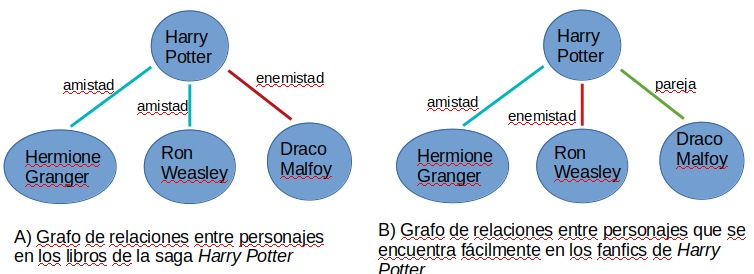
\includegraphics[scale=0.6]{rel_graph_hp2}
	\label{fig:graph_hp}
	\centering
\end{figure}


Como se ha dicho anteriormente, los fans se organizan en comunidades según la obra que es el objeto de su admiración, y tienen sitios como AO3, dedicados a alojar y compartir sus creaciones fan. Evidentemente, analizar las más de seis millones de obras existentes en AO3 es una tarea imposible con los recursos a mi alcance, de modo que elegí utilizar únicamente los fanfics basados en \textit{Good Omens}, un libro de Terry Pratchett y Neil Gaiman, en parte por mi familiaridad con esa comunidad, pero también porque tenía una cantidad de fanfics extensa pero manejable.

AO3 no es el único sitio web popular para alojar fanfiction, pero a lo largo de esta década ha desplazado a sitios como \href{http://fanfiction.net}{Fanfiction.net} y \href{https://www.wattpad.com/}{Wattpad}, y la característica que condicionó mi decisión es su extensivo sistema de etiquetas, que como se verá más adelante fue fundamental para filtrar y gestionar los datos del proyecto.

En términos legales y de derechos de autor, la mayoría de legislaciones considera el fanfiction como un tipo de obra derivada  \cite{woosh_1998} y por tanto entra dentro del \textit{fair use}.


\cleardoublepage
\section{EXTRACCIÓN DE INFORMACIÓN EN OTROS TRABAJOS}

La extracción de información es un problema que se aborda en el análisis de lenguaje natural, cuyo objetivo es ahorrar el trabajo humano de resumir y sacar conclusiones de grandes conjuntos de textos. Para lograrlo, se crean programas capaces de procesar información no estructurada, dotándoles de la habilidad de entender el significado del lenguaje humano para que resuman y saquen conclusiones a partir de grandes volúmenes de textos ya existentes y, por ejemplo, usen esa información para crear una base de datos de conocimiento automáticamente, sin tener que dedicar grandes cantidades de tiempo y esfuerzo a leerlos manualmente. Es especialmente útil en campos como la medicina y la química, para los cuales se han creado distintos modelos \cite{craven_99}\cite{manica_2019} con el objetivo de ayudar a procesar las ingentes cantidades de estudios y artículos que se publican hoy en día.


El primero de los pasos para extraer información de un texto es identificar las entidades nombradas en el mismo. Algunos sistemas, como CoreNLP \cite{corenlp_ner}, utilizan un clasificador estadístico (en particular, un campo aleatorio condicional \cite{laff_2001}) para identificar las palabras que denotan un nombre, lugar u organización. La desventaja de éstos métodos es que requieren ser entrenados con datos previamente etiquetados y listas de nombres bien conocidos (nomenclátor), por lo que también se han buscado alternativas no-supervisadas \cite{nothman_2013} y semi-supervisadas \cite{lin_2009}, pero las estrategias que echan mano del \textit{machine learning} y grandes corpus de texto etiquetado para entrenar clasificadores siguen siendo las más populares. Existen por tanto muchas soluciones distintas, algunas dotadas de extractores de características muy sofisticados compuestos por varios algoritmos entrenados para realizar tareas específicas, como capturar el contexto o incluso canonicalizar entidades \cite{wick_2009}.

La extracción de relaciones tradicionalmente se ha realizado tratando de identificar relaciones binarias, bien frase a frase o teniendo en cuenta dos o tres frases consecutivas \cite{zelenko_2003}\cite{craven_99}. Las limitaciones de este sistema no son sólo que no todos los tipos de relaciones son binarias, si no que cuanto más largo es un texto, menos probable es que ambas entidades aparezcan nombradas en una única frase, con lo que se pierde mucha información si se ignoran. Pasar a un sistema que tenga en cuenta varias frases interdependientes viene con sus propios problemas, pues las características sintácticas de una relación son muy dispersas en el texto y tratar de extraerlas automáticamente requiere de mucha memoria y muchos datos; más cuántas más frases tengas en cuenta. Sin embargo, recientemente se han creado algoritmos que identifican una relación n-aria a partir de todas las menciones en las que aparece, como el de Peng et al \cite{peng_17}, que utiliza grafos LSTM para modelar el contexto e información de cada frase y las conexiones entre ellas, logrando así beneficiarse de la interdependencia de distintas frases sin tanto coste de recursos.

Este proyecto sin embargo busca identificar relaciones de naturaleza social entre distintos personajes de ficción, con ĺo que se centrará en identificar entidades del tipo 'Persona', y buscará relaciones binarias entre ellas. 

Aunque el fanfiction no ha sido muy utilizado para realizar tareas de extracción de información, su disponibilidad online y la cantidad de metadatos asociados a cada obra ha hecho que algunos programadores los aprovechen para crear sistemas de recomendación, como \href{http://www.fanrecs.com/}{FanRecs}, aunque el principal interés parece residir en crear herramientas de descarga  (\href{https://www.ficlab.com/}{FicLab}, \href{https://www.fanfictiondownloader.net/#/home}{FanfictionDownloader}).



\cleardoublepage
\section{RECOGIDA Y LIMPIEZA DE DATOS}

\subsection{Creando un scraper para Archive of our Own}
\label{sec:recogidadatos}

En el momento en el que decidí utilizar los fanfics de \textit{Good Omens} para el proyecto, dicho libro tenía unos 22000 fanfics en \href{archiveofourown.org}{Archive Of Our Own} (AO3 para abreviar). Sin embargo, de todos esos relatos sólo me interesaban los que están en inglés y los que realmente contuvieran texto (puesto que, aunque AO3 se centra en relatos, permite alojar todo tipo de archivos multimedia).

Por suerte, AO3 fue creado con la intención específica de funcionar como archivo, por lo que tiene una herramienta de búsqueda y filtrado muy completa y sencilla de usar. Esta herramienta permite filtrar por características como título, autor, idioma y cantidad de palabras, pero su mayor utilidad viene de su sistema de etiquetado. AO3 permite a los autores añadir tantas etiquetas como quieran para que los posibles lectores puedan saber más de su obra a simple vista: temática, personajes principales, parejas en las que se centra, qué medio utiliza, si hay ilustraciones, si trata sobre un evento de la historia original particular... Las etiquetas añaden una gran cantidad de información sobre las historias a las que acompañan, y aunque no es obligatorio poner ninguna, en general los autores se preocupan de etiquetar correctamente sus obras.

AO3 tiene etiquetas específicas para indicar que una obra no es principalmente texto: \textit{'Fanart'}, para ilustraciones, y \textit{'Podfic'} para archivos de audio, así que aproveché la herramienta de búsqueda para llevar a cabo un primer filtrado que eliminara todas las obras que las contuvieran, además de todas las que no estuviesen en inglés. El resultado fue un subconjunto de 20190 fanfics, todos en inglés y cuyos autores no habían incluido ninguna etiqueta que indicara que no fuera puro texto. La herramienta además genera un link permanente que siempre lleva a este subconjunto particular, por lo que no es necesario utilizar esta herramienta nada más que una vez.

Una vez localizado el conjunto de textos y el link a los mismos, viene la parte de crear el \textit{scraper} en sí. Utilizando la herramienta de inspeccionar elemento de \textit{Firefox} para explorar la estructura del sitio, y enseguida se hizo obvio que los fanfics estaban organizados en páginas con un máximo de 20 fanfics cada una. En el HTML de la página, cada fanfic se presenta dentro de una clase llamada \textit{'work blurb group'}. No se puede extraer un link de descarga directamente de ésta clase, pero sí el identificador del fanfic.


\newpage
\begin{SCfigure}
	\caption{Herramienta de filtrado de AO3. Permite excluir (o incluir) obras que contengan etiquetas específicas, así cómo aquellas no escritas en un idioma particular}
	\label{fig:ao3_search}
	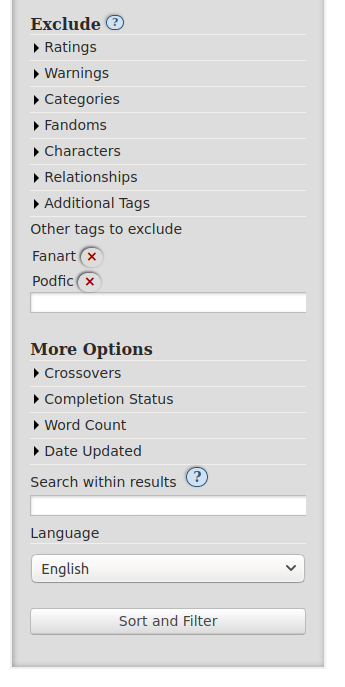
\includegraphics[scale=0.5]{ao3_searchbox}
	\centering
\end{SCfigure}


En AO3, cada fanfic tiene un número que lo identifica de forma única. Es posible acceder a la página de cualquier fanfic simplemente añadiendo ese número al final de \newline 'https://www.archiveofourown.org/works/' en la barra de direcciones, y en esa página sí que se pueden encontrar links de descarga.
Por tanto la idea básica para el \textit{scraper} es utilizar las librerías \textit{requests} y \textit{BeautifulSoup} de python para explorar los veinte \textit{'work blurb group'} de cada página, localizar el identificador de cada uno, utilizarlo para acceder a la página del fanfic y extraer el link de descarga. Y así con cada página del listado, hasta llegar a la última. La figura \ref{fig:ao3_structure} ilustra el proceso con un esquema.

\begin{figure}[h]
	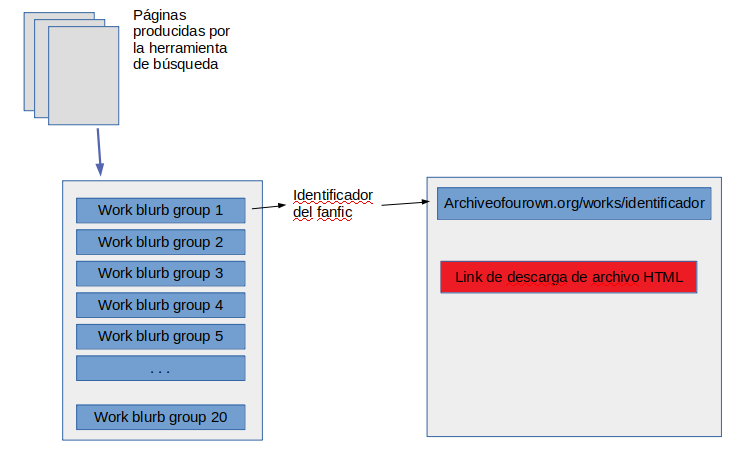
\includegraphics[scale=0.5]{ao3_structure}
	\caption{Concepto para el \textit{scraper}. El objetivo es obtener los links de descarga navegando las páginas de búsqueda.}
	\label{fig:ao3_structure}
	\centering
\end{figure}

\newpage

\begin{figure}
	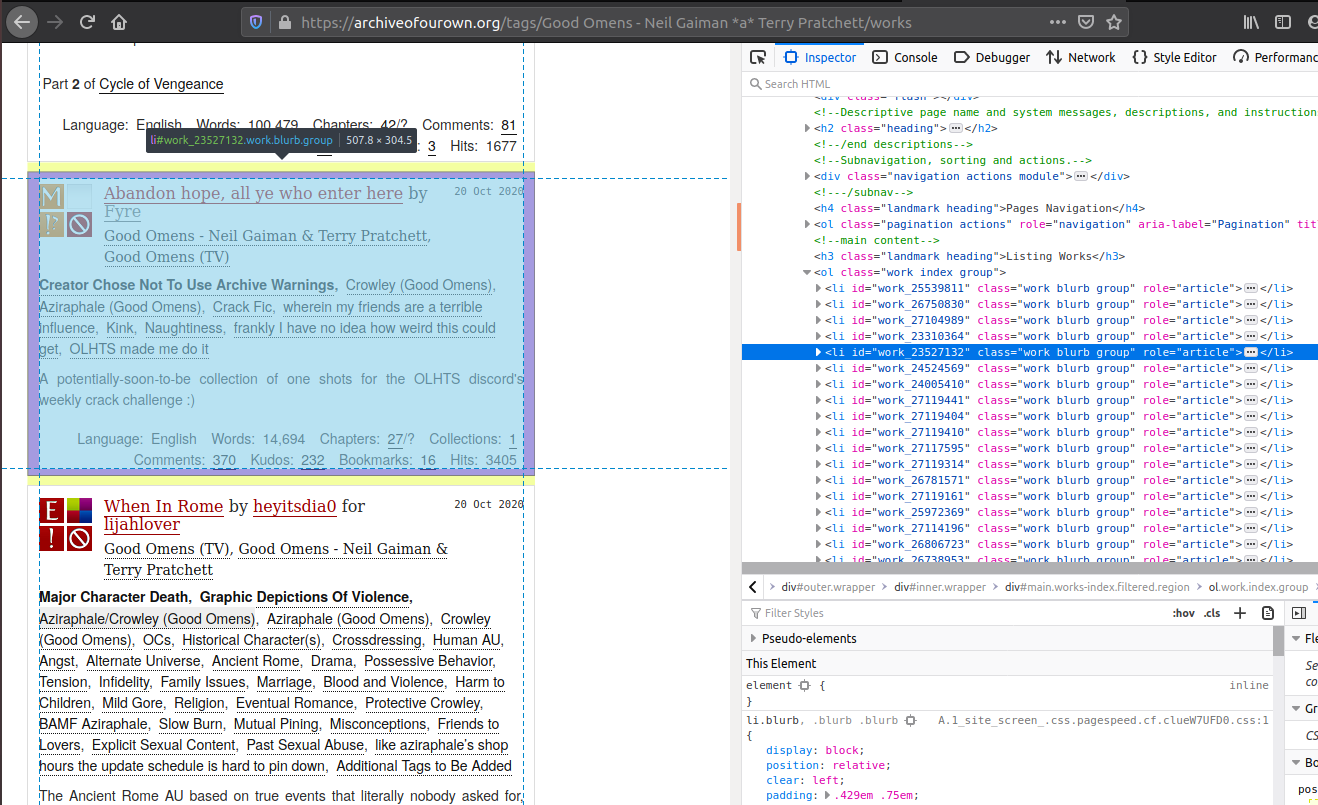
\includegraphics[angle=90,scale=0.4]{ao3_inspect}
	\caption{Exploración de la estructura de la página AO3 usando la herramienta 'Inspeccionar elemento' de \textit{Firefox}. Se puede ver que el sitio utiliza una clase HTML llamada \textit{'work blurb group'} para mostrar cada obra.}
	\label{fig:ao3_inspect}
	\centering
\end{figure} 



El proceso de descarga de archivos, en principio, tendría estos pasos:

\begin{enumerate}
	\item Enviar una petición HTTP GET al link permanente del conjunto de datos, generado por la herramienta de búsqueda de AO3.
	\item Iterar entre los 20 \textit{'work blurb group'} y extraer el identificador de cada uno.
	\item Usar el identificador para acceder a la página de cada fanfic, extraer el link de descarga de la página, y descargar el fanfic como archivo HTML. Hacer esto con los 20 identificadores.
	\item Pasar a la siguiente página y repetir, hasta llegar a la última.
\end{enumerate}

Utilizando la librería \textit{requests} de python, el primer paso es trivial, y se puede observar en la figura \ref{code:scraper1}. Encontrar los identificadores tampoco es complicado. Se puede apreciar en \ref{fig:ao3_structure} que el identificador del fanfic también es el ID del objeto \textit{'work blurb group'} al que pertenece, y expandiendo la clase se puede ver que el identificador completo se puede encontrar dentro del objeto, como un objeto de tipo \textit{h4}. Por tanto, usando \textit{BeautifulSoup} para manejar los datos resultantes de la petición HTTP GET como objeto HTML, se pueden obtener todos los objetos \textit{'work blurb group'} usando la función \textit{find(class\_=<nombre clase>)}, cuyo resultado es una lista con los 20 objetos, sobre los cuales se itera para encontrar los identificadores usando de nuevo la función \textit{find()}. En la figura \ref{code:scraper2} se puede observar un fragmento del código que realiza este trabajo; el código completo se puede consultar en \refToLinkScraperCode.

\begin{figure}
	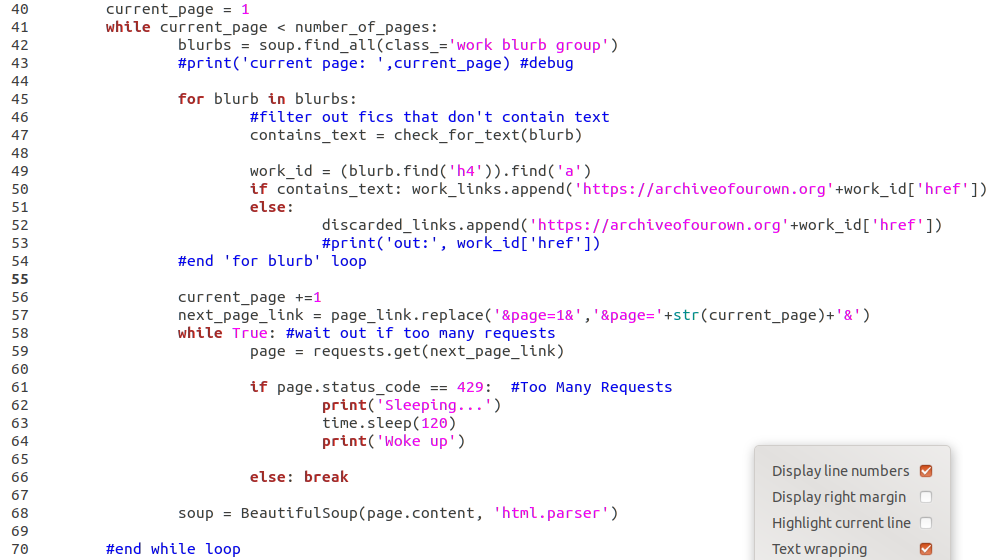
\includegraphics[scale=0.4]{scraper_code2}
	\caption{Código perteneciente al \textit{scraper} 'ao3\_link\_scraper'. Utiliza un bucle \textit{while} para iterar entre las páginas de la búsqueda, y en cada página, usa la librería \textit{BeautifulSoup} para extraer los objetos 'work blurb group' en una lista llamada 'blurbs' (línea 42). De cada 'blurb' extrae el identificador del fanfic y comprueba si tiene texto (líneas 46-49), y si lo contiene forma el enlace a la página del fanfic y lo añade a una lista llamada 'work\_links' (línea 50). Si no contiene texto, se añade a otra lista llamada 'discarded\_links' (línea 52).}
	\label{code:scraper2}
\end{figure}


Las complicaciones empiezan una vez se tienen los identificadores. Para formar la dirección completa, hay que añadir el identificador al final de \textit{'https://www.archiveofourown.org'}, mandar otra petición HTTP GET a dicha dirección, buscar ahí el link de descarga, solicitarla, esperar a que la descarga termine, y repetir todo esto otras 19 veces hasta tener descargados todos los fanfics de la página. Esto significa que por cada iteración del bucle que explora cada página es necesario introducir otro bucle que haga las descargas.

\begin{figure}
	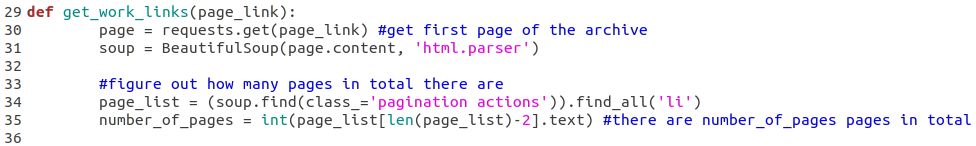
\includegraphics[scale=0.5]{scraper_code}
	\caption{Código perteneciente al \textit{scraper} 'ao3\_link\_scraper'. Utiliza la librería \textit{requests} para enviar una petición HTTP GET al link permanente del conjunto de datos (línea 30), y \textit{BeautifulSoup} para navegar el resultado como un objeto HTML del que poder extraer datos útiles, como la cantidad total de páginas (líneas 33-35).}
	\label{code:scraper1}
	\centering
\end{figure}

\begin{figure}
	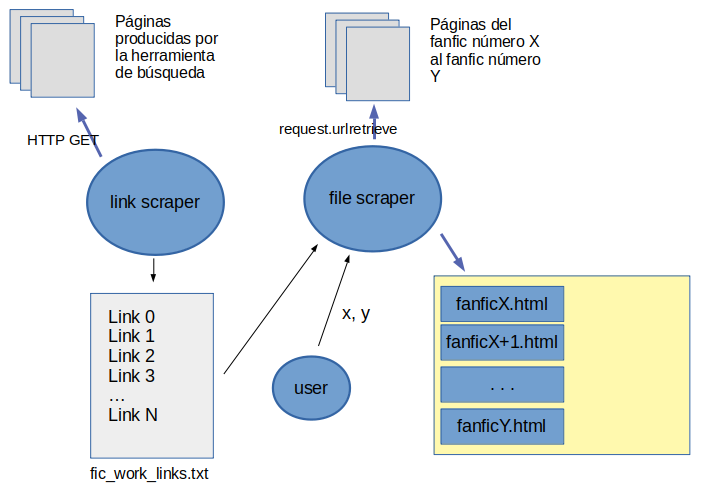
\includegraphics[scale=0.4]{scrapers_structure}
	\caption{Proceso de descarga de fanfics de AO3 utilizando los programas 'ao3\_link\_scraper.py' y 'ao3\_file\_scraper.py'.}
	\label{fig:scrapers_structure}
	\centering
\end{figure}


\begin{SCfigure}
	\caption{Navegación de páginas de búsqueda de AO3. Todos los botones vienen con su número de página, y se puede ver cuál es la última}
	\label{fig:ao3_structure2}
	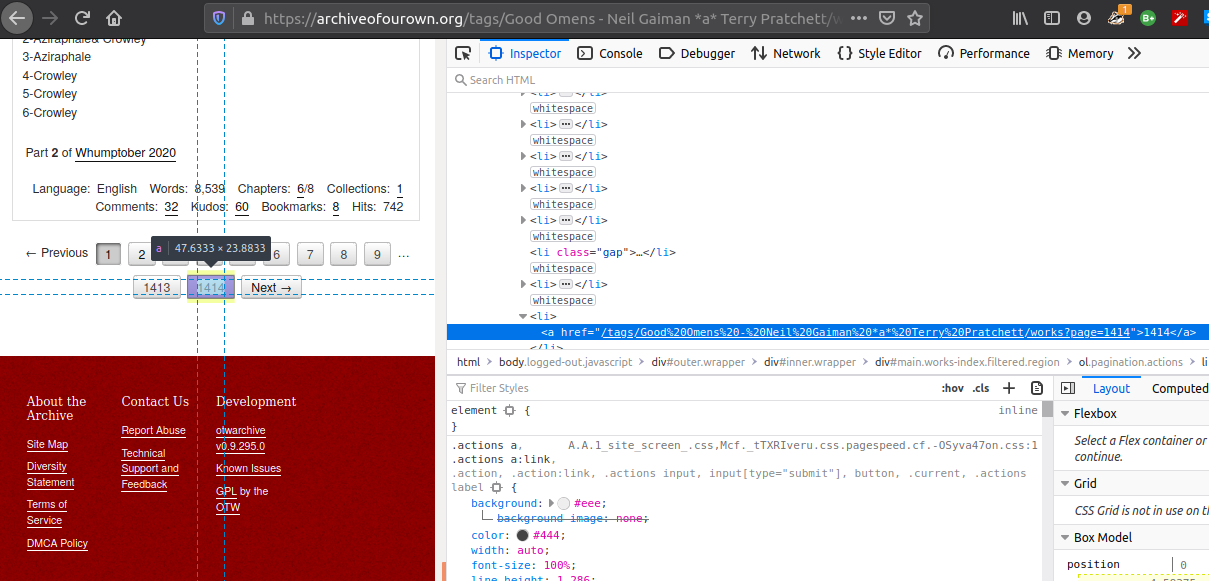
\includegraphics[angle=90, scale=0.4]{ao3_structure2}
	%\centering
\end{SCfigure}

La última parte, la de pasar a la página siguiente, es más complicada de explicar que de ejecutar. Todas las páginas de resultados de búsqueda de AO3 contienen botones para avanzar, retroceder y saltar a páginas concretas. Es posible saber cuántas páginas en total tiene la búsqueda simplemente observando el texto del botón de la última, tal y como se ve en la figura \ref{fig:ao3_structure2}. No se aprecia, pero la clase HTML a la que pertenece dicho botón se llama \textit{'pagination actions'}, y es posible extraerla gracias a la función \textit{find(class\_=<nombre\_clase>)} de \textit{BeautifulSoup}. Y ya con ese objeto, se puede volver a utilizar la función \textit{find()} para buscar todos los objetos hijos de la clase \textit{'pagination actions'} que sean de tipo \textit{li}. El último será el que contenga la cantidad total de páginas, y solicitar la siguiente consiste simplemente en sustituir la referencia en el link a la página 1 por una referencia a la última página. En la figura \ref{code:scraper1} se ve parte del código que realiza este proceso; el código completo se puede consultar en el anexo \refToLinkScraperCode.

Es evidente que la parte de solicitar las descargas en un bucle anidado ralentiza el programa, enturbia el código y además, hace que sea complicado parar o interrumpir el programa si hay algún error de red, pues para reanudar la ejecución por donde se quedó sería necesario almacenar en alguna parte el número de página por el que iba y el número del fanfic dentro de esa página, y programar los bucles para que salten directamente a la iteración deseada.

Ninguna de estas cosas me convenía, ya que descargar más de 20000 archivos ya iba a ser lento de por sí y hacerlo de una sentada sería prácticamente imposible, de modo que decidí dividir el programa en dos: uno que llamé 'link \textit{scraper}' y otro '\textit{file scraper}'.



El link \textit{scraper} se ejecutaría una vez y exploraría todas las páginas de búsqueda, extrayendo los links a los fanfics de cada una, y los almacenaría en un archivo de texto. Por tanto, al terminar su ejecución este \textit{scraper} ha generado un archivo llamado '\textit{fic\_work\_links.txt}' que almacena los enlaces a cada fanfic. El \textit{file scraper} utiliza esta lista para saber dónde buscar las descargas, y el usuario le indica en la línea de comando los índices que acotan el tramo de la lista a descargar, tal y como se ilustra en el esquema de la figura \ref{fig:scrapers_structure}. De este modo, es posible indicarle al programa que descargue desde el link 0 al link 1000 de la lista, permitiendo descargar los 20000 archivos en porciones manejables. Además, el programa anuncia en pantalla qué link está siendo descargado en cada momento, por lo que si sucede un error de red mientras descargaba el link número 866, es posible reanudar el programa fácilmente e indicarle que continúe desde el 866 al 1000.

Esta división del trabajo en dos programas además me daba la oportunidad de introducir con sencillez un segundo filtrado durante el proceso de exploración que realiza el link \textit{scraper}. Si el primer filtrado se encargaba de cribar los fanfics que habían sido etiquetados por sus autores como imágenes o audio, este segundo filtrado pretende detectar los fanfics que tampoco contienen texto, pero no han sido etiquetados como tal por sus autores. Para ello usé el criterio de la relación palabras/capítulo de cada fanfic: si una obra tiene menos de 40 palabras por capítulo, se considera como fanfic "sin texto", y se elimina. Escogí 40 palabras como umbral tras investigar un poco con la herramienta de búsqueda de AO3, que como se puede ver en la figura \ref{fig:ao3_search}, tiene una opción para filtrar por cantidad total de palabras. Tras probar varios umbrales, 40 parecía ser el que descartaba todas las obras sin texto sin sacrificar muchos microrrelatos en el proceso.

Introducir este filtrado en el \textit{scraper} fue sencillo, puesto que el número de palabras y capítulos de la obra es información que se puede extraer de la clase \textit{work blurb group} de cada fic. Todo esto se realiza desde la función \textit{check\_for\_text}, y en la figura \ref{code:scraper2} se puede ver cómo el bucle llama a dicha función; el código completo se puede consultar en \refToLinkScraperCode. Por tanto, el link \textit{scraper} realiza estos pasos:
\begin{enumerate}
	\item Enviar una petición HTTP GET mediante la librería \textit{requests} al link permanente del conjunto de datos, generado por la herramienta de búsqueda de AO3.
	\item Iterar entre los 20 \textit{'work blurb group'}, comprobar si contienen texto, y descartar los identificadores de los que no.
	\item Utilizar cada identificador para generar el link de la página de cada fanfic y almacenarlos en un archivo de texto.
	\item Pasar a la siguiente página y repetir, hasta llegar a la última.
\end{enumerate}

Por su parte, el \textit{file scraper} realiza estos pasos:
\begin{enumerate}
	\item Abrir el archivo \textit{fic\_work\_links.txt} y extraer la lista de links.
	\item Mediante la librería \textit{requests}, realizar una petición HTTP GET al primer link, saltando al siguiente si devuelve un código 404.
	\item Extraer el link de descarga HTML de cada página.
	\item Solicitar la descarga mediante \textit{request.urlretrieve}. Guardar el archivo resultante en la carpeta adecuada en el sistema.
	\item Repetir con todos los links de la lista.
\end{enumerate}

El manejo del código de error 404 (Page Not Found) es bastante importante en este \textit{scraper}, puesto que entre el momento en el que se almacenó el link del fanfic mediante el primer \textit{scraper} y el momento en el que el segundo \textit{scraper} lo utiliza para la descarga pueden haber pasado varios días. En ese tiempo, el autor del fanfic puede haber decidido borrar el fanfic de AO3, o haberlo hecho privado, y de ahí que el \textit{scraper} reciba un 404. Un simple \textit{try-catch} detecta el código 404 y simplemente pasa al siguiente link, como se puede consultar en el anexo \refToFileScraperCode.

El otro error que ambos \textit{scrapers} necesitaban manejar es, naturalmente, el error 429 (Too Many Requests). En las líneas 58-66 de la figura \ref{code:scraper2} se puede ver cómo se utiliza un \textit{try-catch} que envuelve la petición HTTP GET para detectar el status 429 y, en vez de pasar al siguiente link, se lanza una espera de dos minutos tras la cual vuelve a solicitar la página. Antes de incorporar este código a los \textit{scrapers} creé un pequeño programa de prueba, para ver cuánto tardaba AO3 en enviar un 429 y cuánto tiempo de espera requería antes de volver a aceptar solicitudes.
 
%Decidí dividir este proceso en dos programas (el de navegación y filtrado, y el que únicamente descarga) en vez de hacerlo todo en uno porque descargar los más de 20000 archivos de una vez lógicamente tardaría varias horas, y pensé que sería más pragmático si ejecuto una vez el \textit{scraper} crea una lista de enlaces, y luego ya ejecuto todas las veces que sean necesarias el \textit{scraper} que descarga, descargando cada vez un tramo distinto de la lista. De esta forma, pude descargar todos los fanfics en grupos de 2000 (alrededor de una hora y media), pudiendo tener el ordenador libre el resto del tiempo.

El resultado de la ejecución de estos \textit{scrapers} es una carpeta con 818,8 MB de archivos HTML.

\begin{figure}[h]
	\centering
	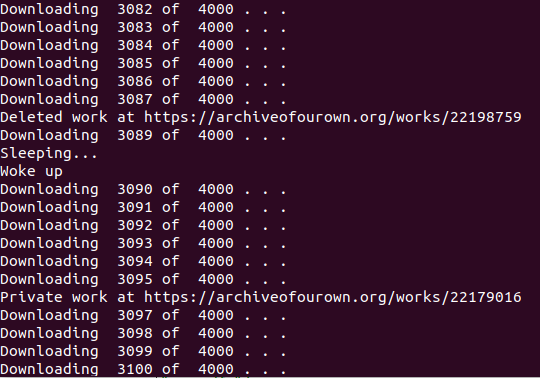
\includegraphics[scale=0.5]{ejecucion_file_scraper}
	\label{fig:file_scraper}
	\caption{Ejecución de \textit{ao3\_file\_scraper.py}}
\end{figure}


\subsection{Limpieza de datos y creación de datasets}
\label{sec:limpiezadatos}

Al terminar el proceso de descarga, acabé con un conjunto de archivos HTML y un archivo TXT con una lista de los \textit{path} de todos ellos.

La principal tarea de limpieza de datos es, por tanto, convertir los archivos HTML a texto. Para ello utilicé la librería \textit{HTML2Text}, que como cuyo nombre dice sirve para eso mismo. Sin embargo, los fanfics en HTML no contienen sólo el texto del fic en sí, sino que también contienen todos los metadatos del mismo: etiquetas, \textit{rating}, resumen, comentarios del autor, entre otros, con lo que tras limpiar el archivo HTML con \textit{HTML2Text} el resultado no era el texto puro del fanfic. Tuve que crear varias funciones y ayudarme de \textit{Beautiful Soup} para limpiar todos estos metadatos y dejar únicamente el texto en sí, sin llevarme por delante parte del texto ni dejarme notas del autor entre capítulos.

Al principio puse estas funciones dentro de cada programa que necesitaba manejar los textos, pero obviamente enseguida se volvió muy aparatoso, por lo que consolidé todas las funciones de limpieza en un único archivo, \textit{fanfic\_util.py}, junto con tres clases para encapsular el uso de estas funciones:

\begin{itemize}
	\item FanficGetter, que se encarga de proveer el texto limpio de un fanfic (o lista de fanfics) a demanda. Al principio devolvía los textos como una lista de \textit{string}, pero luego resultó más útil que devolviera una lista de objetos \textit{Fanfic} que pudiera devolver los capítulos por separado o juntos en un mismo \textit{string}, además del identificador del fanfic.
	\item FanficHTMLHandler se encarga de extraer información de los metadatos del archivo HTML de un fanfic, como por ejemplo los personajes principales, las relaciones, las etiquetas, el número de capítulos y su clasificación.
	\item Fanfic, una clase que se utiliza a lo largo del proyecto para encapsular toda la información relevante sobre un fanfic, como sus capítulos, sus personajes, etiquetas, el dataset al que pertenece e incluso los objetos \textit{Document} generados por CoreNLP.
\end{itemize}

La creación de la clase \textit{Fanfic} surgió a mediados del proyecto, cuando el límite de 100000 caracteres de \textit{CoreNLP}\ref{nota:limiteCarac} hizo necesario poder acceder al texto de cada fanfic dividido en capítulos. \textit{Fanfic} por tanto tiene un atributo \textit{chapters}, que es la lista de \textit{string} con los capítulos, y un método \textit{get\_string\_chapters()} que devuelve todos los capítulos en un único \textit{string}. Según seguía avanzando la clase también demostró ser útil para almacenar en un único elemento toda su información relevante, por lo que termina siendo la unidad básica de trabajo del proyecto.

\begin{figure}[h]
	\centering
	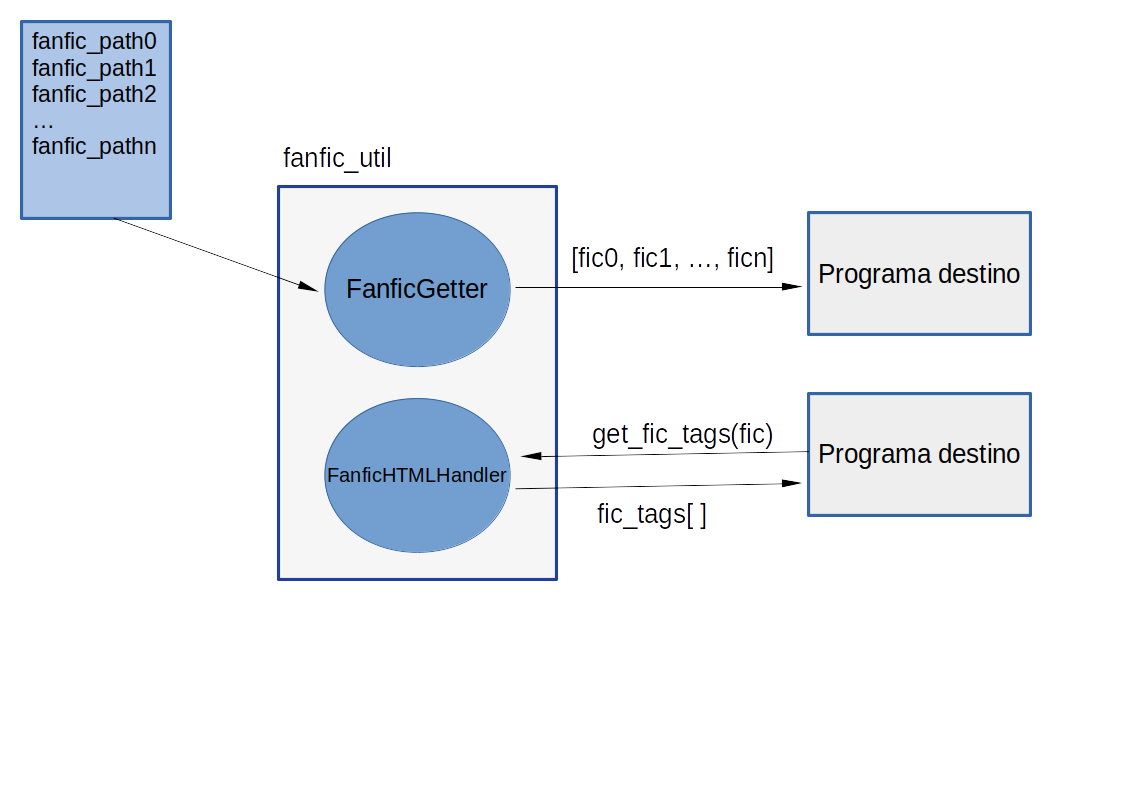
\includegraphics[scale=0.4]{fanfic_util_functions}
	\caption{Esquema ilustrando la función de las clases \textit{fanfic\_util}}
	\label{fig:fanfic_util}
\end{figure}

Sin embargo, el acceso a los datos sigue basándose en una lista de \textit{paths} guardada en un archivo TXT. Es un sistema muy rudimentario (ilustrado en la figura \ref{fig:fanfic_util}), pero no vi necesidad de trasladarlo a una base de datos propiamente dicha, puesto que nada en la creación de una base de datos me ahorraba nada del trabajo de crear \textit{fanfic\_util}, y desde el punto de vista del resto de programas es igual acceder al texto de un fanfic a través de FanficGetter que de una función que recupere el texto de una base de datos. Únicamente intercambiaría el tiempo de limpiar los textos por el de conectar con la base de datos y extraer su información.

El identificador de entidades puede utilizar la lista original con todos los fanfics como fuente para etiquetarlos, pero para la parte de identificación de relaciones del proyecto se necesita filtrar los fanfics originales en tres subconjuntos: uno centrado en el romance, otro en la amistad, y el último en la enemistad. Por lo tanto, utilicé las funciones de \textit{fanfic\_util} para crear un programa, \textit{generate\_fic\_lists.py}, para crear las listas de \textit{paths} correspondientes a cada grupo.

El criterio utilizado para crear estos tres grupos está basado en la longitud de los textos y sus etiquetas. En el caso de las etiquetas es sencillo: los autores casi siempre etiquetan las relaciones románticas en sus relatos, y a menudo también las amistades, para hacer que sus historias sean más fáciles de encontrar por aquellos que quieran leerlas. En AO3, las etiquetas románticas tienen el formato 'Personaje A/Personaje B', mientras que las etiquetas de amistad son 'Personaje A \& Personaje B' o 'Personaje A and  Personaje B', con lo que extraer estas etiquetas del archivo HTML es sencillo utilizando expresiones regulares. Además de tener una etiqueta que valide la expresión regular, sólo tuve en cuenta aquellos relatos que sólo tenían un capítulo. De esa forma, esperaba poder eliminar historias largas y elaboradas que contienen romance, pero que principalmente son una historia costumbrista o de aventuras. Limitando la longitud de la historia a un capítulo, todo el romance o la amistad queda condensada en dicho capítulo. Además, como en los relatos que contienen abusos sexuales es común etiquetar al perpetrador y a la víctima con el formato de 'Personaje A/Personaje B', realicé un segundo pase a la lista de romance, eliminando todos aquellos relatos que tuviesen la etiqueta 'Rape/Non-con'.

Crear un conjunto con relaciones de enemistad u odio es una tarea más complicada, ya que los usuarios de AO3 no tienen un formato oficial para las mismas y no se suelen etiquetar. Al final utilicé una lista de las etiquetas que los autores comúnmente utilizan como aviso de que su historia contiene violencia o abusos, como 'Rape/Non-con', 'Torture', 'Graphic Depictions of Violence' o 'Dead Dove: Do Not Eat'. Esperaba que, entre esas etiquetas y la limitación de longitud, pudiese aislar un conjunto de relatos que sirvieran de modelo para la relación de enemistad.

El resultado fueron 12520 relatos en el conjunto de romance, 784 en el de amistad y 155 en el de enemistad. Para equilibrar los \textit{datasets}, reduje el conjunto de romance a 220 y el de amistad a 180, dando un total de 555 relatos para modelar estas relaciones. A este \textit{dataset} lo llamo 'RFE dataset' (por \textit{Romance, Friendship, Enemy}) y se utiliza en la sección \ref{sec:relextract}.

\cleardoublepage
\section {EXTRACCIÓN DE DATOS A PARTIR DE TEXTO}

En la identificación de entidades, se considera una entidad a los personajes, los lugares y las instituciones, entre otras cosas, que haya sido nombrada en el texto. Un algoritmo capaz de identificar entidades nombradas tiene que poder dividir un texto en tramos y asignarle una etiqueta de entidad ("Persona", "País", etc) a cada uno. Esta tarea además requiere que las palabras del texto hayan sido previamente etiquetadas con su rol morfológico.

Por estos motivos, la librería NLTK parecía la más idónea para la tarea. Es una librería de python que contiene herramientas básicas para el análisis de texto, y en particular me interesaba que venía con un \textit{part of speech tagger} (es decir, un identificador de rol morfológico) ya programado y entrenado. NLTK también viene con un identificador de entidades ya entrenado, pero quería programar uno que fuera más preciso y adaptado a mi conjunto de datos.



\subsection{Algoritmo de identificación de entidades}

\subsubsection{Extracción de entidades con NLTK}
\label{sec:nerextract_tagger}
Además del identificador de rol morfológico, NLTK también tiene una clase llamada \textit{ChunkParser} cuyo trabajo es dividir un texto en tramos. Todas las funciones de la librería que se encargan de dividir y/o etiquetar texto (como el identificador de rol morfológico) heredan de alguna versión de la clase \textit{ChunkParser}, de modo que la idea para el algoritmo era modificar la clase \textit{ChunkParserI} para convertirla en un identificador de secuencias basado en características. El código utilizado en este proyecto está basado en el tutorial de Ivanov en \textit{Natural Language Processing for Hackers} \cite{ivanov_2016}.

Un identificador de secuencias basado en características trata de asignar un peso a un tramo concreto, y según el peso, le asigna una etiqueta u otra. Este peso se calcula como una función de las características del propio tramo, así como de los tramos que le preceden.
El programador puede elegir las características que considere más importantes, pero hay algunas que son bien conocidas como las más importantes para reconocer entidades, como:

\begin{itemize}
	\item El rol morfológico de la palabra actual, las anteriores y las siguientes.
	\item La forma de la palabra, las anteriores y las siguientes (si empiezan por mayúscula, si tienen signos de puntuación, si son siglas, etc)
	\item Los prefijos y/o sufijos de la palabra actual, las anteriores  y las siguientes.
	\item Si la palabra anterior ha sido identificada como una entidad o no.
	
\end{itemize}

El conjunto de características de cada tramo se llama vector de características, y se utiliza para calcular un "peso" que se corresponde con la probabilidad de que un tramo X con un vector de características V tenga una etiqueta Y. El algoritmo al final asigna a cada tramo la etiqueta cuyo peso sea el más alto.

El cómo se calcula exactamente ese peso depende del modelo matemático a utilizar. A la versión modificada de ChunkParserI para la identificación de entidades la llame NERChunker (NER por Named Entitiy Recognition), y tiene tres versiones:

\begin{itemize}
	\item NERChunkerv1 y NERChunkerv3 utilizan un modelo de regresión logística (también llamado modelo de entropía máxima), a través de la clase MaxentClassifier de NLTK. Para que NLTK pueda utilizar esta clase correctamente, es necesario tener instalado el módulo Megam para python, que no viene incluído en NLTK. La única diferencia entre la versión 1 y la 3 de este chunker es que la 3 maneja las estructuras de NLTK para oraciones y etiquetas de forma ligeramente más rápida.
	\item NERChunkerv2, que utiliza un modelo de naïve Bayes a través de la clase ClassifierBasedTagger de NLTK.
	
\end{itemize}

Las versiones \textit{v1} y \textit{v3} de \textit{NERChunker} obtuvieron los mejores resultados en la evaluación, y la \textit{v3} es algo más rápida, por lo que es la versión definitiva del identificador de entidades. Todas estas versiones, junto con sus funciones auxiliares, se encuentran encapsuladas en el archivo \textit{NERChunkers.py}, para ser utilizadas donde se las necesite.

Puesto que tanto los clasificadores de regresión logística como los de \textit{naïve} Bayes son algoritmos de aprendizaje supervisado, antes de poder utilizar (o evaluar) cualquiera de las versiones de \textit{NERChunker} era necesario entrenarlas con un conjunto de datos ya etiquetados. El problema aquí es que NLTK, a pesar de incluir un corpus muy extenso en la propia librería, sólo tiene dos conjuntos de datos para identificación de entidades: uno en español y el otro en holandés. Todos los textos a analizar en el proyecto están en inglés, obligándome a buscar un conjunto ajeno a NLTK y finalmente decidiéndome por \textit{Groningen Meaning Bank} (GMB). GMB es un \textit{dataset} para identificación de entidades específicamente en inglés, grande, con una gran variedad de etiquetas de entidad y, sobretodo, con un formato de etiquetado sencillo de entender,cosa importante puesto que al ser ajeno a NLTK, GMB utiliza etiquetas distintas que son necesario adaptar para que \textit{MaxentClassifier} pueda trabajar con ellas.

GMB utiliza la notación IOB para etiquetar entidades, y separa cada palabra de la siguiente por un carácter de nueva línea, y cada frase, por dos. De modo que la frase \textit{"Mr. Blair left for Turkey Friday from Brussels."} en GMB tendrá el aspecto de la figura \ref{fig:tags1}.

\begin{figure}[h]
	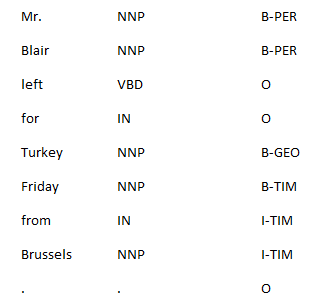
\includegraphics[scale=0.9]{GMB_tag}
	\caption{Frase etiquetada por GMB. De izquierda a derecha, las columnas representan la palabra a etiquetar, la etiqueta de rol morfológico, y la etiqueta IOB.}
	\label{fig:tags1}
	\centering
\end{figure}

Cuando el programa detecta una entidad de tipo persona, etiqueta como 'B-PER' la primera palabra de la secuencia, mientras que el resto de palabras dentro de la secuencia son etiquetadas como 'I-PER'. Similarmente, si la entidad es de tipo geográfico las etiquetas usadas serán 'B-GEO' y 'I-GEO', si es de tiempo serán 'B-TIM' y 'I-TIM', etc. Si una palabra no forma parte de ninguna secuencia de entidad, se etiqueta como 'O'.

NLTK, por su parte, no utiliza la notación IOB  ni caracteres de nueva línea, sino que utiliza una estructura de datos propia de tipo árbol que encapsula cada palabra y cada tramo con su etiqueta. La misma frase etiquetada por NTLK tiene el aspecto de la figura \ref{fig:tags2}.

\begin{figure}[h]
	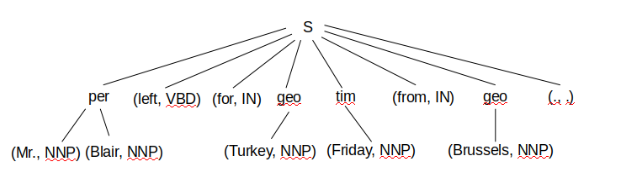
\includegraphics[scale=0.8]{NLTK_tag}
	\caption{Frase etiquetada por NLTK. Las etiquetas de entidad se encuentran en los nodos, encontrándose todas las palabras pertenecientes a una secuencia de entidad en la profundidad 2 del árbol. Las palabras que no pertenecen a ninguna secuencia de entidad se encuentran en la profundidad 1. Cada hoja del árbol contiene una tupla formada por la palabra y su etiqueta de rol morfológico.}
	\label{fig:tags2}
	\centering
\end{figure}

Como se ve, en vez de usar etiquetas IOB, NLTK organiza las palabras y su etiquetas en una estructura de árbol. La raíz, S, indica el inicio de la frase (Sentence), y las etiquetas de entidad son nodos.

En horizontal queda así:

(S, [(per, [(‘Mr.’, NNP), (‘Blair’, NNP)]), (‘left’, VBD), (‘for’, IN), (geo, [(‘Turkey’, NNP)]), (tim, [(‘Friday’, NNP)]), (‘from’, IN), (geo, [(‘Brussels’, NNP)]), (‘.’,.)])

Fue más o menos a estas alturas del proyecto cuando decidí separar el proceso de entrenar el identificador de entidades y el de utilizarlo para etiquetar texto nuevo en dos programas distintos (NERTrainer y NERTagger, respectivamente). Acceder a los textos de GMB y transformar sus etiquetas a un formato que NLTK pueda entender y acceder a los textos de la base de datos de fanfics y preprocesarlos para su posterior etiquetado mediante el programa ya entrenado han resultado ser dos procesos muy distintos, y dividirlo parecía la mejor manera de tener un código limpio y claro.

Por lo tanto, el programa \textit{NER\_trainer.py} se encarga únicamente de entrenar el \textit{chunker} y guardarlo en un objeto binario con la ayuda de \textit{pickle}, mientras que el programa \textit{NER\_tagger.py} carga el objeto binario y lo encapsula en una clase NERTagger. Cuando otro programa quiere usar NERTagger, sólo tiene que importarlo y usar su función \textit{parse(text)}, que requiere el texto completo a analizar, previamente etiquetado con el rol morfológico de cada palabra. En este aspecto, funciona de forma parecida al resto de \textit{taggers} de NLTK.

\begin{figure}
	\centering
	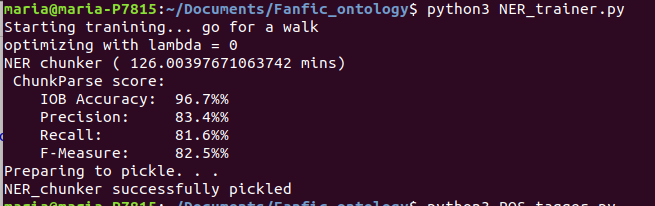
\includegraphics[scale=0.6]{ejecucion_nertrainer}
	\caption{Ejecución final de \textit{NER\_trainer.py}, mostrando su evaluación.}
	\label{fig:ner_evaluation}
\end{figure}

Sin embargo, al contrario que los modelos de NLTK, NERTagger no devuelve el texto entero con los personajes etiquetados en objetos tipo árbol, sino que devuelve directamente la lista con los nombres de los personajes y el número de veces que es mencionado cada uno. Además, tras la extracción de personajes el programa realiza una canonicalización de personajes.

Vamos a aprovechar el hecho de que los relatos que estamos manejando pertenecen al género fanfic, es decir, son obras basadas en obras ya existentes. Eso quiere decir que hay una alta probabilidad de que la mayoría o incluso todos los personajes del fanfic no sean creación del autor, sino que ya aparecían en la obra original. A estos personajes se les llama 'personajes canon'.

En este proyecto, la canonicalización de personajes consiste en descubrir qué personajes del fanfic son canon o no. Para ello necesito la lista de personajes que sí que son canon, de modo que, con la ayuda de \href{https://goodomens.fandom.com/wiki/Category:Characters}{la página de personajes de la wiki de \textit{Good Omens}}\footnote{https://goodomens.fandom.com/wiki/Category:Characters}, creo un archivo llamado \textit{canon\_characters.csv} que sirve como base de datos de los personajes de la obra original, asignándole a cada uno un identificador numérico. La base de datos además también contiene el género canónico de cada personaje, y una lista con sus apodos.

Usando la base de datos es sencillo comprobar si un personaje pertenece al canon simplemente observando si su nombre o parte de su nombre coincide con el nombre o algún apodo de un personaje canon. Para no pasar por alto posibles erratas cometidas por los autores al escribir, se considera que dos nombres coinciden cuando la distancia de edición \cite{levenshtein_1966} entre ellos es menor que una distancia máxima, cuyo valor se depende de lo largos que sean los nombres. Por ejemplo, un candidato a personaje llamado 'Azriaphale' será enlazado con el personaje canon 'Aziraphale', mientras que para que un candidato sea enlazado con 'War' o 'God' la distancia de edición tendrá que ser 0, puesto que son nombres muy cortos e incluso una distancia de edición de 1 añadiría ruido como 'dog', 'Got', 'warm' o 'ware'. Nombres que tengan varias palabras, como 'Mr. Anderson' y 'Jane Austen', se comparan palabra a palabra con los nombres de los personajes canon, y se escoge la menor distancia de edición.

El resultado final es un diccionario que incluye el nombre del personaje, el identificador numérico de su personaje canon (si lo tiene) y su número de menciones. Un ejemplo se puede observar en la figura \ref{fig:nerextract_tagger}.

\begin{figure}
	\centering
	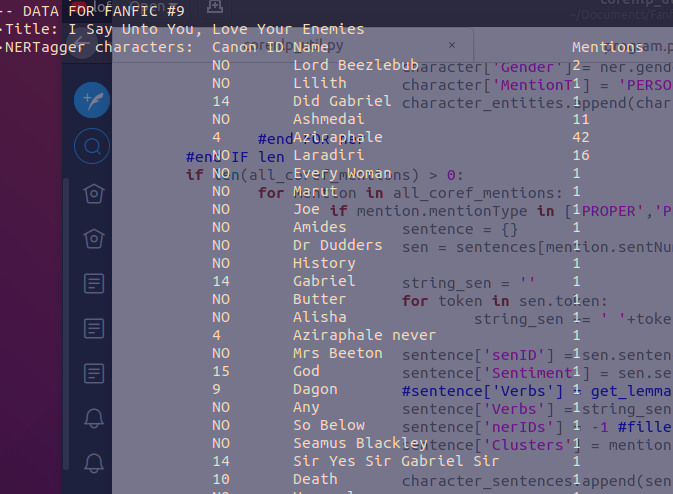
\includegraphics[scale=0.5]{nerextract_tagger}
	\caption{}
	\label{fig:nerextract_tagger}
\end{figure}
%%% DETALLES TÉCNICOS %%%
% POS\_tagger.py: para poder etiquetar las entidades nombradas es necesario etiquetar cada palabra con su rol morfológico, de modo que este programa se encarga de abrir los archivos html, pasarlos a texto y ponerle sus etiquetas morfológicas. Para ello utiliza los métodos de NLTK word\_tokenize y sent\_tokenize para dividir cada texto en frases y palabras, y pos\_tag para usar el clasificador por defecto de python para asignar etiquetar morfológicas en inglés. Almacena el resultado en un csv, de modo que en vez de tener preparar el archivo html y etiquetarlo cada vez que quiera identificar entidades, sólo tengo que etiquetar cada archivo una vez.
% NER\_trainer.py: entrena el algoritmo identificador de entidades usando el dataset de entrenamiento (descargado de aquí) y guarda el objeto en un archivo binario usando la librería pickle. Una vez entrenado, evalúa la precisión del algoritmo y la imprime por pantalla. Como el dataset no es parte del corpus nativo de NLTK, mucho de éste programa consiste en abrir el csv del dataset y empaquetar sus datos en listas y tuplas que sean compatibles con NLTK, y dividir el resultado en un dataset de entrenamiento y dos para hacer test (80\%, 10\% y 10\% del dataset original, respectivamente). Este programa utliza un objeto de la clase NERChunkerv1, que se encuentra en el archivo NER\_chunker.py, que se explica más abajo.
% NER\_tagger.py: utliza la libraría pickle para deserializar el archivo binario entrenado por NER\_trainer.py, y lo utiliza para etiquetar entidades nombradas en frases (usando etiquetas IOB). Utiliza el archivo csv creado por POS\_tagger para saltarse la parte de asignar etiquetas morfológicas, y guarda sus etiquetas en otro csv, de modo que gran parte de su código se dedica a lidiar con abrir, leer y actualizar archivos csv.


%En NERChunkerv1 he utilizado una interfaz de NLTK llamada ChunkParserI. Tiene el constructor y dos métodos:
%\begin{itemize}
%	\item el constructor recibe el dataset en forma de frases etiquetadas y entrena el algoritmo. El dataset que he utilizado venía con etiquetas IOB en forma de tuplas, pero NLTK usa las etiquetas IOB en otro formato, de modo que el constructor se dedica principalmente a manipular las tuplas y aplicarles el método tree2conlltags para que NLTK las entienda. Y después llama a NERTagger y le pasa el dataset ya preparado para entrenar un clasficador.
%	\item parse, que es el método que recibe una frase con etiquetas morfológicas y la etiqueta, con el clasificador ya entrenado. Devuelve la frase etiquetada con etiquetas IOB en forma de árbol, que es el formato de etiqueta que NLTK utiliza.
%	\item evaluate, que evalúa la precisión del algoritmo. Uso el de laIdentificación de eventos superclase, así que en mi código no está definido.
%\end{itemize}


%NERTagger mantiene un historial de etiquetas IOB (una lista) y depende de feature\_function, una función que recoge ciertas características (featureset) de una palabra y las devuelve en forma de diccionario. Las características que recoge son éstas:

\subsubsection{Extracción de entidades con CoreNLP}
\label{sec:nerextract_corenlp}
La decisión de incluir CoreNLP en el proyecto está motivada por la posibilidad de no sólo aprovechar sus capacidades para identificar menciones a una entidad en un texto, y, sobretodo, su función de resolución de correferencia para identificar relaciones entre personajes en un texto. En la sección \ref{sec:correferencia} está explicado en mayor detalle por qué esto podría ser relevante para el proyecto y cómo utilizarlo en python, pero aquí baste con mencionar que la resolución de correferencia es un método por el cual se enlaza un pronombre con el nombre propio al que se refiere. Por ejemplo, en una frase como \textit{'I love you, Juliet'} se podría aplicar correferencia para enlazar el \textit{you} con \textit{Juliet}. En este ejemplo, \textit{you} es una mención pronominal, mientras que \textit{Juliet} es una mención propia.

Esto hace que CoreNLP sea una un complemento atractivo al NERtagger desarrollado en la sección anterior, ya que además del nombre del personaje también recoge información de sus pronombres, posibilitando identificar su género y llevar una cuenta más precisa de cuántas veces se menciona un personaje concreto en el texto (incluso aunque la mención sea sólo un pronombre como \textit{he}). En esta sección se explica cómo utilizar todas estas funciones, además de los metadatos a nuestra disposición, para identificar y extraer el nombre y el género de los personajes presentes en un texto. Además, puesto que la intención del programa es que el fanfic se pueda comparar con el texto original en el que se basa, por cada personaje se identificará si aparece en la obra original o es un añadido del autor fan.

La idea básica para la extracción de personajes es buscar tanto las menciones de entidad como las de correferencia (en particular, las menciones pronominales y propias).
Como se explica en su \href{https://github.com/stanfordnlp/stanza/blob/master/doc/CoreNLP.proto}{documentación}\footnote{https://github.com/stanfordnlp/stanza/blob/master/doc/CoreNLP.proto}, CoreNLP tiene dos tipos de menciones:
\begin{itemize}
	\item \textit{NERMention}, para las menciones relacionadas con identificación de entidades. Hay varios tipos, pero este proyecto se utiliza sobretodo las menciones de tipo 'PERSON'. Cada mención tiene un entityMentionIndex que la identifica de forma única, y además también tiene un canonicalEntityMentionIndex que identifica a la entidad particular a la que hace referencia (de modo que si una entidad se llama John Smith, todas las menciones que contienen John irían idexadas a una única NERMention).
	\item \textit{Mention}, para las menciones de correferencia. En este proyecto se utilizan sobretodo las de tipo 'PROPER' y 'PRONOMINAL', ya que son las que identifican nombres y pronombres. Cada una tiene un mentionID que la identifica de forma única, además de un corefClusterID y un goldenCorefClusterID que indican los clusters a los que pertenecen.
\end{itemize}

Una vez procesado un texto, CoreNLP devuelve un objeto \textit{Document} que contiene todos los NERMention y Mention detectados en el texto. Es sencillo hallar los personajes simplemente creando una lista que contenga todas las NERMention con un mismo canonicalEntityIndex, pero todas estas menciones contienen el nombre o parte del nombre de un personaje, y mi intención era hallar también los pronombres utilizados para referirse a un personaje. Ahí es donde entra la función de resolución de correferencia, cuyo resultado se almacena en las Mention: una mención de tipo PROPER contiene el nombre de un personaje, mientras que las de tipo PRONOMINAL contienen algún pronombre. CoreNLP organiza todas estas menciones en clusters, de modo que una mención PROPER y una mención PRONOMINAL comparten el mismo cluster si se refieren a la misma entidad. Para decidir en qué cluster debe ir una mención, CoreNLP tiene en cuenta factores como el género identificado de la entidad, la distancia entre menciones y cuál fue la última entidad mencionada.

La estrategia más evidente es hacer una lista con todas las menciones PROPER y PRONOMINAL, identificar sus clusters y asociarlos a las entidades de las NERMentions, de modo que por cada texto se tenga una lista de personajes únicos con su identificador, su nombre y su género.

Sin embargo, antes incluso de empezar a entender cómo se relacionan las Mention y NERMention con el texto, hay que tratar el problema de la latencia de CoreNLP, y es que es un servidor que realmente no está preparado para procesar grandes cantidades de información. Mis primeros programas manejando CoreNLP podían tardar alrededor de un minuto por texto, lo cual no es un problema terrible para procesar uno o dos textos, pero puesto que la intención inicial de utilizar CoreNLP era analizar un dataset de casi 400 textos (sección \ref{sec:correferencia}) me vi obligada a buscar una forma eficiente de realizar las peticiones. Además, muchos de los textos exceden el límite de 100000 caracteres del servidor, lo cual hace que la petición expire y el servidor se cierre, terminando el programa. Aunque es posible aumentar dicho límite con los parámetros de configuración del servidor, la mejora en rapidez es insuficiente.

El límite de caracteres tiene fácil solución, puesto que basta con enviar cada fanfic como una lista de capítulos \label{nota:limiteCarac} (dividiendo aquellos que aún sigan excediendo el límite), y cada capítulo se envía en un petición separada. Obviamente eso significa que por cada texto se pueden recibir dos o más objetos \textit{Document}, lo que significa que un mismo personaje puede tener distintos identificadores según el \textit{Document} en el que se generó su mención, lo que complica ligeramente el proceso de consolidación de personajes, como se explica más adelante. Sin embargo, esta división del texto en distintas peticiones evita con éxito que expiren por ser demasiado grandes, pero la respuesta sigue siendo muy lenta para listas de más de 9 ó 10 textos, dependiendo de lo largos que sea cada uno.
Finalmente la solución fue rediseñar el programa de manera que en vez de abrir y cerrar el servidor por cada texto, se abre una vez y todas las peticiones se envían juntas. Aunque el tiempo que se tarda en abrir el servidor casi siempre es menor que el necesario para procesar el texto en sí, era obviamente la manera más simple de ahorrar tiempo de ejecución.

Para facilitar todo este proceso se crea la clase CoreWrapper, que se encarga de todo lo relacionado con la comprobación del límite de caracteres y manejar el servidor. CoreWrapper simplemente recibe una lista de objetos Fanfic y devuelve esencialmente la misma lista, pero ahora cada Fanfic tiene un atributo \textit{annotations} que es una lista de los \textit{Document} asociados a él.
CoreWrapper también maneja los errores de servidor y de red que puedan ocurrir durante la ejecución de CoreNLP, avisando si uno se produce, y asegurando que los datos obtenidos hasta el momento sean almacenados. Ésta función resultó muy importante en el procesado del RFE dataset en la sección \ref{sec:correferencia}, puesto que CoreNLP es bastante propenso a errores de red y rara vez podía digerir más de 25 fanfics de golpe. 

Una vez solucionado el problema de la latencia, el siguiente reto es entender cómo CoreNLP indexa cada palabra u oración de un texto con sus correspondientes menciones, y cómo éstas se refieren unas a otras. Repasé la documentación de CoreNLP, además de dibujar esquemas y crear varios programas para encontrar el mejor método de agrupar Mention en clusters y NERMention en listas que contuvieran toda la información necesaria para identificar cada personaje. Tras toda esta experimentación, todas las menciones y su información quedaron resumidas en listas de diccionarios de python, de forma que cada diccionario representa una mención e incluye el texto de la mención (que generalmente es el nombre del personaje), el género del personaje, y otra información como el tipo de mención y sus identificadores (de entidad, de cluster, etc).

Puesto que las menciones de correferencia pertenecen a clusters de menciones, mientras que las menciones de entidad tienen un identificador, en un principio pensé en clasificar todas las menciones de correferencia según cluster, determinar qué personaje representa qué cluster y luego asociar cada uno de estos clusters con un los identificadores de entidad, teniendo en cuenta factores como el género y el  nombre de cada uno.
Sin embargo, los clusters de correferencia no se corresponden fácilmente con personajes, especialmente si dos personajes del mismo género aparecen mencionados juntos (cosa a la que éste conjunto de relatos es muy susceptible). Por tanto, para consolidar las menciones de correferencia en personajes tuve aprovechar otros patrones en la información proporcionada por CoreNLP:

\begin{enumerate}
	\item A veces las menciones de entidad y las de correferencia coinciden en una misma palabra. En particular, las menciones de tipo 'PROPER' (que corresponden con sustantivos y nombres propios) como mínimo a veces también serán una mención de entidad.
	\item Las menciones de correferencia tienen un atributo \textit{headString}, que es la palabra que CoreNLP identifica como la más importante en la mención, y que suele corresponderse con el nombre propio del personaje (si una mención es 'Mr. Smith', por ejemplo, CoreNLP identifica 'Smith' como el \textit{headString} de la mención).
	\item Cuantas más menciones tenga un personaje, más probable es que dicho personaje sea un personaje real en el texto, y no un error de identificación.
\end{enumerate}

%\missingfigure{fig: analisis corenlp}

\begin{figure}
	\centering
	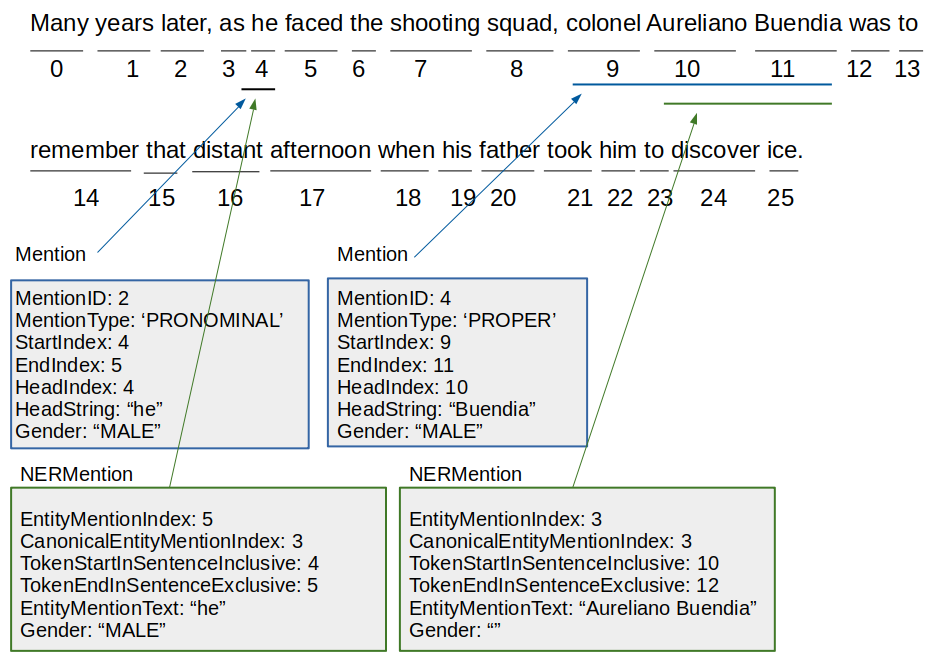
\includegraphics[scale=0.5]{solapamiento_esquema}
	\caption{Solapamiento entre menciones de correferencia (Mention) y de entidad (NERMention).}
	\label{fig:solapamiento_esquema}
\end{figure}

En base a estas observaciones se pueden determinar algunas reglas para decidir qué menciones se refieren a qué personaje. Como en el proceso de canonicalización explicado en la sección \ref{sec:nerextract_corenlp}, se considera que dos nombres coinciden cuando su distancia de edición \cite{levenshtein_1966} es menor que una distancia máxima, que se fija según lo largo que sea el nombre. Así, tenemos:

\begin{enumerate}
	\item Todas las NERMention que tengan el mismo \textit{canonicalEntityMentionIndex} se consideran como el mismo personaje, y el atributo \textit{entityMentionText} se considera el nombre del mismo.
	\item Identificar las Mention que también son menciones de entidad. Dichas Mention se consideran como el mismo personaje que el de la NERMention si sus nombres coninciden.
	\item De las Mention que hayan podido ser identificadas como pertenecientes a un personaje, obtener su cluster de correferencia y considerar a todas las Mention de dicho cluster como pertenecientes a dicho personaje, pero sólo si 1) El atributo \textit{gender} de ambas menciones son el mismo, y 2) El atributo \textit{headString} de ambas Mention coinciden.
\end{enumerate}

El resultado de este proceso es una lista de diccionarios de python que representa a cada personaje, conteniendo su nombre, su género, el número de veces que es mencionado, a qué clusters pertenece, etc.

Esta lista aún es bastante imperfecta. De entrada, los identificadores de entidad y de cluster asignados a cada mención dependen del \textit{Document}, y dada la estructura del programa, la mayoría de relatos van a tener asociados dos o más \textit{Document}, lo que significa que hay personajes con exactamente el mismo nombre y género que aparecen como dos personajes distintos, porque no comparten el mismo \textit{canonicalEntityMentionIndex} ni ningún cluster de correferencia. Además, esta forma de identificar personajes significa que si alguno tiene un apodo, o si a un personaje se le llama de forma consistente por su apellido en una zona del texto y por su nombre en otro, aparecerá como dos personajes distintos. Para mitigar estos errores, utilicé el proceso de canonicalización de personajes de la sección \ref{sec:nerextract_tagger}.
También vamos a aprovechar el proceso de canonicalización para determinar el género de un personaje de forma definitiva, y para ello vamos a aprovechar nuevamente que estamos manejando fanfics y que, por lo general, los autores etiquetan sus fanfics. No todos ellos etiquetan el género de sus personajes, pero algunos sí, ya que hay personas a las que le gusta explorar la personalidad o sexualidad de los personajes mediante técnicas como cambiarles el género o darles una expresión ambigua. Algunos ejemplos de las etiquetas que se suelen usar para indicar el género de un personaje son 'He/Him Pronouns for Crowley', 'Androgynous Crowley' o 'Female!Crowley'.

Teniendo en cuenta todos estos factores, la canonicalización de un personaje consiste en estos pasos:
\begin{enumerate}
	\item Identificar si es canon o no, utilizando los nombres de cada candidato y comparándolos con los nombres y apodos de los personajes canon, igual que en la sección \ref{sec:nerextract_tagger}.
	
	\item Identificar el género del personaje:
	\begin{enumerate}
		\item  Obtener las etiquetas su fanfic y comprobar si hay alguna etiqueta que indique el género del personaje. Si la hay, el personaje se considera de ese género.
		\item Si no hay ninguna etiqueta, nos quedamos con el género que CoreNLP le haya asignado.
		\item Si CoreNLP no le ha asignado ningún género ('UNKNOWN', o simplemente el \textit{string} vacío ''), le asignamos el género del personaje canon. Por tanto, si el personaje no es canon, su género seguirá siendo desconocido.
	\end{enumerate}
\end{enumerate}

Este proceso resuelve los problemas relacionados con tener los mismos personajes procesados en distintos \textit{Document}, y asegura que una mención será identificada con el personaje canon tanto si menciona el nombre, el apellido o sólo un apodo. Discrimina por género de tal manera que si se le asignan géneros distintos al mismo personaje, se cuentan las menciones de cada uno de modo que al final cada personaje tiene una cuenta de menciones masculinas, femeninas, neutras o desconocidas. De esta manera es más probable identificar correctamente a un personaje con su correspondiente en el canon aunque el género no concuerde.

Todos este proceso de extracción de personajes se lleva a cabo mediante una clase CoreNLPDataProcessor, que se encuentra encapsulada junto a CoreWrapper en un programa llamado \textit{corenlp\_util.py}. CoreNLPDataProcessor, además de extraer personajes, también tiene función de análisis de sentimiento, como se explicará en la sección \ref{sec:main}.

En la figura \ref{fig:ner_extraction_corenlp} hay un esquema que explica de forma visual todo este proceso de extracción de personajes.

\begin{figure}[!h]
	\centering
	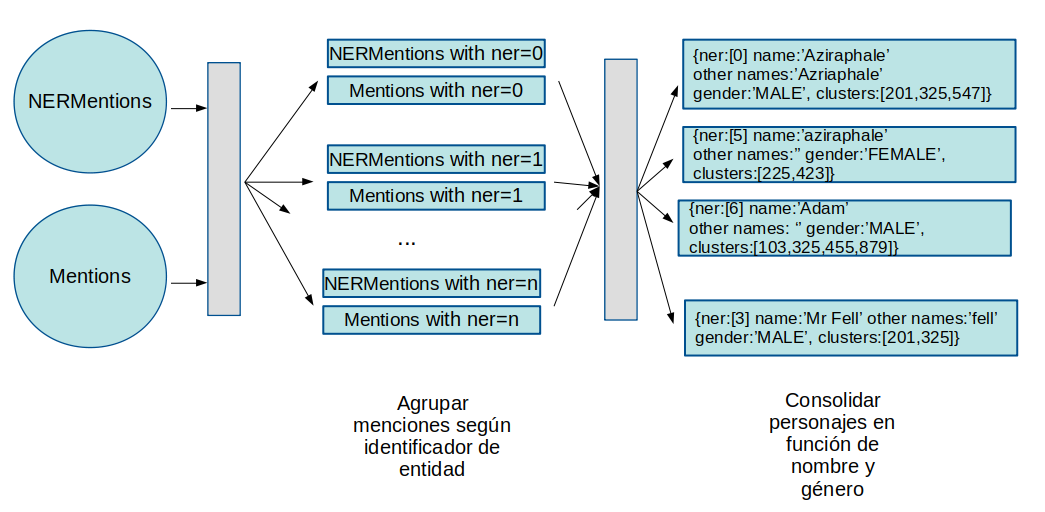
\includegraphics[scale=0.6]{core_ner_extraction}
	\caption{Esquema sobre el proceso de extracción de personajes con CoreNLP.}
	\label{fig:ner_extraction_corenlp}
\end{figure}


\subsection{Algoritmo de identificación de relaciones}

Las relaciones que definen un fanfic son las amistades, los enemigos y, principalmente, los amantes. Extraer relaciones a partir de texto natural es una tarea compleja de por sí, y tratar de detectar este tipo concreto de relaciones en literatura de género puede presentar un reto mayor, puesto que las relaciones sentimentales tienden a representarse de forma implícita, de modo que el lector aprende quiénes son amigos y quiénes enemigos a través de las acciones de los personajes. Además, la ambigüedad, la heterogeneidad y la experimentación son partes naturales de cualquier proceso creativo, por lo que un conjunto de obras no representará una misma relación de forma uniforme, incluso si es entre los mismos personajes.

Encontrar una estrategia para abordar este problema requiere exploración y creatividad, y ya que había empezado el proyecto con NLTK, me pareció natural comenzar la búsqueda por ahí.

El extractor de relaciones de NLTK funciona mediante reglas: después de extraer las entidades nombradas del texto, se puede utilizar el módulo \textit{relextract} para dividir el texto en listas de fragmentos del texto que contienen dichas entidades, y aplicar reglas basadas en expresiones regulares que definan la relación entre las entidades. La regla puede incluir etiquetas de rol morfológico en la expresión regular, y \textit{relextract} permite filtrar por etiqueta IOB, lo que le da algo más de flexibilidad.

Por ejemplo, para extraer una relación de lugar entre una organización y una localización, se puede crear una expresión regular que busque la palabra clave 'in' en el texto, e indicarle a \textit{relextract} que sólo te interesan los fragmentos de texto que tengan una entidad de tipo 'ORG' seguida de una entidad de tipo 'LOC':
\begin{lstlisting}[style=consola, caption=Ejemplo de código que utiliza el módulo \textit{regexp} de NLTK para extraer relaciones de lugar y mostrarlas por pantalla. Adaptado del capítulo 7 de Natural Language Processing with Python \cite{bird_2012}]
IN = re.compile(r'.*\bin\b(?!\b.+ing\b)')

for doc in parsed_docs:
	for rel in nltk.sem.extract_rels('ORG','LOC', doc, pattern=IN):
		print(nltk.sem.show_raw_rtuple(rel))

\end{lstlisting}

Existen proyectos que utilizan este módulo de NLTK para extraer relaciones como \textit{DateOfBirth} y \textit{HasParent}  \cite{jose_2017}, pero es evidente que es un método poco adecuado para el tipo de proyecto que estaba intentando hacer.

Estos programas basados en reglas dependen de localizar palabras claves en el texto, y aunque existen palabras clave para identificar relaciones sociales (\textit{"love"}, \textit{"kiss"}, \textit{"hug"}, \textit{"friend"}, \textit{"kill"}, \textit{"hate"}, etc), lo cierto es que la naturaleza de la expresión literaria hace que este método, incluso a simple vista, parezca bastante ingenuo. No sólo es perfectamente posible expresar amor, amistad y odio sin usar "palabras clave" asociadas con dichos sentimientos, sino que en un texto literario raramente se escribe explícitamente \textit{Romeo loved Juliette}, si no que es más normal encontrar estructuras como \textit{'I love you', said Romeo}. En una frase así, no se menciona explícitamente a Julieta, pero pero un lector humano sabe si se refiere a ella por el contexto de la escena. Pero un programa que únicamente se preocupa de las etiquetas IOB de una frase no será capaz de unir ese \textit{you} con Julieta (ni, ya puestos, el \textit{I} con Romeo).

Descartado el extractor de relaciones de NLTK, empiezo a buscar opciones en otras librerías. El Stanford Natural Language Processing Group publicó un extractor de relaciones como parte de las funciones de CoreNLP, pero las relaciones que está entrenado para detectar (\textit{Live\_In, Located\_In, OrgBased\_In, Work\_For, None}) no parecen útiles para el proyecto. Por tanto, entrenar mi propio modelo para relaciones sociales parece la única solución.

Crear un modelo de regresión logística con NLTK, similar al identificador de entidades, requería que el texto ya estuviera etiquetado con las relaciones. Los autores de AO3 usan etiquetas que es posible extraer las relaciones a partir del archivo HTML de cada fanfic, pero es una etiqueta a nivel del texto completo, no a nivel de frase, que es como trabaja NLTK. Dejando de lado NLTK por el momento, decidí explorar soluciones usando clustering y modelado de temas.

\subsubsection{Primeras estrategias: Clustering y LDA}
\label{sec:relextract}
Decidir si dos personajes son amigos, enemigos o amantes (sin tener ninguna información previa sobre la obra) puede requerir leer el texto completo, con lo cual es razonable utilizarlo para el análisis y asignar una etiqueta de 'romance', 'amistad' o 'enemistad' al texto en su conjunto, más que etiquetar ciertas palabras y personajes del mismo.

Por tanto, dado un conjunto de textos al azar, podría llegarse a la conclusión de cuáles contienen romance, cuáles amistad y cuáles enemistad observando si hay similitudes entre ellos. Con este enfoque, parece una tarea adecuada para un algoritmo de clustering.

Para comprobar cómo de útil sería esta estrategia utilicé el RFE dataset, cuya creación está explicada en la sección \ref{sec:limpiezadatos}. Esperaba que teniendo tres conjuntos claros en los que el tema era evidente sirviese para ver cómo de eficaz es el clustering para la tarea general, que sería poder decir si hay romance en un texto incluso si no es el tema central del mismo.


Una vez creados los conjuntos, utilicé la librería \textit{Scikit-Learn} en conjunto con NLTK para crear el programa de clustering. Para preprocesar el texto se utilizan los métodos de NLTK para \textit{tokenizar} y \textit{lemmatizar} los textos, además de crear un conjunto de \textit{stopwords}, palabras comunes en inglés pero que no aportan mucha información sobre el mismo (preposiciones, pronombres, puntuación, demostrativos, etc).
Después de preprocesar el texto se procede a extraer las características relevantes del mismo, para lo cual se utiliza el módulo \textit{TfidfVectorizer} de \textit{Scikit-Learn}. Su trabajo es 'vectorizar' el texto de manera que sus características principales queden expresadas en un formato que el algoritmo de clustering pueda entender, cosa que hace asignando un peso a cada palabra dependiendo del número de ocurrencias de la misma (esto se llama \textit{bag of words}). Hay vectorizadores que asignan más peso cuanta más frecuencia, pero esto hace que palabras muy comunes pero con poco valor informativo roben protagonismo a palabras menos frecuentes pero más interesantes. El vectorizador 'Tf-Idf' (\textit{Term frequency-Inverse document frequency}), en cambio, multiplica la frecuencia de una palabra en un documento por un componente \textit{idf} que, como se ve en la fórmula \ref{for:idf}, está basado en la frecuencia de ese término en todos los documentos. Los vectores resultantes se normalizan usando la norma de Euclides; más información está disponible en la guía de usuario de \textit{Scikit-Learn} \cite{sklearn_feature}. 

\begin{figure}
	\begin{equation}
	\text{idf}(t) = \log{\frac{1+n}{1+\text{df}(t)}}+1 
	\label{for:idf}
	\end{equation}
	\caption{Componente idf del vectorizador Tf-Idf. \textit
		{t} se refire al término cuyo peso está determinando, \textit{n} al número total de documentos y \textit{df} a la frecuencia de \textit{t} en este documento.}
	
\end{figure}

Con los textos ya preprocesados y convertidos en vectores \textit{tf-idf} se puede crear un modelo de clustering, en este caso utilizando el módulo \textit{KMeans} de \textit{Scikit-Learn}. KMeans es un algoritmo que crea clusters de tal forma que cada uno tenga la misma varianza, minimizando la suma de los cuadrados de las distancias entre los miembros de cada grupo (fórmula \ref{for:ineria}).

\begin{figure}[h]
	\begin{equation}
	\sum_{i=0}^{n}\min_{\mu_j \in C}{||x_i - \mu_j ||^2}
	\label{for:ineria}
	\end{equation}
	\caption{Criterio de la suma de cuadrados. \textit{n} es el total de textos, con \textit{x} perteneciendo a \textit{n}. \textit{C} es el número de clusters, con mu siendo la media de las muestras \textit{x} de cada cluster. El algoritmo KMeans reduce esta suma todo lo posible.}
	
\end{figure}

Además del código necesario para crear el modelo KMeans y procesar los daños, añadí código para evaluar el modelo e imprimir un diagrama de puntos con los clusters. Tras probar dos tokenizers distintos y varias combinaciones con los parámetros del vectorizador y el modelo, los resultados se pueden ver en la figura \ref{fig:kmeanresult}.

\begin{figure}[!h]
	\centering
	
	\begin{subfigure}{.4\textwidth}
		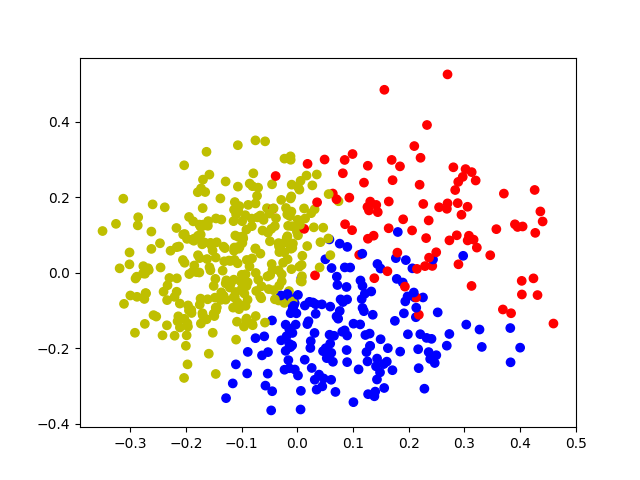
\includegraphics[scale=0.4]{kmeans_tokenizer2}
		\caption[aaaaa]{El código utilizado para crear este diagrama fue escrito por \href{https://stackoverflow.com/questions/57626286/how-to-plot-text-clusters}{Matt L en StackOverflow}\protect\footnotemark.}
	\end{subfigure}%
	\begin{subfigure}{.5\textwidth}
		\centering
		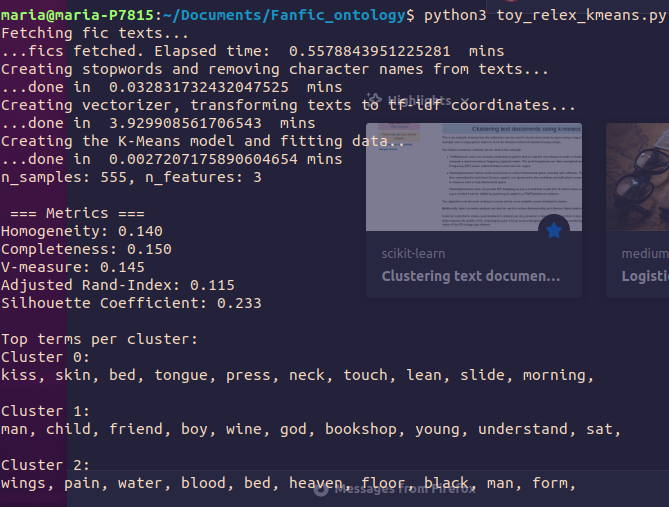
\includegraphics[scale=0.3]{ejecucion_kmeans_tokv2_0}
	\end{subfigure}
		
	\caption{A la derecha, ejecución de \textit{toy\_relex\_kmeans}, mostrando su evaluación. La homogeneidad se cumple cuando ningún cluster contiene miembros que pertenezcan a categorías distintas en los datos reales. La completitud se satisface si todos los miembros de una de las categorías reales pertenecen al mismo cluster. A la izquierda, el diagrama creado por el programa.}
	\label{fig:kmeanresult}
\end{figure}


\footnotetext{https://stackoverflow.com/questions/57626286/how-to-plot-text-clusters}

Los resultados no son muy buenos. Aunque los términos de cada cluster parecen prometedores, ninguna métrica sube del 0.1, lo que indica que las categorías del clustering son sólo un poco mejores que haberlas asignado al azar, y que hay mucho solapamiento entre clusters.

Puesto que para crear el modelo he utilizado datos filtrados a propósito para modelar cada categoría tan bien como fuera posible, con la esperanza de poder usarlo como posible semilla para un sistema más general, esto supone un gran problema.

Busqué entonces otra estrategia, utilizando un modelo de temas más que uno de clustering. El modelado de temas con el algoritmo LDA parece también una buena opción para este problema, puesto que al contrario que el clustering clásico, LDA asigna a cada documento una distribución de temas en cada uno. Esto se ajusta a este análisis, puesto que aunque he intentado crear \textit{datasets} 'perfectos' que traten un único tipo de relación en cada uno, lo cierto es que lo normal en un relato es que estén mezcladas.

LDA es un algoritmo que descubre temas de forma no supervisada. Trabaja bajo la asunción de que cada documento es un conjunto de temas, y que cada tema es un conjunto de palabras. Empieza asignando cada a palabra a un conjunto al azar de temas, y en cada iteración mejora la asignación. 

Al igual que en el programa anterior, LDA requiere un preprocesado del texto, con lo que utilizo los dos \textit{tokenizers} del algoritmo de clustering. \textit{Scikit-Learn} carece de modelo LDA, por lo que utilizo el de la librería \textit{gensim}. LDA también trata los textos como un \textit{bag of words}, pero no es necesario vectorizarlos antes de usarlos para entrenar el modelo, que devolverá  lista de palabras por tema, junto con la probabilidad de que esa palabra pertenezca a dicho tema.

Tras preprocesar los textos de forma similar a como se hizo con clustering y entrenar el modelo LDA, se observan los resultados en la figura \ref{fig:topicresult1}.

\begin{figure}
	\begin{subfigure}{\textwidth}
		\hspace{-1cm}
		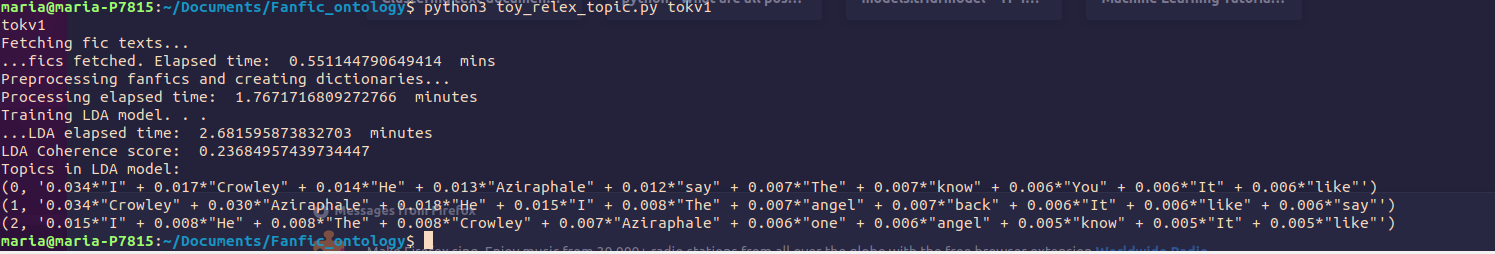
\includegraphics[scale=0.35]{ejecucion_topic_v1_0}
		\caption{Filtrado: sólo puntuación.}
		\label{fig:topicresult1}
	
	\end{subfigure}
	\begin{subfigure}{\textwidth}
		\hspace{-1cm}
		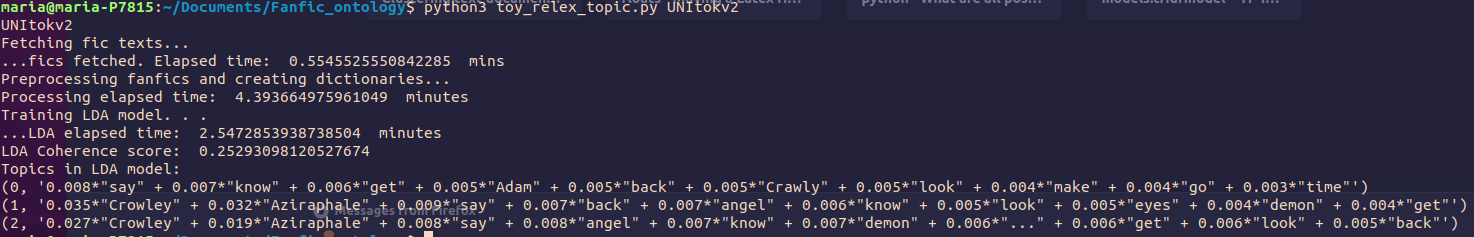
\includegraphics[scale=0.35]{ejecucion_topic_v2_0}
		\caption{Filtrado: puntuación, pronombres, determinantes, etc.}
		\label{fig:topicresult2}
	\end{subfigure}

	\caption{Ejecución de \textit{toy\_relex\_lda}, con distintos criterios de filtrado. Además se muestran los 10 términos más relevantes de cada tema, y su probabilidad de pertenecer a dicho tema.}

\end{figure}

Los resultados son un poco decepcionantes, pues ninguno de los 10 términos más relevantes por tema tiene siquiera un 0.1\% de probabilidad de pertenecer a su tema.
Tampoco es sorprende que no sean muy relevantes, pues aparecen muchos pronombres, determinantes e incluso algún número. Aprovechando el etiquetado de rol morfológico de NLTK, se retiran esas palabras y se crea un nuevo modelo, cuya ejecución está en la figura \ref{fig:topicresult2}.


Estos resultados, sin embargo, tampoco son muy convincentes. La puntuación de coherencia, que indica cómo de adecuado es el número de temas para los datos analizados, es 0.23 en el primer caso y 0.25 en el segundo. Es un resultado que se puede mejorar afinando los hiperparámetros de LDA, para lo cual se utiliza el programa \textit{topic\_evaluate.py}, que prueba diferentes valores para \textit{alpha} (densidad documento-tema) y \textit{beta} (densidad palabra-tema) del modelo LDA de \textit{gensim}. Los resultados de su ejecución se guardan en el archivo \textit{lda\_evaluation.csv}, y en la figura \ref{fig:lda_eval0} se puede ver que la puntuación de coherencia se puede mejorar bastante para tres temas con los hiperparámetros correctos, pero como evidencia la figura \ref{fig:lda_eval1}, queda muy lejos del 0.42 de coherencia que se puede conseguir si se permite subir el número de temas a nueve. No parece, por tanto, que este modelo sea el más adecuado para buscar las relaciones que se buscan.


\begin{figure}
	\centering
	\begin{subfigure}{\textwidth}
		%\hspace{-1cm}
		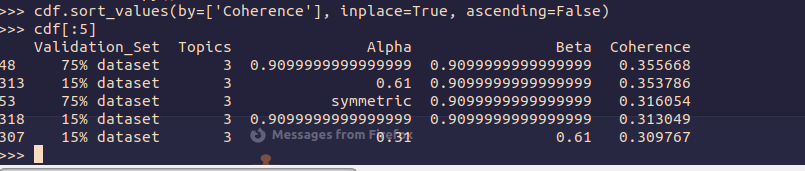
\includegraphics[scale=0.5]{lda_evaluate0}
		\caption{Mejores puntuaciones de coherencia para 3 temas.}
		\label{fig:lda_eval0}
		
	\end{subfigure}
	\begin{subfigure}{\textwidth}
		%\hspace{-1cm}
		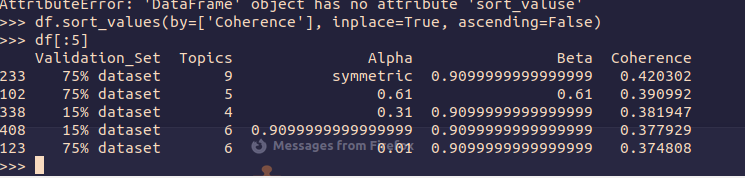
\includegraphics[scale=0.5]{lda_evaluate1}
		\caption{Parámetros con las mejores puntuaciones de coherencia de toda la prueba.}
		\label{fig:lda_eval1}
	\end{subfigure}
	
	\caption{Resultados de \textit{topic\_evaluate.py}, visualizados y ordenados con la ayuda de \textit{pandas}. Se pueden observar qué número de temas y qué hiperparámetros dan mejores puntuaciones de coherencia para el modelo LDA creado a partir del RFE dataset.}
	
\end{figure}



%\begin{itemize}
%	\item El modelo B tenía en cuenta sustantivos, adverbios y verbos.
%	\item El modelo C tenía en cuenta sustantivos, adjetivos y verbos.
%	\item El modelo D tenía en cuenta sustantivos, adverbios, adjetivos y verbos.
%\end{itemize}

%Además de utilizar distintas categorías morfológicas, también probé distintos tamaños para el set de entrenamiento, de modo que cada modelo tiene dos versiones: una entrenada con 5000 fanfics y otra entrenada con 10000.

%Para la evaluación de los modelos, simplemente los puse a clasificar textos nuevos, contando la cantidad de aciertos de cada uno y calculando el \textit{hit ratio} de cada uno. Los resultados aparecen en la primera tabla de la figura \ref{table:topic_evaluation}.

%\begin{gather*}
%hit\_ratio = %\frac{correct\_guesses}{total\_number\_of\_guesses}
%\end{gather*}

%\begin{figure}
%	\caption{Porcentaje de aciertos de cada modelo. Cada prueba se realizó tres veces.}
%	\label{table:topic_evaluation}
%	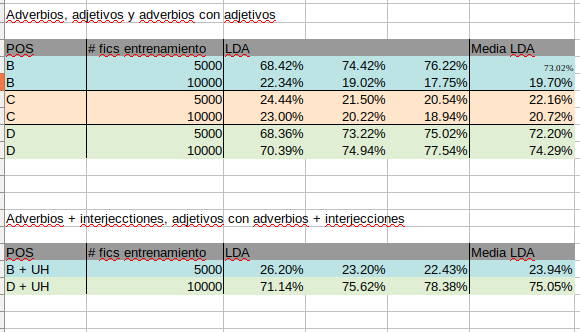
\includegraphics[scale=0.6]{topic_evaluate_table_v2}
%	\centering
%\end{figure}

%Las primeras pruebas mostraron que los modelos B y D eran los que arrojaban mejores resultados. Observando qué otras categorías morfológicas el \textit{tagger} de NLTK puede identificar, pensé que añadir interjecciones a los modelos podría aumentar su precisión. Llamé B+UH y D+UH a los modelos resultantes, y repetí las pruebas. Los resultados están en la segunda tabla de la figura \ref{table:topic_evaluation}.

%Curiosamente, el modelo D fue mejorado ligeramente teniendo en cuenta las interjecciones, pero el modelo B empeoró considerablemente.


\subsubsection{Correferencia con CoreNLP}
\label{sec:correferencia}
Tras varias pruebas con los algoritmos de clustering y LDA, encontré \textit{CorenNLP}, un servidor de Stanford NLP Group que realiza diversos tipos de extracción de información y análisis de lenguaje natural, entre ellos, resolución de correferencia.

Volviendo al ejemplo de Romeo y Julieta, una frase como \textit{'I love you', said Romeo}, extraída de un texto más largo en la que el contexto es que Romeo está hablando con Julieta, da poca información a un algoritmo que no es capaz de entender a qué personajes se refieren los pronombres \textit{I} y \textit{you}. Sin embargo, si se aplicase resolución de correferencia sobre el texto, a ojos del algoritmo la frase se convertiría en \textit{'Romeo love Juliette', said Romeo}, con lo que el algoritmo entiende mucho mejor qué está pasando en esta frase y a quiénes afecta.\label{nota:corref}

\textit{CoreNLP} da acceso a esa posibilidad. Aunque está programado en java, cuenta con un módulo de python llamado \textit{Stanza}, con lo que creé algunos programas para familiarizarme con su funcionamiento y la idea que quería desarrollar. El primero de estos programas, \textit{toy\_relex.py}, no hace más que buscar las frases que contengan el verbo 'to love' y al menos una entidad, elegida de antemano. El segundo programa, \textit{toy\_relex\_v2.py} expande este concepto usando \textit{CoreNLP}, utilizando tanto su función de identificación de entidades como la de solución de correferencia para obtener las 'cadenas de correferencia' del texto, utilizándolas para enlazar cada pronombre del texto con la entidad a la que se refiere. La idea sigue siendo seleccionar las frases que tengan el verbo \textit{'to love'}, pero en vez de quedarme únicamente con aquellas en las que se nombren explícitamente a un personaje, también me quedo con aquellas en las que los pronombres formen parte de una cadena de correferencia.

Para poder llevar a cabo todo esto, fue necesario estudiar con atención las propiedades de los objetos que utiliza \textit{Stanza}, que por suerte están bien \href{https://github.com/stanfordnlp/stanza/blob/master/doc/CoreNLP.proto}{documentadas}, y hacer muchas pruebas y visualización de datos, como se puede ver en las figuras \ref{fig:core_visualization_0} y \ref{fig:core_visualization_1}.


\begin{figure}
	\centering
	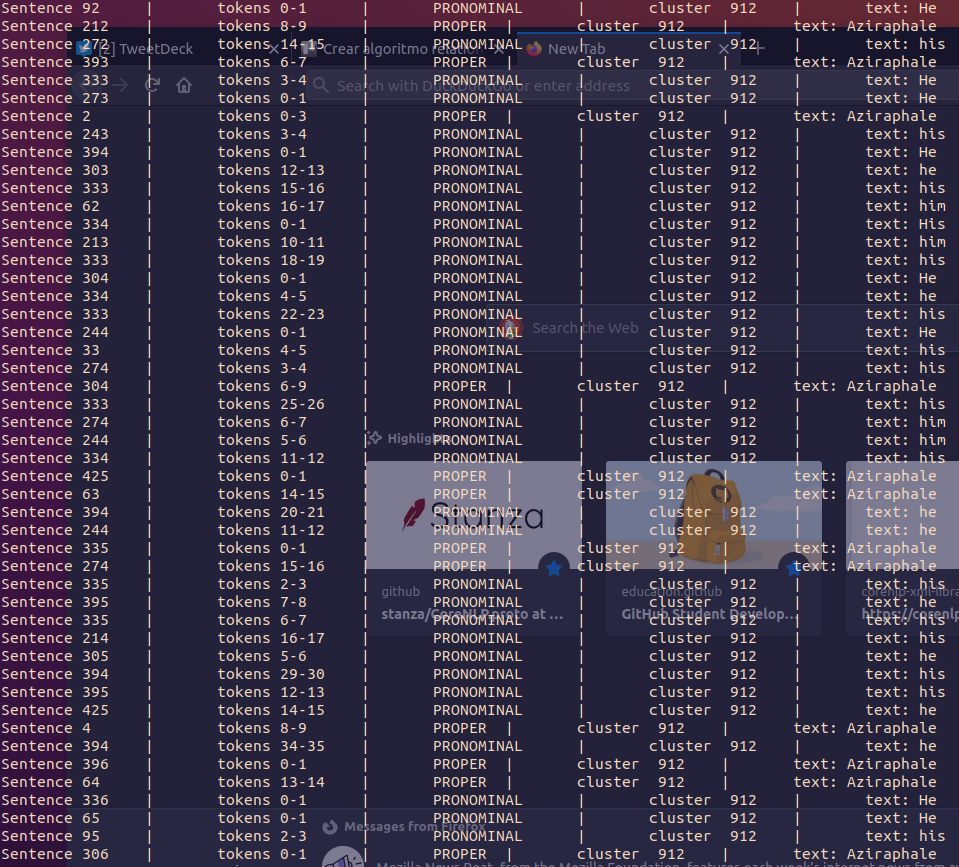
\includegraphics[scale=0.45]{core_vis_1}
	\caption{Visualización de la información proporcionada por \textit{CoreNLP}}
	\label{fig:core_visualization_0}
\end{figure}

\begin{figure}
	\centering
	\begin{subfigure}{.45\textwidth}
		\centering
		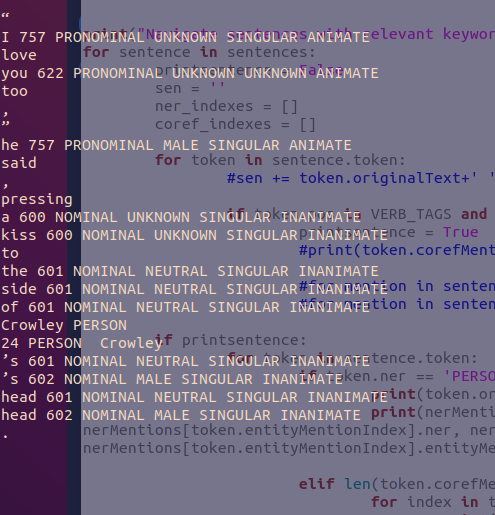
\includegraphics[scale=0.4]{core_vis_3}
	\end{subfigure}%
	\begin{subfigure}{.45\textwidth}
		\centering
		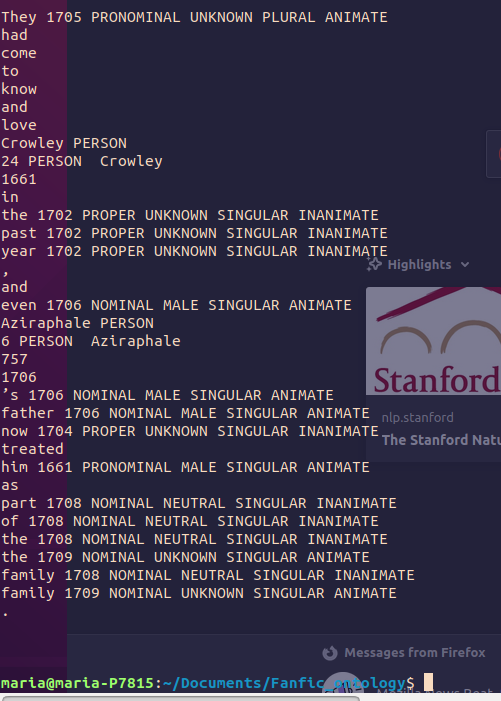
\includegraphics[scale=0.4]{core_vis_4}
	\end{subfigure}

	\caption{Visualización de frases particulares con anotaciones de correferencia de \textit{CoreNLP}}
	\label{fig:core_visualization_1}
\end{figure}

Tras analizar toda esta información, entender la indexación de los objetos de \textit{Stanza} y ganar experiencia manejándolos, se hizo evidente que el siguiente paso sería crear un programa cuya función fuese resumir la información proporcionada por CoreNLP de forma que sea útil para identificar relaciones entre personajes. En particular, mi intención era usarlo con el RFE dataset y tratar de identificar relaciones en él.
El problema era que el RFE dataset es bastante grande, y enseguida se hizo evidente que era necesario guardar la información proporcionada por CoreNLP en un archivo para no malgastar horas de trabajo. Ya que los objetos de \textit{Stanza} no tienen una forma sencilla de ser almacenados directamente, acabé creando un programa que, tras recoger las respuestas del servidor, resumía la información más relevante y la guardaba en dos archivos csv: 

\begin{itemize}
	\item fic\_characters.csv (tabla \ref{table:fic_characters}) almacena los personajes de cada fanfic, junto con su correspondiente en el canon y toda la información necesaria para identificar en qué frases de qué fanfic aparece (clusters, identificador, etc).
	\item fic\_sentences (tabla \ref{table:fic_sentences}) almacena los fanfics frase a frase, junto con los identificadores y clusters de los personajes mencionados en ellas. Decidí almacenar sólo las frases que mencionan personajes en vez de todas las del fanfic porque estaba orientando este archivo a la identificación de relaciones entre personajes, por lo que parecía razonable asumir que las frases con más información serían aquellas en las que se mencionan personajes.
\end{itemize}

%\missingfigure{fig:esquema indexacion Corenlp}

El desarrollo de este programa no fue trivial, debido a la complejidad de la indexación de \textit{Stanza} y otros problemas derivados de la naturaleza del proyecto, como por ejemplo, si un personaje aparece marcado como masculino en 20 menciones y femenino en 3, ¿Deberían considerarse personajes distintos? ¿Asumo que todas las menciones de un cluster se refieren a un único personaje, incluso si algunos nombres son radicalmente distintos del resto?
Para resolver todas estas preguntas y alcanzar un programa funcional fui pasando por varias etapas y distintos programas, que con el tiempo refinaría y acabaría encapsulando en \textit{corenlp\_util.py} para su uso posterior en el programa final. En esta parte del proyecto sin embargo utilicé los programas de \textit{corenlp\_wrapper.py} y \textit{ner\_and\_sen\_extraction\_v2.py}, que se pueden considerar versiones anteriores a las utilizadas en \text{corenlp\_util.py}, y por tanto muchos de los problemas mencionados en la sección \ref{sec:nerextract_corenlp} relacionados con la latencia y errores de servidor fueron resueltos durante su desarrollo. Además de estos problemas, hubo que limpiar y revisar el formato de cada \textit{string} y lista, ya que el archivo CSV estaba configurado para procesar cada punto y coma como un separador entre columnas, lo cual añadía columnas extra cada vez que encontraba un punto y coma en cualquier parte del texto.
 
\begin{table}[]
	\resizebox{\textwidth}{!}{%
	\begin{tabular}{lllllll}
		ficID & Dataset & senID & Sentiment & Verbs & nerIDs & Clusters         \\
		57    & ROMANCE & 2     & Positive  & Crowley flashed a grin over his shoulder .                                                                                       & 0      & 452              \\
		57    & ROMANCE & 5     & Positive  & He grabbed the long pole that served as a door handle and pulled it open .                                                       & 0      & 452, 18          \\
		57    & ROMANCE & 10    & Negative  & He cautiously side - stepped around an especially small one .                                                                    & 0      & 33, 452          \\
		57    & ROMANCE & 11    & Neutral   & “ They ’re not going to bite you , ” Crowley laughed . & 0      & 452, 36, 37, 113
	\end{tabular}%
}
	\caption{Estructura de \textit{fic\_sentences.csv}}
	\label{table:fic_sentences}
\end{table}
 
\begin{table}[]
	\resizebox{\textwidth}{!}{%
		\begin{tabular}{lllllll}
			ficID & nerID & Name & Gender & Mentions & clusterID & canonID         \\
			57    & 0     & ng    & UNKNOWN & 193 & 279, 452, 116, 251, 435, 448, 517, 545      & -1       \\
			57    & 15, 80, 95 & aziraphale & MALE & 54  & 279                                  & 4         \\
			57    & 146, 151 & crowley  & MALE & 23  & 452                                      & 8          \\
			70    & 0     & crowley  & NEUTRAL & 9   & 1                                        & 8
		\end{tabular}%
	}
	\caption{Estructura de \textit{fic\_characters.csv}}
	\label{table:fic_characters}
\end{table}

Una vez procesado todo el RFE dataset y completados los CSV, utilicé la información almacenada ellos para realizar varias técnicas de análisis de texto natural, con la esperanza de hallar algún patrón, bigrama o palabra significativa que me ayudara a identificar relaciones entre personajes.

En primer lugar quise buscar si había algún verbo que fuera característico de cada dataset, por lo que extraje y lematicé los verbos de cada frase usando las herramientas de NLTK. En la primera pasada los verbos más repetidos en todos los dataset fueron verbos muy comunes en inglés, como 'say', 'go', 'get', 'make', 'look', etc. de modo que para eliminar ruido hice otro análisis eliminándolos. Para hacer más fácil la comparación y a modo de ejemplo, se muestra la distribución de frecuencias de los verbos en el dataset de romance en la figura \ref{fig:r_verbs}-\ref{fig:r_verbs_removed}.


\begin{figure}[h!]
	\centering
	\begin{subfigure}{\textwidth}
		%\hspace{-1cm}
		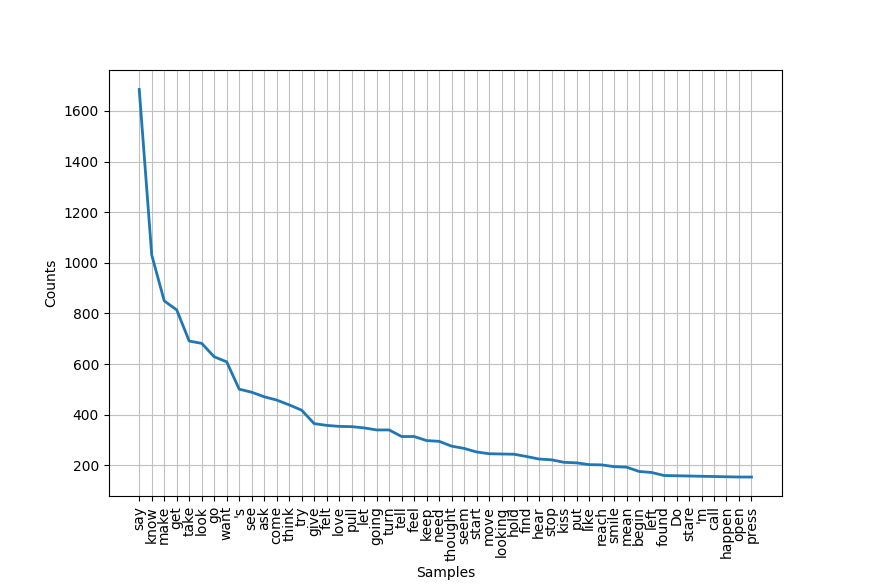
\includegraphics[scale=0.7]{r_verbs_0}
		\caption{Verbos más frecuentes en el dataset de romance.}
		\label{fig:r_verbs}
		
	\end{subfigure}
	\begin{subfigure}{\textwidth}
		%\hspace{-1cm}
		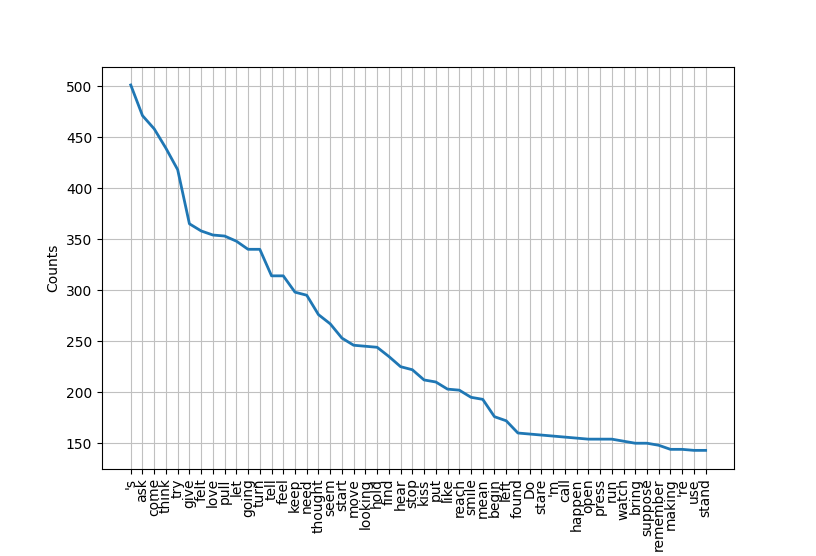
\includegraphics[scale=0.7]{r_verbs_1}
		\caption{Verbos más frecuentes en el dataset de romance, tras retirar los más comunes.}
		\label{fig:r_verbs_removed}
	\end{subfigure}
	
	%\caption{...}
	
\end{figure}

\begin{comment}
\begin{figure}[h!]
	\centering
	\begin{subfigure}{\textwidth}
		%\hspace{-1cm}
		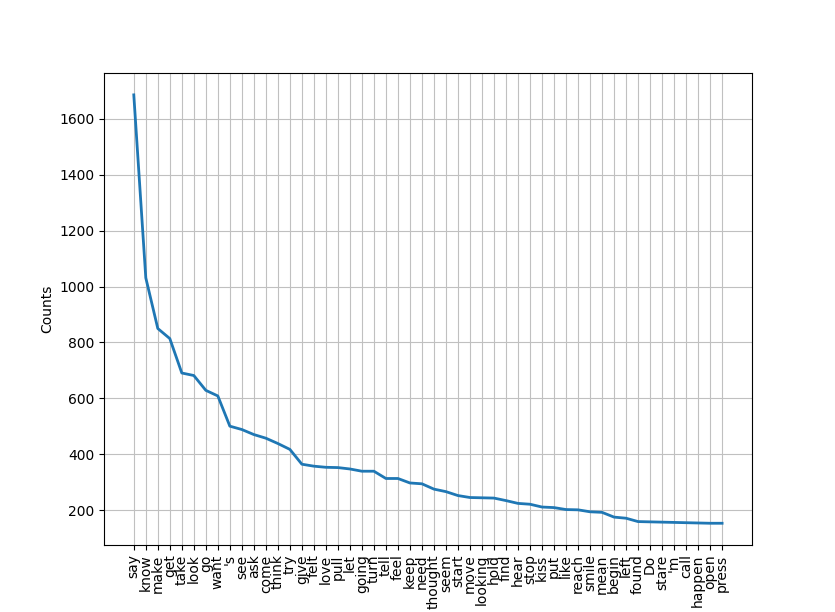
\includegraphics[scale=0.7]{f_verbs_0}
		\caption{Verbos más frecuentes en el dataset de amistad.}
		\label{fig:f_verb_freq_in_dataset}
		
	\end{subfigure}
	\begin{subfigure}{\textwidth}
		%\hspace{-1cm}
		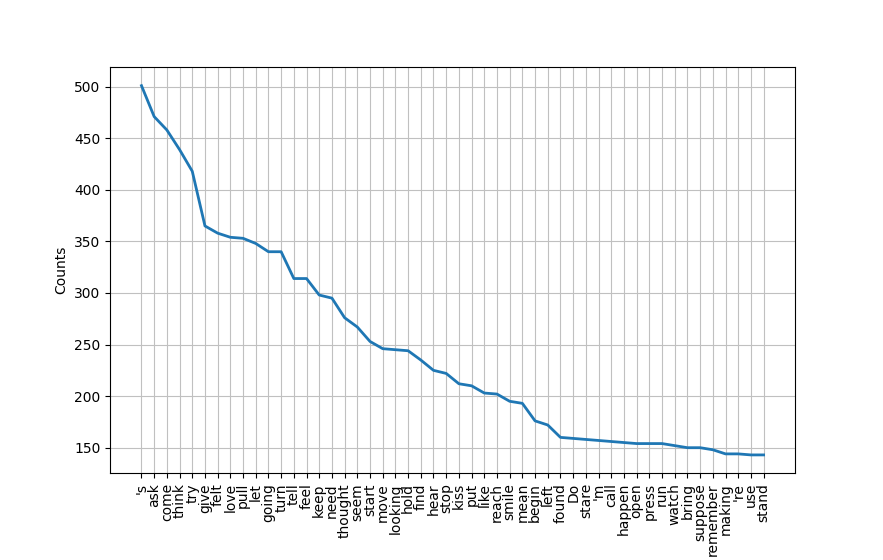
\includegraphics[scale=0.7]{f_verbs_1}
		\caption{Verbos más frecuentes en el dataset de amistad, tras retirar los más comunes.}
		\label{fig:f_verb_freq_removed}
	\end{subfigure}
	
	%\caption{...}
	
\end{figure}


\begin{figure}[!h]
	\centering
	\begin{subfigure}{\textwidth}
		%\hspace{-1cm}
		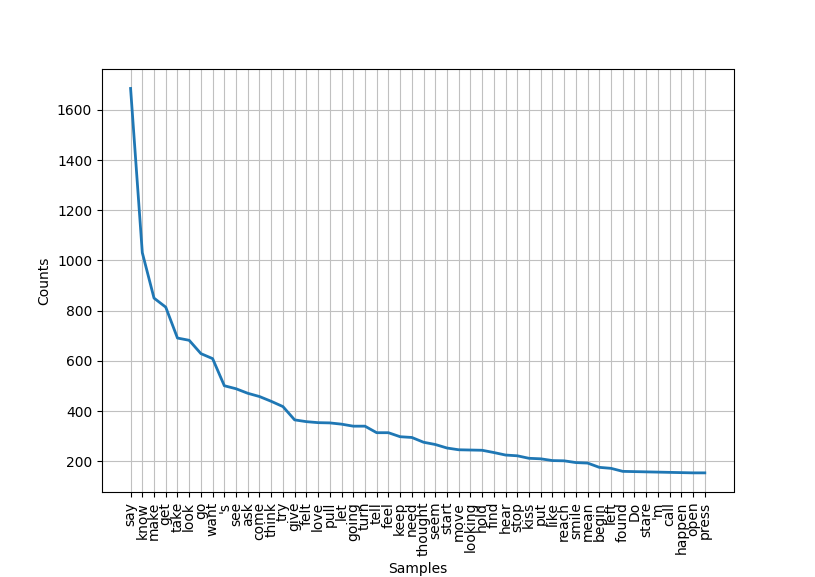
\includegraphics[scale=0.7]{e_verbs_0}
		\caption{Verbos más frecuentes en el dataset de enemistad.}
		\label{fig:e_verb_freq_in_dataset}
		
	\end{subfigure}
	\begin{subfigure}{\textwidth}
		%\hspace{-1cm}
		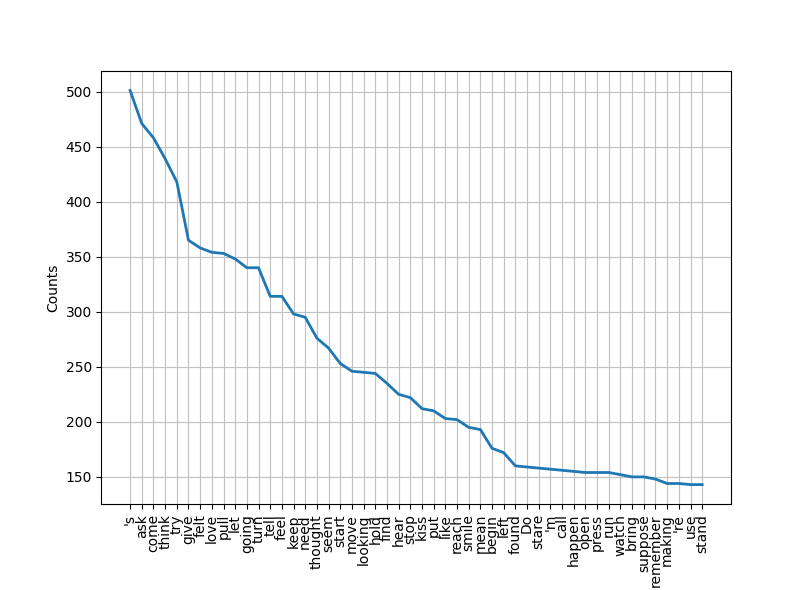
\includegraphics[scale=0.7]{e_verbs_1}
		\caption{Verbos más frecuentes en el dataset de enemistad, tras retirar los más comunes.}
		\label{fig:e_verb_freq_removed}
	\end{subfigure}
	
	%\caption{...}
	
\end{figure}

\end{comment}

Desafortunadamente, ni siquiera eliminar los verbos más frecuentes parecía dar un resultado claramente distintivo para cada dataset, por lo que decidí utilizar NLTK para buscar bigramas y trigramas característicos (figuras \ref{fig:r_btrigram_lik}-\ref{fig:e_btrigram_lik}). Pero tampoco parece haber un alguna combinación distintiva aquí, los n-gramas siguen siendo bastante parecidos de un dataset a otro y utilizan casi las mismas palabras.

\begin{comment}
\begin{figure}
	\centering
	\begin{subfigure}{\textwidth}
		%\hspace{-1cm}
		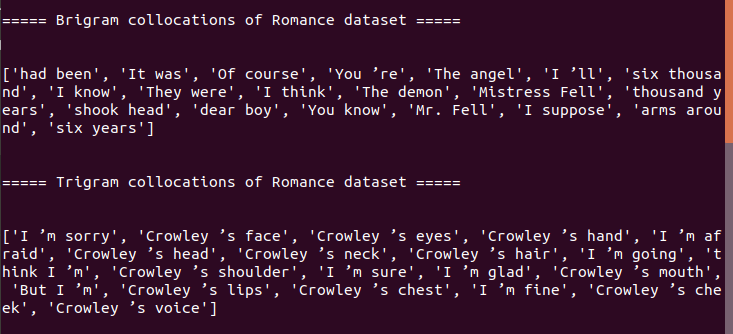
\includegraphics[scale=0.5]{r_btrigrams_lik}
		\caption{Bigramas y trigramas con mayor likelihood en el dataset de romance}
	%	\label{fig:r_btrigram_lik}
		
	\end{subfigure}
	\begin{subfigure}{\textwidth}
		%\hspace{-1cm}
		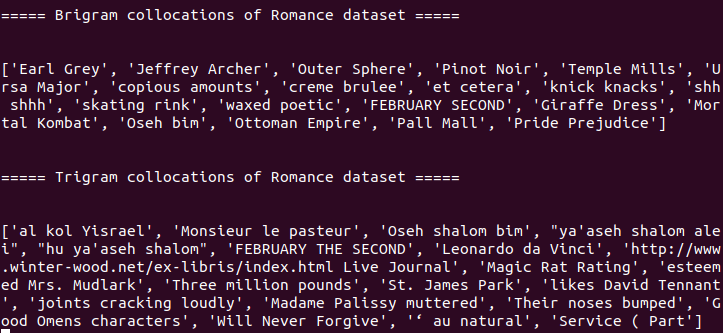
\includegraphics[scale=0.5]{r_btrigrams_pmi}
		\caption{Bigramas y trigramas con mayor pmi en el dataset de romance}
		\label{fig:r_btrigram_pmi}
	\end{subfigure}
	
	%\caption{...}
	
\end{figure}

\begin{figure}
	\centering
	\begin{subfigure}{\textwidth}
		%\hspace{-1cm}
		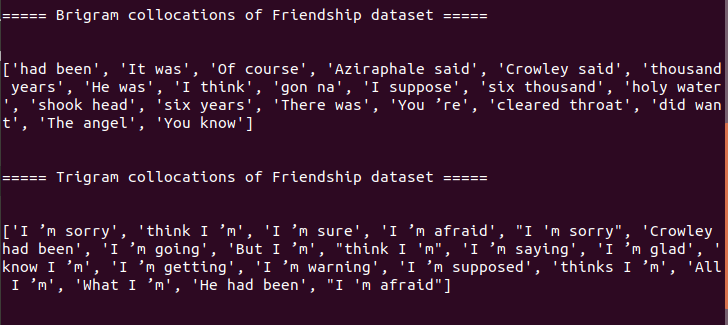
\includegraphics[scale=0.5]{f_btrigrams_lik}
		\caption{Bigramas y trigramas con mayor likelihood en el dataset de amistad}
	%	\label{fig:f_btrigram_lik}
		
	\end{subfigure}
	\begin{subfigure}{\textwidth}
		%\hspace{-1cm}
		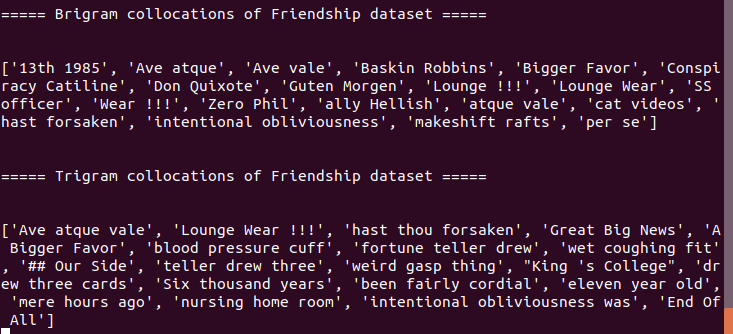
\includegraphics[scale=0.5]{f_btrigrams_pmi}
		\caption{Bigramas y trigramas con mayor pmi en el dataset de amistad}
		\label{fig:f_btrigram_pmi}
	\end{subfigure}
	
	%\caption{...}
	
\end{figure}

\begin{figure}
	\centering
	\begin{subfigure}{\textwidth}
		%\hspace{-1cm}
		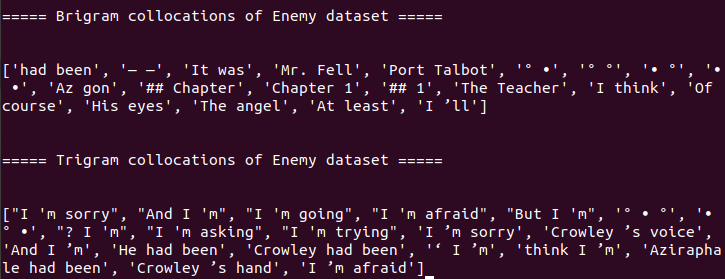
\includegraphics[scale=0.5]{e_btrigrams_lik}
		\caption{Bigramas y trigramas con mayor likelihood en el dataset de enemistad}
		%\label{fig:e_btrigram_lik}
		
	\end{subfigure}
	\begin{subfigure}{\textwidth}
		%\hspace{-1cm}
		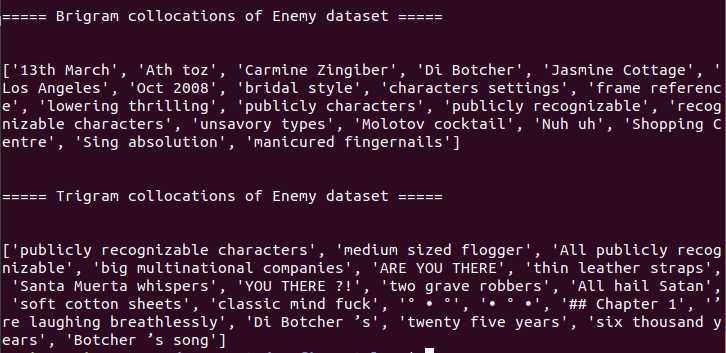
\includegraphics[scale=0.5]{e_btrigrams_pmi}
		\caption{Bigramas y trigramas con mayor pmi en el dataset de enemistad}
		\label{fig:e_btrigram_pmi}
	\end{subfigure}

\end{figure}

\end{comment}


\begin{figure}[t!]
	\centering
	
	\begin{subfigure}{\textwidth}
		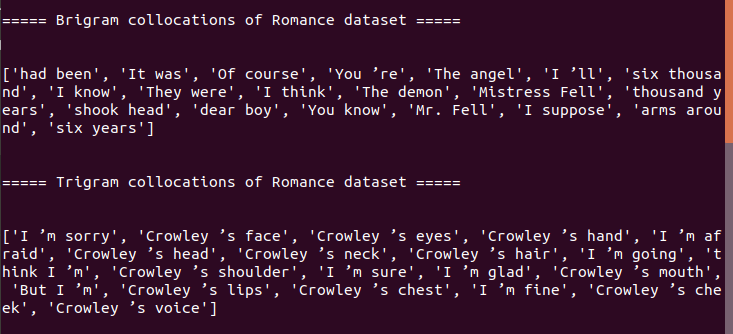
\includegraphics[scale=0.65]{r_btrigrams_lik}
		\caption{Bigramas y trigramas con mayor likelihood en el dataset de romance.}
		\label{fig:r_btrigram_lik}
	\end{subfigure}

	\begin{subfigure}{\textwidth}
		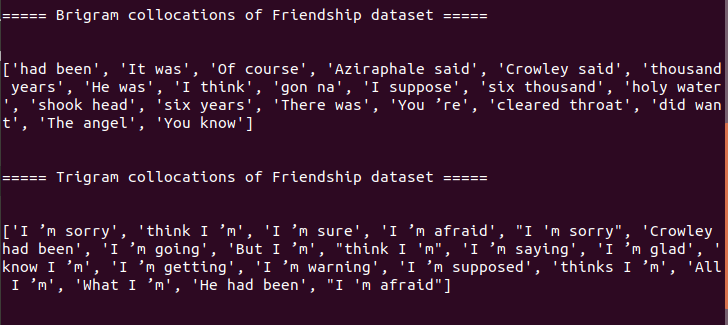
\includegraphics[scale=0.65]{f_btrigrams_lik}
		\caption{Bigramas y trigramas con mayor likelihood en el dataset de amistad.}
		\label{fig:f_btrigram_lik}
	\end{subfigure}

	\begin{subfigure}{\textwidth}
		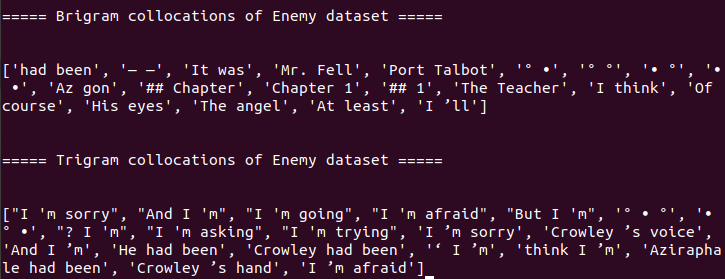
\includegraphics[scale=0.65]{e_btrigrams_lik}
		\caption{Bigramas y trigramas con mayor likelihood en el dataset de enemistad.}
		\label{fig:e_btrigram_lik}
	\end{subfigure}
\end{figure}

En un último intento de buscar algún patrón, decidí volver extraer la distrución de frecuencia de verbos, bigramas y trigramas, pero esta vez utilizando únicamente las frases en las que se mencione a dos personajes en concreto, en vez de todas las frases del relato. Estos personajes son elegidos de antemano, utilizando los identificadores propocionados por CoreNLP (tal y como se ve en la tabla \ref{table:fic_sentences}).

 La distribución de frecuencias se puede ver en la figura \ref{fig:r_verb_freq_in_character_mentions}.
 
 Sobra decir que los resultados tampoco fueron muy prometedores. Por tanto dejo para un trabajo la parte de extracción de relaciones, y el resto del proyecto se centra en la extracción de personajes nombrados y determinación de su género.

\begin{figure}
	\centering
	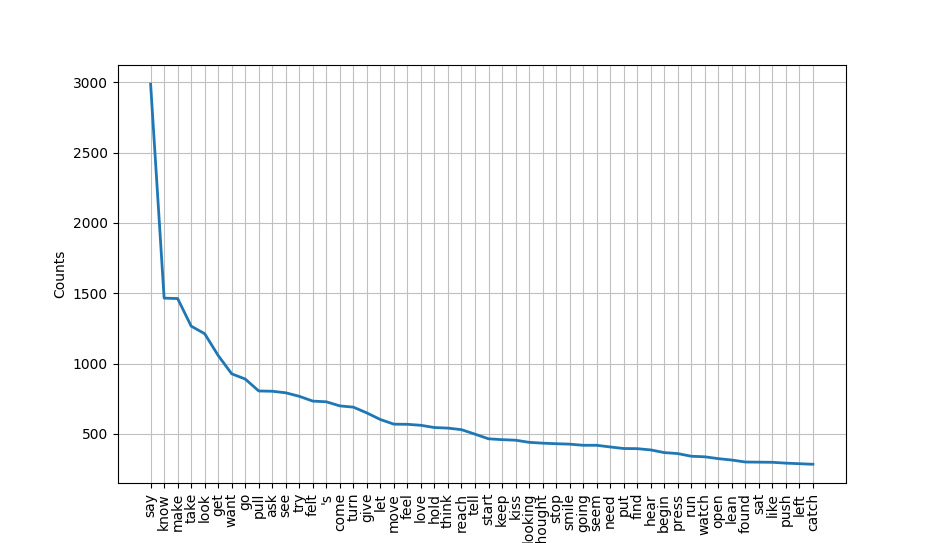
\includegraphics[scale=0.6]{ac_rverbs_2}
	\caption{Verbos más frecuentes en el dataset de romance en las frases que mencionan a dos personajes concretos.}
	\label{fig:r_verb_freq_in_character_mentions}
\end{figure}


\begin{comment}

\begin{figure}
	\centering
	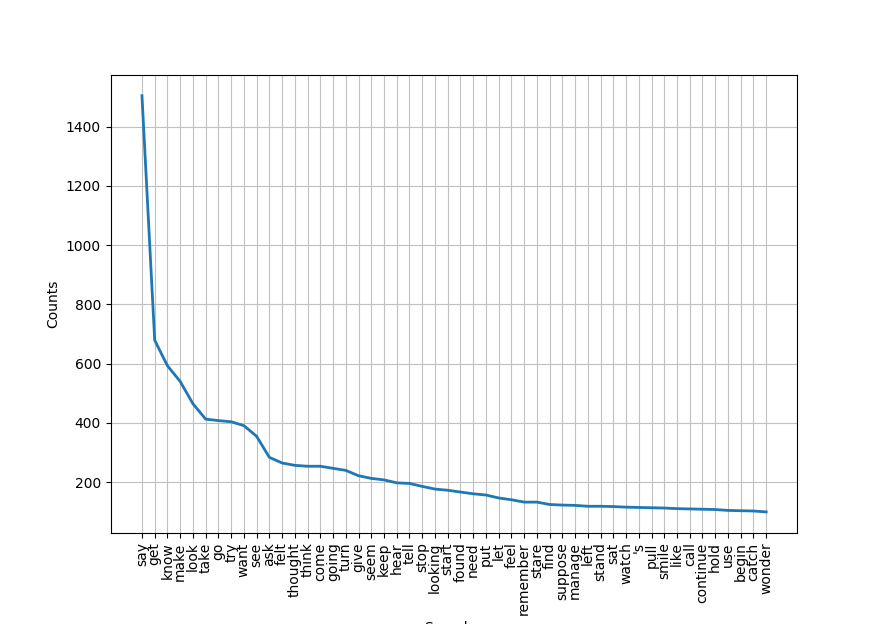
\includegraphics[scale=0.6]{ac_fverbs_2}
	\caption{Verbos más frecuentes en el dataset de amsitad en las frases que mencionan a dos personajes concretos.}
	\label{fig:f_verb_freq_in_character_mentions}
\end{figure}


\begin{figure}
	\centering
	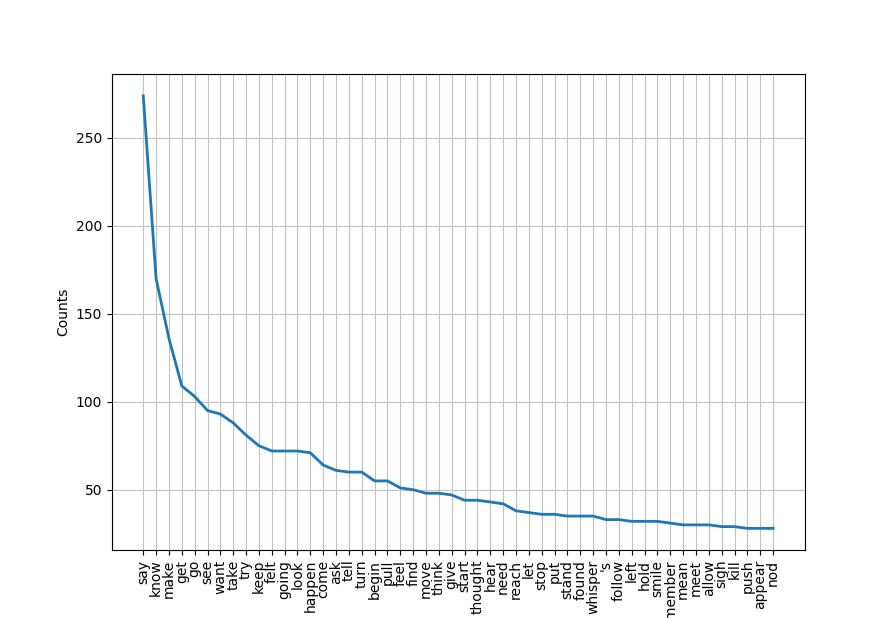
\includegraphics[scale=0.6]{crowhas_everbs_0}
	\caption{Verbos más frecuentes en el dataset de enemistad en las frases que mencionan a dos personajes concretos.}
	\label{fig:e_verb_freq_in_character_mentions}
\end{figure}

\end{comment}



\cleardoublepage
\section{PROGRAMA PRINCIPAL: fic\_character\_extractor }
\label{sec:main}

El programa principal se lanza desde la terminal y tiene dos posibles comandos:
\begin{itemize}
	\item \textit{\finalProgramName <fic\_index>}, que analizará el fanfic cuyo identificador sea \textit{fic\_index}. Por tanto, se comprueba que el usuario no introduzca un identificador menor que 0 ni mayor que 20190.
	\item \textit{\finalProgramName}, que analizará un fanfic elegido al azar del total de fanfics disponibles. Debido a la latencia de CoreNLP, evita elegir un fanfic que tenga más de 50000 caracteres.
\end{itemize}

En ambos casos el programa utiliza la clase FanficGetter del módulo \textit{fanfic\_util} para extraer el fanfic elegido, obteniendo así el objeto Fanfic que encapsula toda la información necesaria del mismo. A continuación, se siguen los siguientes pasos:

\begin{enumerate}
	\item Identificación de entidades con NERTagger: El texto del fanfic es \textit{tokenizado} en frases y palabras antes de etiquetar cada palabra con su rol morfológico, usando para ello las herramientas de procesado de texto de NLTK. A continuación, se utiliza la función \textit{parse()} de la clase NERTagger del módulo \textit{NER\_tagger}(\ref{sec:nerextract_tagger}) para extraer los personajes del texto.
	\item Identificación de entidades con CoreNLP: se utiliza la clase CoreWrapper para enviar el texto al servidor de CoreNLP, y la clase CoreNLPDataProcessor extrae los personajes a partir de la respuesta. Ambas clases pertenecen al módulo \textit{corenlp\_util}(\ref{sec:nerextract_corenlp}).
	\item Análisis de sentimiento con CoreNLP: se utiliza la clase CoreNLPDataProcessor de \textit{corenlp\_util} para extraer el sentimiento del fanfic y mostrar si es principalmente positivo o negativo.
	\item Mostrar en pantalla los resultados, junto con el título y etiquetas de personaje del fanfic.
\end{enumerate}

Las etiquetas de personaje de un fanfic son simplemente la forma del autor de indicar qué personajes aparecen en él. Por motivos técnicos evidentes, los autores se limitan a etiquetar a los personajes más importantes del texto, por lo que es esperable que NERTagger y CoreNLP encuentren más personajes en el texto. Sin embargo, como mínimo no deberían dejar sin identificar ninguno de los personajes etiquetados.
Las etiquetas de personaje, como el título, son metadatos del fanfic que se extraen directamente del mismo usando la clase FanficHTMLHandler del módulo \textit{fanfic\_util}.

Los personajes detectados por NERTagger y CoreNLP serán algo distintos, pero por lo general las coincidencias son bastante consistentes. Las menciones de los personajes de NERTagger siempre serán más bajas que los de CoreNLP, ya que éste último no sólo cuenta cuando al personaje se le menciona por el nombre, sino que también puede detectar menciones puramente pronominales.

Las menciones de CoreNLP aparecerán fraccionadas según género, de modo que un personaje puede tener 100 menciones masculinas, 3 femeninas, 0 neutras y 12 desconocidas (cuando no ha sido posible asignar ningún género a dicha mención). La intención de mostrar estos datos así es poder cuantificar cómo de seguro está el programa sobre el género de un personaje.



\cleardoublepage
\section{EVALUACIÓN DEL SISTEMA}
\label{sec:evaluacion}

Vamos a evaluar el programa según la cantidad de personajes correctamente identificados y si su género concuerda con el género que el personaje realmente tiene en el texto. Los motivos que me llevaron a elegir cada fanfic para cada prueba serán explicados en la misma, aunque todos tienen en común que no son demasiado largos, lo cual ayuda tanto a que yo como CoreNLP no tardemos mucho en obtener la información que necesitamos de ellos.

La mayoría de información aparece transcrita en tablas vez de ser pantallazos del programa, para ahorrar espacio, pero la información aparece en pantalla con el mismo formato.

\subsection{Prueba 1: Funciones básicas del programa con un texto largo (Fanfic 9)}
Escogí este fanfic para la primera prueba porque tiene muchos personajes, algunos de los cuales sólo se les menciona una o dos veces, y con 8821 palabras es un texto medianamente largo, útil para recabar información sobre los personajes. Además, este fic particular tiene varias erratas, lo que también pondrá a prueba la capacidad del programa para identificar un personaje con el nombre ligeramente incorrecto.

Ejecutar el comando \textit{\finalProgramName 9}. En la figura \ref{fig:eval1_metadata} se muestran los metadatos del fanfic, y en las tablas \ref{table:eval1_nertagger} y \ref{table:eval1_nercorenlp} se han transcrito los personajes identificados por NERTagger y CoreNLPDataProcessor.

\begin{figure}[h]
	\centering
	\label{fig:eval1_metadata}
	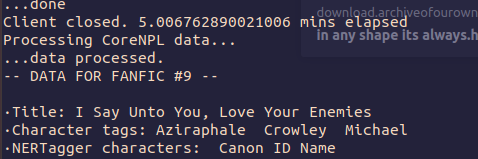
\includegraphics[scale=0.7]{eval1_metadata}
	\caption{Título y etiquetas de personaje del fanfic 9.}
\end{figure}

\begin{table}[t]
	\resizebox{\width}{0.8\height}{%
	\begin{tabular}{lll}
		Canon ID & Name            & Mentions         \\
		NO       & Lord Beezlebub  & 2       \\
		NO       & Lilith          & 1         \\
		14       & Did Gabriel     & 1          \\
		NO       & Ashmedai        & 11    \\
		4       & Aziraphale        & 42    \\
		NO       & Laradiri        & 16   \\
		NO       & Every Woman        & 1    \\
		NO       & Marut        & 1    \\
		NO       & Joe        & 1    \\
		NO       & Amides        & 1    \\
		NO       & Dr Dudders        & 1    \\
		NO       & History       & 1   \\
		14       & Gabriel        & 1    \\
		NO       & Butter        & 1    \\
		NO       & Alisha        & 1    \\
		4       & Aziraphale never        & 1    \\
		NO       & Mrs Beeton        & 1    \\
		NO       & Richard        & 1          \\
		NO       & Heavenly       & 1       \\
		4       & Azriaphale       & 1         \\
		4       & Mr Fell        & 2         \\
		NO       & Seamus Blackley        & 1        \\
		24       & Michael       & 1         \\
		NO       & Do NOT        & 1     \\
		10       & Death        & 1     \\
		14       & Sir Yes Sir Gabriel Sir       & 1        \\
		13       & Heaven        & 1     \\
		NO       & Ashemedai        & 1     \\
		9       & Dagon       & 1     \\
		NO       & Pride        & 1     \\
		8       & Crowley        & 45     \\
		NO       & So Below        & 1     \\
		NO       & Any       & 1     \\
		NO       & Inside        & 1     \\
		15       & God        & 1     \\
		NO       & Got        & 1     \\
		5       & Beezlebub       & 1     \\
		NO       & Word        & 1     \\
		8       & Mr Crowley        & 1     \\
		4       & Aziraphale        & 42     \\
		8       & Crowley One        & 1     \\
		15       & God Herself        & 1     \\
		NO       & Mr Solomons        & 3     \\
		NO       & Cookery Reformed        & 1     \\
		
	\end{tabular}%
}
\caption{Resultados de la ejecución de \finalProgramName para analizar fanfic 9}
\label{table:eval1_nertagger}
\end{table}

\begin{table}
	\resizebox{\textwidth}{!}{%
		\begin{tabular}{lllllll}
			Canon ID & Name            & MALE & FEMALE & NEUTRAL & UNKNOWN & Other names       \\
			1       & Agnes Nutter  & 0    &  1     &    0     &  0        & Agares \\
			4       & Aziraphale          & 147    & 0     & 4        & 0    &  aziraphale, Azriaphale, Fell, azirphale, azriaphale, consume Aziraphale, Azirphale     \\
			5      & Beelzebub     & 4     &  0    &  3       &0     & Beezlebub     \\
			8       & Crowley        & 104     &  0    &7         &0     & crawley, crowley, Shop  Crowley, Crawley      \\
			14       & Gabriel        & 6     &  0    &  0       &0     &   \\
			21       & Ligur        & 1    &    0  &   0      &    0 &       \\
			24       & Michael        & 2    & 0     &   0      & 0    &       \\
			25       & Newton Pulsifer        & 0    & 1     &         &     & Beeton      \\
			36       & Uriel        & 1    &    0  & 0        &0     &       \\
			NO       & Bentley        & 1    &  0    &  0       &   1  &       \\
			NO       & Somolons        & 3    &    0  & 0        &  0   &       \\
			NO       & Laradiri       & 0    &  0    & 0        &  1   &       \\
			NO       & Eden        & 0     & 0     &  0       & 1    &       \\
			NO       & Petronius        & 1     &  0    &0         &  0   &       \\
			NO       & Ashmedai        & 0     &   0   & 0        &1     &       \\
			NO       & Angelo        & 1    &     0 &0         & 0    &       \\
			NO       & Ashemedai        & 0     &0      &  0       & 4    &       \\
			NO       & Laradiri        &0   &   0   & 0        &1     &       \\
			NO       & Angelo        & 1     &  0    &    0     &    0 &       \\
			NO       & Richard       & 1     &   0   &   0      &  0   &       \\
			NO       & Ashmedai       & 0     &   0   &   0      &  3   &       \\
			NO       & Jane Austen       & 0     &   0   &   0      &  1   &       \\
			NO       & Richards       & 1     &   0   &   0      &  0   &       \\
			NO       & Marut       & 1     &   0   &   0      &  0   &       \\
			NO       & Joe       & 5     &   0   &   0      &  0   &       \\
			NO       & Laradiri       & 1     &   0   &   0      &  0   &       \\
			NO       & Alisha       & 0     &   2   &   0      &  0   &       \\
			NO       & Solomons       & 1     &   0   &   0      &  0   &       \\
			NO       & Perkins       & 1     &   0   &   0      &  0   &       \\
			NO       & Hannah Glasse       & 0     &   1   &   0      &  0   &       \\
			NO       & Jane Austen       & 0     &   1   &   0      &  0  &       \\
			NO       & Seamus Blackley       & 1    &   0   &   0      &  0   &       \\
			NO       & Jane Austen       & 0     &   2   &   0      &  0   &       \\
			NO       & Laradiri       & 0     &   0   &   0      &  42   &       \\
			NO       & Ashmedai       & 0     &   0   &   0      &  13   &       \\
			NO       & Ashmedai       & 0     &   0   &   0      &  2  &       \\
		\end{tabular}%
	}
	\caption{Resultados de la ejecución de \finalProgramName para analizar fanfic 9}
	\label{table:eval1_nercorenlp}
\end{table}

De entrada, tenemos los personajes de las etiquetas: Aziraphale, Crowley y Michael. Son los personajes que el autor decidió etiquetar, probablemente por considerarlos los más importantes, y los tres son identificados correctamente tanto por NERTagger como por CoreNLPDataProcessor.

NERTagger ha identificado 35 personajes distintos, de los cuales 8 identifica como canon. Sus resultados, mostrados en la tabla \ref{table:eval1_nertagger}, permite observar que lista en entradas distintas a personajes que son claramente el mismo pero con una errata (Ashemedai y Ashmedai, Azriaphale y Aziraphale), pero los identifica correctamente con el mismo personaje (Azriaphale y Aziraphale tienen ambos el identificador 4). Destacan las entradas 'Lord Beezlebub' y 'Beezlebub': ambas tienen la misma errata, pero el primero no aparece identificado como personaje canon, mientras que el segundo sí. Esto problamente sea por la distancia de edición y el tamaño de los nombres: 'Lord Beezlebub' son dos palabras y la más corta es Lord, con sólo 4 letras. Esto significa que el algoritmo explicado en la sección \ref{sec:nerextract_tagger} sobre cuándo coinciden dos nombres habrá considerado que la distancia máxima de edición sólo puede ser 1. Cuando hay dos palabras en un nombre, como en este caso, se escoge la que tenga la distancia de edición más pequeña, que en este caso sería la distancia entre 'Beezlebub' y 'Beelzebub',  que es 2, excediendo el límite de distancia. Sin embargo, cuando la única palabra en el nombre es 'Beezlebub' y se compara directamete con 'Beelzebub', al ser un nombre más largo la distancia máxima de edición es 3, y NERTagger por tanto lo identifica correctamente como canon.

También hay algunos personajes con nombres 'raros' como 'Did Gabriel' o 'Aziraphale never', en los que claramente NERTagger ha incluído en el nombre del personaje una palabra que no correspondía. Sin embargo, puesto que al menos parte del 'nombre' concide con un personaje canon, son identificados correctamente.

Los 8 personajes que identifica como canon están correctamente identificados excepto 'Heaven', que confunde un personaje canon llamado 'Raven'. En el texto aparecen otros tres personajes canon que el programa no ha detectado, y sólo dos personajes no canon (mencionados cada uno sólo una vez).

CoreNLPDataProcessor por su parte identifica 9 personajes canon, incluyendo a Ligur, que se le escapó a NERTagger. En la tabla \ref{table:eval1_nercorenlp} también podemos ver a los personajes Agnes Nutter y Newton Pulsifer, que en realidad no aparecenen el texto pero aparecen incorrectamente identificados como la versión canon de Agares y Beeton (de nuevo, debido a la distancia de edición). Todo el resto de personajes listados en la tabla son personajes reales que aparecen en el texto, y sus géneros están correctamente asignados en todos los casos excepto Beelzebub, que en esta historia tiene pronombres femeninos. También hay que destacar el personaje Laradiri, inventado por el autor y cuyo género no es definido en ningún momento, siendo referido únicamente con el pronombre neutro inglés \textit{they}. Como consecuencia, sus menciones aparecen maracadas como neutras o 'desconocidas'.

Sólo hay un personaje canon y un personaje no canon que ninguno de los dos programas han detectado.

Otro problema claro es que CoreNLPDataProcessor no parece capaz de consolidar correctamente los personajes que no son canon, apareciendo repetidos en vez de en una única entrada que recoja todas las menciones.


\subsection{Prueba 2: Género distinto del canon (Fanfic 2856)}
En este fanfic, el autor decidió cambiar el género de los protagonistas, por lo que en su historia los personajes Crowley y Aziraphale son dos mujeres. Es un relato con más de 3000 palabras, por lo que no debería de ser poca información.

Cambiar el género de personajes es bastante común en el género fanfic, y es éste uno de los motivos por los cuales analizar fanfiction puede ser tan interesante: los autores juegan con los personajes y exploran su psique desde muchos ángulos, incluído el de género. Nuestro programa debería identificar que, en este texto, la mayoría de menciones a Crowley y Aziraphale son femeninas.

\begin{figure}[h]
	\centering
	\label{fig:eval2_metadata}
	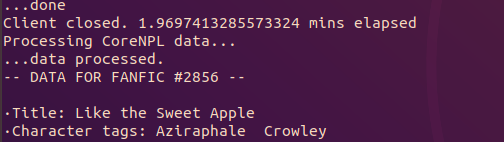
\includegraphics[scale=0.7]{eval2_metadata}
	\caption{Título y etiquetas de personaje del fanfic 2856.}
\end{figure}

\begin{table}[h]
	%\resizebox{\textwidth}{!}{%
	\begin{tabular}{lll}
		Canon ID & Name            & Mentions         \\
		NO       & Mesopotamia  & 1       \\
		NO       & How    & 1        \\
		NO       & Green     & 3          \\
		NO       & out       & 1    \\
		NO       & Eisheth      & 3    \\
		4       & Aziraphale      & 48   \\
		NO       & Unhand     & 1    \\
		38       & Azi  Eisheth       & 1   \\
		NO       & Always      & 1    \\
		8       & Crowley    & 62    \\
		NO       & See     & 1    \\
		NO       & No      & 1    \\
		4       & Rather     & 3    \\
		NO       & gorgeous   & 1    \\
		NO       & Just   & 1    \\
		NO       & Villain   & 1    \\
		NO       & Oh   & 4    \\
		NO       & Shouldn   & 1    \\
	\end{tabular}%
	%}
	\caption{Resultados de la ejecución de \finalProgramName para analizar fanfic 2856}
	\label{table:eval2_nertagger}
\end{table}

\begin{table}[h]
	\resizebox{\textwidth}{!}{%
		\begin{tabular}{lllllll}
			Canon ID & Name            & MALE & FEMALE & NEUTRAL & UNKNOWN & Other names       \\
			0      & Adam Young & 1   &   0    &  0       &    0      &  Adam \\
			4       & Aziraphale          & 217    &   0   & 1
			&0     &    \\
			8       & Crowley  & 445    &   0    &4
			& 0         & Crowley  Zadkiel \\
			NO       & Eisheth     & 0     & 0     & 0        & 2    &     \\
			NO       & Serpent of Eden     & 0     & 0   & 0        & 1    &     \\
			
		\end{tabular}%
	}
	\caption{Resultados de la ejecución de \finalProgramName para analizar fanfic 2856}
	\label{table:eval2_nercorenlp}
\end{table}

En la tabla \ref{table:eval2_nercorenlp} podemos ver que la detección de género ha fallado totalmente. A pesar de que no son referidos jamás en masculino en todo el texto, CoreNLPDataProcessor sigue asignándoles menciones masculinas de forma casi exclusiva.

Por lo demás, las identificaciones no son incorrectas. Como se puden comprobar con los metadatos de la figura \ref{fig:eval2_metadata}, Crowley y Aziraphale son correctamente identificados en el texto por ambos programas. En la tabla \ref{table:eval2_nertagger} se muestra que además de los dos protagonistas ha identificado otros 16 nombres, pero sólo 'Eisheth' es realmente otro personaje en el texto ('Mesopotamia' aparece, pero es obviamente un lugar). También confunde 'Rather' con un personaje canon, Aziraphale (Canon ID = 4), probablemente porque uno de sus apodos es \textit{'Brother} Francis', e inexplicablemente, confunde 'Azi Eisheth' con el personaje canon con ID = 38, cuyo nombre es 'Jeremey Wendsleydale' y que no se le menciona por ninguna parte en el texto.

CoreNLPDataProcessor, a pesar del fracaso con el género, identifica correctamente a Aziraphale, Crowley y Adam como personajes canon, e incluso que Crowley en este relato adopta el nombre 'Zadkiel' brevemente. También identifica a Eisheth y a 'Serpent of Eden', que en principio tendría que haber sido vinculado con Crowley, al ser 'Serpent' uno de sus apodos. No añade ningún personaje que no aparezca en el texto.

\begin{comment}

\subsection{Prueba 3: Etiquetas de género (Fanfic 9064)}
Puesto que parece difícil detectar el género utilizando puramente las capacidades de CoreNLPDataProcessor, vamos a buscar un fanfic que tenga una etiqueta indicando el género del personaje para ver si la parte que aprovecha los metadatos del fanfic a la hora de dilucidar el género de un personaje funciona correctamente. Para ello he elegido los fanfics 

%\begin{figure}
%	\centering
%	\includegraphics[scale=1]{imagefile}
%	\label{fig:eval3_metadata}
%	\caption{Título y etiquetas de personaje del fanfic 9064.}
%\end{figure}

\begin{table}
	%\resizebox{\textwidth}{!}{%
		\begin{tabular}{lll}
			Canon ID & Name            & Mentions         \\
			NO       & Lord Beezlebub  & 2       \\
			NO       & Lilith          & 1         \\
			14       & Did Gabriel     & 1          \\
			NO       & Ashmedai        & 11    \\
			4       & Aziraphale        & 42    \\
			NO       & Laradiri        & 16   \\
			NO       & Every Woman        & 1    \\
			NO       & Marut        & 1    \\
			NO       & Joe        & 1    \\
			NO       & Amides        & 1    \\
			NO       & Mr Dudders        & 1    \\
			NO       & History       & 1   \\
			14       & Gabriel        & 1    \\
			NO       & Butter        & 1    \\
			NO       & Alisha        & 1    \\
			4       & Aziraphale never        & 1    \\
			NO       & Mrs Beeton        & 1    \\
		\end{tabular}%
	%}
	\caption{Resultados de la ejecución de \finalProgramName para analizar fanfic 9}
	\label{table:eval3_nertagger}
\end{table}

\begin{table}
	\resizebox{\textwidth}{!}{%
		\begin{tabular}{lllllll}
			Canon ID & Name            & MALE & FEMALE & NEUTRAL & UNKNOWN & Other names       \\
			NO       & Lord Beezlebub  & 2    &       &         &          &  \\
			NO       & Lilith          & 1    &      &         &     &      \\
			14       & Did Gabriel     & 1     &      &         &     &      \\
			NO       & Ashmedai        & 11     &      &         &     &       \\
			4       & Aziraphale        & 42     &      &         &     &   \\
			NO       & Laradiri        & 16    &      &         &     &       \\
			NO       & Every Woman        & 1    &      &         &     &       \\
			NO       & Marut        & 1    &      &         &     &       \\
			NO       & Joe        & 1    &      &         &     &       \\
			NO       & Amides        & 1    &      &         &     &       \\
			NO       & Mr Dudders        & 1    &      &         &     &       \\
			NO       & History       & 1    &      &         &     &       \\
			14       & Gabriel        & 1     &      &         &     &       \\
			NO       & Butter        & 1     &      &         &     &       \\
			NO       & Alisha        & 1     &      &         &     &       \\
			4       & Aziraphale never        & 1    &      &         &     &       \\
			NO       & Mrs Beeton        & 1     &      &         &     &       \\
		\end{tabular}%
	}
	\caption{Resultados de la ejecución de \finalProgramName para analizar fanfic 9}
	\label{table:eval3_nercorenlp}
\end{table}

\end{comment}

\subsection{Prueba 3: Personajes que no son nombrados (Fanfic 2163)}
Decidí probar este fanfic porque los protagonistas Crowley y Azirphale aparecen, pero son vistos desde la perspectiva de dos extrañas que no les conocen, y por tanto, no saben sus nombres. Además, este fanfic tiene tan sólo 876 palabras, con lo que a la falta de nombres se le añade una información limitada.

Ejecutamos el comando \textit{\finalProgramName  2163}:

\begin{figure}[h]
	\centering
	\label{fig:eval4_metadata}
	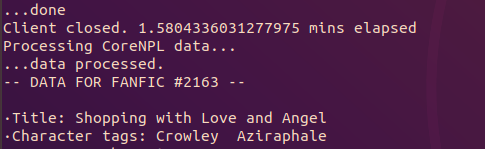
\includegraphics[scale=0.7]{eval4_metadata}
	\caption{Título y etiquetas de personaje del fanfic 2163.}
\end{figure}

\begin{table}[h]
	%\resizebox{\textwidth}{!}{%
	\begin{tabular}{lll}
		Canon ID & Name            & Mentions         \\
		NO       & Really inaccurate  & 1       \\
		NO       & Love       & 1        \\
		4       & Angel     & 8          \\
		NO       & Yeah        & 1    \\
		4       & Well       & 1    \\
		NO       & sort      & 1   \\
		NO       & Did      & 1    \\
		NO       & Oh       & 3    \\
		NO       & Really      & 1    \\
		NO       & Pardon     & 1    \\
		NO       & Olivia      & 7    \\
		NO       & Hey      & 1    \\
		NO       & Lauren      & 3    \\
		NO       & Um     & 1    \\
	\end{tabular}%
	%}
	\caption{Resultados de la ejecución de \finalProgramName para analizar fanfic 2163}
	\label{table:eval4_nertagger}
\end{table}

\begin{table}[h]
	\resizebox{\textwidth}{!}{%
		\begin{tabular}{lllllll}
			Canon ID & Name            & MALE & FEMALE & NEUTRAL & UNKNOWN & Other names       \\
			4       & Aziraphale          & 7    &   0   & 0
			&0     &    Angel  \\
			NO       & Angel Olivia  & 3    &   0    &0
			& 0         & \\
			NO       & Olivia     & 0     & 7     & 0        & 0    &     \\
			NO       & Lauren     & 0     & 4    & 0        & 0    &     \\
			NO       & Olivia    & 0     & 1     & 0        & 0    &     \\
			NO       & Olivia     & 0     & 1     & 0        & 0    &     \\
			NO       & Angel Olivia     & 0     & 0    & 0        & 24    &     \\
			NO       & Angel Olivia     & 0     & 6     & 0        & 0    &     \\
			
		\end{tabular}%
	}
	\caption{Resultados de la ejecución de \finalProgramName para analizar fanfic 2163}
	\label{table:eval4_nercorenlp}
\end{table}

Ambos programas han identificado correctamente a Lauren y Olivia, los personajes originales del autor desde cuya perspectiva se cuenta este relato. Ambas son también correctamente identificadas como personajes que no son canon (Canon ID es 'NO'), y en \ref{table:eval4_nercorenlp} podemos ver que todas sus menciones son femeninas excepto las de una de las entradas repetidas de 'Angel Olivia', que tiene 24 menciones 'desconocidas'.
Como en la prueba 2, tanto Crowley como Aziraphale son mujeres en esta historia, pero todas las menciones de Aziraphale son identificadas como masculinas. La buena noticia es que tanto NERTagger como CoreNLPDataProcessor han sido capaces de identificar correctamente a Aziraphale por su apodo 'angel', y, curiosamente, en la tabla \ref{table:eval4_nertagger} se puede ver que NERTagger también ha identificado que 'Love' en este relato es un apodo cariñoso para un personaje. Sin embargo, también identifica incorrectamente la palabra 'Well' como refiriéndose a Aziraphale (probablemente por parecido con uno de sus apodos, 'Fell').
Esto significa que NERTagger ha identificado 11 personajes, de los cuáles sólo 4 son correctos (aunque un humano puede detectar fácilmente qué nombres son los falsos positivos), mientras que CoreNLPDataProcessor ha identificado 4 personajes distintos, de los cuales dos son correctos y uno está correctamente identificado con su correspondiente canon, pero el género es incorrecto. 

Como se puede ver en los metadatos de la figura \ref{fig:eval4_metadata}, ambos programas han identificado correctamente a Aziraphale pero ninguno a Crowley; no es de extrañar, ya que ni su nombre ni ninguno de sus apodos es mencionado en todo el texto, y al propio Azirpahale sólo se le ha identificado por su apodo 'angel'. Sin embargo, NERTagger encuentra el nombre 'Love' y sabe que es un nombre; simplemente no tenía forma de saber que se refería a Crowley. CoreNLPDataProcessor no ha sido capaz de identificar 'Love' como un nombre.


\cleardoublepage

\section{CONCLUSIONES}


En este trabajo se ha desarrollado un sistema de extracción y análisis de textos de internet, utilizando técnicas de \textit{scraping} y procesado de texto natural.

En primer lugar se ha creado un corpus de relatos pertenecientes al género fanfiction a partir de los textos alojados en la web \href{https://www.archiveofourown.org/}{Archive of our Own}, y se ha utilizado este corpus para realizar pruebas, entrenamientos y experimentos que ayudaron en el desarrollo de un sistema de procesado de texto natural. Se han seleccionado textos en inglés que se basaran en el libro \textit{Good Omens} (Neil Gaiman y Terry Pratchett, 1990) y que tuvieran una cantidad mínima de palabras para asegurar que la obra estaba compuesta principalmente por texto (en vez de imágenes o audio), y se ha desarrollado un sistema de scrapers capaces de extraer los relatos de la web que tuvieran esas características. El resultado ha sido un corpus compuesto por archivos HTML para cuyo acceso y manejo se han desarrollado diversos objetos y funciones en python, encapsuladas en un módulo que he llamado \textit{fanfic\_util}. Además, aprovechando los metadatos de los relatos del corpus se han creado tres datasets, cada uno consistente en relatos de un sólo capítulo centrados en romance, amistad y enemistad, respectivamente. Estos datasets se utilizan para experimetnos durante la búsqueda de estrategias para la identificación de relaciones.

En el procesado de texto natural se han creado dos algoritmos de identificación de entidades, uno basado en naïve Bayes y otro en un modelo de regresión logística. Ambos fueron desarrollados con la librería NLTK de python (en conjunto con el módulo \textit{megam} en el caso del modelo de regresión logística), y entrenados con el corpus \textit{Groninger Meaning Bank}, que fue creado expresamente para entrenar algoritmos para identificar entidades en textos en inglés. La versión con el modelo de regresión logística consiguió mejores resultados, como se puede ver en la figura \ref{fig:ner_evaluation}, con lo que se decide utilizar esta versión bajo el nombre \textit{NER\_tagger}.

Para la parte de extracción de relaciones del procesado de texto natural, se han explorado varias estrategias. Usando \textit{sci-kit learn} y \textit{gensim} se han creado algoritmos de clustering y un modelo LDA, con la esperanza de que fueran capaces de clasificar correctamente a qué dataset pertenecía cada relato (romance, amistad o enemistad). La idea era que si podían clasificarlos correctamente, las características más relevantes de cada cluster o del modelo podrían utilizarse para refinar el algoritmo y crear una versión que pudiese identificar romance, amistad o enemistad incluso en textos largos donde no fueran el tema central, pero lamentablemente no se obtuvieron resultados mucho mejores que el azar.

La última estrategia para identificar relaciones consistía en explotar la correferencia pronominal en frases donde se nombraran a los personajes, utilizando para ello el servidor de Stanford CoreNLP mediante su biblioteca para python, \textit{Stanza}. La idea era identificar todas las menciones de un personaje en un texto, incluso aquellas que sólo se les mencionaran por el pronombre (\textit{he, she, they}), aumentando por tanto la cantidad de frases relevantes para el algoritmo. CoreNLP tiene, entre otras funciones, la capacidad de resolver esta correferencia pronominal en textos, por lo que se ha creado un conjunto de funciones para enviar peticiones de forma sencilla y controlada a su servidor, sin inundarlo, y manejar errores de red de forma que se pierda la menor de cantidad posible. Todas estas funciones han sido encapsuladas en un módulo que he llamado \textit{corenlp\_util}. Mediante este módulo los relatos de los datasets de romance, amistad y enemistad han sido procesados y etiquetados, y los resultados se han guardado en un archivo con el que se realizaron aún más experimentos para buscar alguna forma de identificar relaciones entre entidades. Estos últimos experimentos consistieron en buscar patrones relacionados con los verbos, adjetivos, bigramas o trigramas más frecuentes en las frases que mencionasen al menos a dos personajes, pero tampoco se pudo encontrar ningún patrón que fuese más relevante que el azar.

Decidí entonces dejar el desarrollo de un algoritmo de identificación de relaciones sociales entre personajes para el futuro, y me centré en el algoritmo de identificación de personajes. Ya tenía uno, basado en regresión logística, pero como durante el desarrollo de las pruebas con CoreNLP para realizar correferencia también tuve que manejar las funciones de CoreNLP para identificación de entidades, esto resultó en un segundo algoritmo de identificación de personajes que he llamado \textit{CoreNLPDataProcessor}, encapsulado también dentro del módulo \textit{corenlp\_util}. A diferencia de la versión basada en un modelo de regresión logística, esta versión puede identificar no sólo el nombre sino también el género del personaje, además de aprovechar la resolución de correferencia para identificar más menciones.

El resultado final por tanto, ha sido un programa que he llamado \textit{fic\_character extractor}, que utiliza ambos algoritmos de identificación de personajes para extraer información de un texto. Este programa ofrece al usuario la posibilidad de extraer personajes de cualquiera de los relatos del corpus creado en la primera parte del proyecto, dando la posibilidad de analizar uno al azar o introducir el identificador numérico de un relato particular. Entonces, el programa utiliza tanto \textit{NER\_tagger} como \textit{CoreNLPDataProcessor} para analizar el texto y mostrar al usuario el nombre de los personajes, si son canon o no, el número de menciones y, en el caso de este último, su género.

 De los objetivos originales expuestos en la introducción (\ref{sec:intro}), se han logrado con éxito cuatro de los seis objetivos, uno que ha fallado y el último, que se ha logrado en parte:
\begin{enumerate}
	\item Se ha conseguido extraer un conjunto de relatos de la web \href{http://wwww.archiveofourown.org}{Archive of Our Own} sobre los que utilizar técnicas de extracción de información, mediante la creación de dos scrapers que seleccionan y descargan los archivos allí alojados.
	\item Se ha creado el módulo \textit{fanfic\_util} para manejar y extraer información de los archivos HTML de AO3, de modo que los algoritmos de procesado de texto natural pueden acceder tanto al texto puro como a los metadatos de cada archivo de forma simple. 
	\item Utilizando las herramientas de \textit{fanfic\_util}, se han creado tres datasets sobre los que realizar pruebas y experimentos.
	\item Se han desarrollado dos algoritmos que identifican personajes en textos de ficción, uno basado en un modelo de regresión logística creado con NLTK y \textit{megam} y entrenado con \textit{Groningen Meaning Bank} para identificar entidades en inglés, y otro que aprovecha las capacidades para identificar entidades de CoreNLP, a través de la biblioteca \textit{Stanza}. Además de identificar sus nombres, también pueden identificar si los personajes son originales del autor fan o si ya existían en la obra original.
	\item No se ha conseguido desarrollar un algoritmo de identificación de relaciones entre entidades, aunque se han probado diversas técnicas no-supervisadas y las capacidades de resolución de correferencia de CoreNLP.
	\item No se ha conseguido crear un programa que utilice tanto identificación de entidades y relaciones para los personajes y relaciones en los relatos recogidos de AO3, y mostrarlas al usuario. Sin embargo, sí se ha conseguido un programa que utiliza dos métodos de identificación de entidades para extraer los personajes de un texto, así como información relevante sobre los mismos (número de menciones, género, si son canon). Por lo tanto, este objetivo se ha conseguido parcialmente.

\end{enumerate}

El objetivo final de este proyecto, que era el desarrollo de una herramienta para ayuda al análisis literario, ha quedado conseguido tan sólo en parte. La identificación automática de los personajes de un conjunto de relatos puede ser muy útil para saber qué personajes son más populares entre los fans y pueden dar pie a teorías interesantes según si se corresponden o no con los protagonistas de la obra original, o dividiendo la comunidad fan a estudiar en subcategorías: si se tiene datos sobre los autores, se podría buscar si todos los personajes son populares de forma homogénea en toda la comunidad o si hay algunos que son más populares entre los hombres, si algunos son más populares entre los escritores que además de ser fans de esta obra lo son también de \textit{Harry Potter}, etc. Como el programa final también arroja datos sobre cosas como el género de los personajes y si son canon, un investigador podría utilizar estos datos para explorar, por ejemplo, si hay tendencias entre los fans a interpretar a ciertos personajes con un género diferente al de la obra original, o qué tipos de autores tienen más tendencia a escribir personajes originales. Incluso, se podrían investigar qué personajes no originales se vuelven populares en toda la comunidad, en vez de quedar limitado a los fanfic de un único autor.

Sin embargo, la falta de información sobre las relaciones entre personajes limita mucho los análisis posibles. Sin tener una idea de qué personajes tienen relación de enemistad o romances, es difícil dilucidar qué personajes son interpretados como los "buenos" o los "malos" de una historia, con lo que un investigador tendría que leer los relatos en más profundidad para sacar una conclusión sobre las tendencias de los fans relacionadas con la redención o corrupción de personajes, y sobre la moralidad que les transmiten ciertos arcos o características de personajes.

Para consultar cualquier aspecto del código e implementación del proyecto, se puede visitar el repositorio del mismo en \href{https://www.github.com/mariaGnlz/Fanfic_ontology}{GitHub} (Usuario: \textit{mariaGnlz}, repositorio: \textit{Fanfic\_ontology}).

Durante todo este proceso he tenido que aprender las bases de la extracción de información, técnicas de \textit{machine learning} y cómo crear, organizar y preprocesar un conjunto de archivos para que su información sea comprensible para los algoritmos que los utilizan como entrada. En cierto aspecto este proyecto me ha hecho perderle el miedo al procesado del lenguaje humano, que siempre había visto como algo extremadamente complicado, y aunque ciertamente no es una tarea trivial, he podido ver de primera mano que existen métodos bien establecidos para la extracción de información y que pueden ser aprendidos y entendidos. El modelo de regresión logística utilizado en la sección \ref{sec:nerextract_tagger}, por ejemplo, me llevó a repasar funciones y gradientes para poder entender su base matemática, y me di cuenta de que sí, es complejo, pero no es magia.

Mientras me encontraba con que la parte relacionada con el procesado de lenguaje natural en sí no era tan complicada como temía, los problemas relacionados con el manejo de archivos HTML y extraer el texto puro me pillaron por sorpresa en lo retorcidos y frustrantes que podían llegar a ser. Detalles como puntos y coma que destrozan el formato de una base de datos, o la etiqueta HTML que utilizaba para extraer un cierto metadato funciona en la mayoría de archivos pero está misteriosamente ausente en otros, no hizo más que recordarme que la mayoría del esfuerzo en ciencia de datos suele ir a limpiar los datos y darles un formato uniforme.

El diseño de ciertas del proyecto también es algo que hubiese planificado mejor; la clase Fanfic de la sección \ref{sec:limpiezadatos} acaba siendo la unidad de información básica, pero se desarrolló orgánicamente a medida que el proyecto avanzaba, especialmente mientras buscaba alguna forma de aprovechar las funciones de CoreNLP para identificar relaciones en el texto (ya que es la parte en la que los metadatos de un fanfic adquirieron más importancia). En retrospectiva, crear una clase que encapsule todas las características de un fanfic tenía mucho sentido para el proyecto, y pensar que simplemente con el texto puro de cada obra iba a ser suficiente fue un poco ingenuo. Todo el módulo \textit{fanfic\_util} podría haberse beneficiado de haber planificado la clase Fanfic desde el principio, por no hablar de ahorrarme trabajo.

\subsection{Trabajos futuros}

Un añadido evidente para este proyecto sería mejorar el manejo de archivos HTML, introducidos en una base de datos que facilite su filtrado según sus etiquetas o autor o cualquiera de sus metadatos, ya que ahora mismo no tiene un mecanismo de búsqueda generalizado, y los \textit{datasets} fueron creados mediante comandos de python en la terminal. Otra mejora es generalizar la canonicalización de personajes. Este proyecto utiliza una una base de datos con los personajes de \textit{Good Omens} para decidir la canonicidad de los personajes de un fanfic dado, por lo que ahora mismo sólo los fanfics de \textit{Good Omens} pueden tener sus personajes marcados como canon. Sin embargo, se podría crear un método que consultara el título de la obra original en los metadatos del fanfic y comprobase si hay alguna wiki dedicada a esta obra en internet, y usar la página de personajes de dicha wiki para decidir qué personajes del fanfic son canon o no. De esta manera el proceso de canonicalización funcionaría para cualquier fanfic cuya obra original tenga una wiki.

El proceso de consolidación de menciones en personajes también podría mejorarse, ya que ahora mismo es un proceso basado en la distancia de edición de los nombres y, en el caso del extractor de personajes que utiliza CoreNLP (\ref{sec:nerextract_corenlp}), también en el género. Un programa más sofisticado podría utilizar más información del contexto de la mención para captar más características de un personaje particular (títulos, nombre y apellidos, especie, país); en otras palabras, adoptar una estrategia que se centre en los personajes como entidad \cite{wick_2009} que trate de rellenar una "ficha" para cada candidato a personaje podría suponer una mejora para todo el proceso.

Para continuar con los esfuerzos de identificación de relaciones sociales se podría explorar el entrenar un modelo de aprendizaje supervisado, aprovechando las etiquetas de los metadatos de un fanfic para etiquetar la relación principal de un relato. También se podrían explorar técnicas de aprendizaje no supervisado distintas a las ya vistas, como las redes neuronales \cite{peng_17}, que pueden acceder a una mayor cantidad de contexto a la hora de decidir si existe una relación entre dos entidades particulares.

De cara al usuario, una mejora sería modificar la entrada del programa de modo que acepte un link de una obra de AO3, evitando así que tenga que descargar el archivo y configurar el \textit{path} para que el programa lo encuentre.

\cleardoublepage
\section{REFERENCIAS}
%\bibliographystyle{alpha}
\bibliographystyle{apalike}
\singlespacing
\bibliography{bib_tfg}


\cleardoublepage

\appendix
\section{ANEXO: CÓDIGO DEL SISTEMA DE SCRAPERS}
\label{an:scrapers}
\subsection{link\_scraper}
\begin{lstlisting}[style=consola]

#!/bin/bash/python3

import requests, time
from bs4 import BeautifulSoup

def check_for_text(blurb): #returns true if the fic contains at least 40 words per chapter on average
contains_text = True

#print(blurb.find('dd', class_='words').text) #debug
num_words = (blurb.find('dd', class_='words').text).replace(',','') #take away the comma that marks the thousands

if num_words == '': contains_text = False #there's a bug in AO3 that makes some works appear with no word count (not '0'; it doesn't show a number at all)
else:
num_words=int(num_words) 

if num_words == 0: contains_text = False
else:
num_chapters = int(((blurb.find('dd', class_='chapters').text).split('/'))[0]) #chapters are displayed as '# of current chapters / total # of chapters', we only want the current chapters
#print(num_words/num_chapters) #debug

if (num_words/num_chapters) < 40: 
contains_text = False


#if not contains_text: print('in: ',((blurb.find('h4')).find('a'))['href']) #debug
return contains_text


def get_work_links(page_link):
page = requests.get(page_link) #get first page of the archive
soup = BeautifulSoup(page.content, 'html.parser')

#figure out how many pages in total there are
page_list = (soup.find(class_='pagination actions')).find_all('li')
number_of_pages = int(page_list[len(page_list)-2].text) #there are number_of_pages pages in total

#get work links in all pages
work_links = []
discarded_links = []
current_page = 1
while current_page < number_of_pages:
blurbs = soup.find_all(class_='work blurb group')
#print('current page: ',current_page) #debug

for blurb in blurbs:
#filter out fics that don't contain text
contains_text = check_for_text(blurb)

work_id = (blurb.find('h4')).find('a')
if contains_text: work_links.append('https://archiveofourown.org'+work_id['href'])
else: 
discarded_links.append('https://archiveofourown.org'+work_id['href'])
#print('out:', work_id['href'])	
#end 'for blurb' loop

current_page +=1
next_page_link = page_link.replace('&page=1&','&page='+str(current_page)+'&')
while True: #wait out if too many requests
page = requests.get(next_page_link)

if page.status_code == 429:  #Too Many Requests
print('Sleeping...')
time.sleep(120)
print('Woke up')

else: break

soup = BeautifulSoup(page.content, 'html.parser')

#end while loop

#get work links in last page (the loop won't catch it)
blurbs = soup.find_all(class_='work blurb group')

for blurb in blurbs:
#filter out fics that don't contain text
contains_text = check_for_text(blurb)

work_id = (blurb.find('h4')).find('a')
if contains_text == True: work_links.append('https://archiveofourown.org'+work_id['href'])
else: discarded_links.append('https://archiveofourown.org'+work_id['href'])
#end 'for blurb' loop
print('Current page: ',current_page) #debug
return work_links, discarded_links


start = time.time()
work_links, discarded_links = get_work_links('https://archiveofourown.org/tags/Good%20Omens%20-%20Neil%20Gaiman%20*a*%20Terry%20Pratchett/works?commit=Sort+and+Filter&page=1&utf8=%E2%9C%93&work_search%5Bcomplete%5D=&work_search%5Bcrossover%5D=&work_search%5Bdate_from%5D=&work_search%5Bdate_to%5D=&work_search%5Bexcluded_tag_names%5D=Fanart%2CPodfic&work_search%5Blanguage_id%5D=en&work_search%5Bother_tag_names%5D=&work_search%5Bquery%5D=&work_search%5Bsort_column%5D=revised_at&work_search%5Bwords_from%5D=&work_search%5Bwords_to%5D=')
end = time.time()

print('Time: ',(end-start)/60,' mins','\nNumber of fics: ',len(work_links),'\nDiscarded links: ',len(discarded_links)) #debug

fic_work_links = open('./fic_work_links.txt', 'w')

for link in work_links:
fic_work_links.write(link+'\n')

fic_work_links.close()

discarded_works = open('./discarded_works.txt', 'w')
for link in discarded_links:
discarded_works.write(link+'\n')

discarded_works.close()



\end{lstlisting}

\cleardoublepage

\subsection{file\_scraper}

\begin{lstlisting}[style=consola]
#!/bin/bash/python3

import requests, time, sys
import urllib.request
from urllib.error import URLError, HTTPError, ContentTooShortError
from bs4 import BeautifulSoup

### VARIABLES ###
HTML_FICS_PATH = '/home/maria/Documents/Fanfic_ontology/TFG_fics/html/'
HTML_FIC_LISTING_PATH = '/home/maria/Documents/Fanfic_ontology/html_fic_paths.txt'
DELTED_FICS = []

### FUNCTIONS ###
def get_deleted_fics():
f = open(HTML_FICS_PATH+'deleted.txt', 'r')
lines = [line[:-1] for line in f.readlines()]
f.close()

index_lines = [line.split(' ') for line in lines if lines.index(line)%2 != 0]
DELETED_FICS = [int(line[len(line)-1]) for line in index_lines]

return DELETED_FICS

def get_work_links_from_file():
link_file = open('fic_work_links.txt', 'r')

work_links = [line[:-1] for line in link_file.readlines()] #take out the \n at the end of the line
link_file.close()

return work_links 

def write_out_file(link, reason, index):
out_file = open(HTML_FICS_PATH+'deleted.txt', 'a')
out_file.write(link+'\nReason: '+reason+' Index: '+str(index)+'\n')
out_file.close()


def get_html_link(page):
soup = BeautifulSoup(page.content, 'html.parser')


if soup.find('title').text == '\n          New\n          Session\n        |\n        Archive of Our Own\n    ':
#the work is private and shouldn't be downloaded
html_link=''

else:				
all_links = (soup.find(class_='download')).find_all('a')
html_link = all_links[len(all_links)-1]

return html_link


def download_works_in_range(work_links, start, end):
num_deleted = 0

i = start
while i<end:
deleted = False

while True:		
page = requests.get(work_links[i])

if page.status_code == 429: #Too Many Requests
print('Sleeping...')
time.sleep(120)
print('Woke up')

elif page.status_code ==404: #Page Not Found
print('Deleted work at '+work_links[i])
deleted = True
num_deleted += 1
write_out_file(work_links[i], 'deleted', i)

break

else: break

if not deleted: #only continue with iteration if the work is still online

html_link = get_html_link(page)

if html_link == '': #this work is private
num_deleted += 1
write_out_file(work_links[i], 'private', i)
print('Private work at '+work_links[i])

else:
download_link = 'https://archiveofourown.org'+html_link['href']
#print(download_link) #debug

print('Downloading ',i,'of ',end,'. . .')

try:
fanfic_path, _ = urllib.request.urlretrieve(download_link, HTML_FICS_PATH+'gomensfanfic_'+str(i)+'.html')
#print(fanfic_path) #debug

#Write path to fanfic on html_fic_paths.txt
html_list = open(HTML_FIC_LISTING_PATH, 'a')
html_list.write(fanfic_path+'\n')
html_list.close()

except HTTPError as e:
print('HTTPError ',e.code,': ',e.reason,'\nIn fanfic number ',i)
if e.code == 429: #Too Many Requests
i-=1 #Will re-attempt iteration from the beginning

except ContentTooShortError as e:
print('ContentTooShortError ',e.code,':',e.reason,'\nIn fanfic number ',i)
write_out_file(work_links[i], e.reason, i)

except URLError as e:
print('URLError ',e.code,': ',e.reason,'\nIn fanfic number ',i)
write_out_file(work_links[i], e.reason, i)

except (IOError, OSError) as e:
print('IOError/OSerror ',e.errno,': ',e.strerror,'\nIn fanfic number ',i)
write_out_file(work_links[i], e.strerror, i)

except Error as e:
print('Error ',e.errno,': ',e.strerror,'\nIn fanfic number ',i)
write_out_file(work_links[i], e.strerror, i)


#end if not deleted

i+=1
#end while loop

num_fics = len((open(HTML_FIC_LISTING_PATH, 'r')).readlines())
return num_deleted, num_fics #return number of deleted fics and fics successfully downloaded


### M A I N ###

work_links = get_work_links_from_file()
num_fics = len((open(HTML_FIC_LISTING_PATH, 'r')).readlines())
num_deleted = len(get_deleted_fics())

if len(sys.argv) == 3:
start_index = int(sys.argv[1])
end_index = int(sys.argv[2])
#print(type(start_index), end_index) #debug

start = time.time()
new_deleted, new_fics = download_works_in_range(work_links, start_index, end_index)
end = time.time()

print('Successfully downloaded ',(new_fics-num_fics),' fanfics in ',(end-start)/60,' minutes to '+HTML_FICS_PATH)
print('Deleted fics: ',new_deleted, ', total deleted fics: ', new_deleted+num_deleted)

elif len(sys.argv) == 2:
if sys.argv[1] == 'd':
print('Downloaded ',num_fics,' out of ',len(work_links),' total')
print('Deleted fics: ',num_deleted)
latest_path = (open(HTML_FIC_LISTING_PATH, 'r')).readlines()
print('Path of latest download: ', latest_path[len(latest_path)-1])

else: print('Error. Correct usage: check_correct.py \ncheck_correct.py [start_index] [end_index] \ncheck_correct_py d')


elif len(sys.argv) == 1:	
start = time.time()
#num_deleted, num_fics = download_works_in_range(work_links, 5147, 6000)
#num_deleted, num_fics = download_works_in_range(work_links, 0, 10) #debug
end = time.time()

print('Successfully downloaded ',(new_fics-num_fics),' fanfics in ',(end-start)/60,' minutes to '+HTML_FICS_PATH)
print('Deleted fics: ',new_deleted, ', total deleted fics: ', new_deleted+num_deleted)

else:
print('Error. Correct usage: \ncheck_correct.py \ncheck_correct.py [start_index] [end_index] \ncheck_correct_py d')

\end{lstlisting}

\cleardoublepage
\section{ANEXO: CÓDIGO DE fanfic\_util}
\begin{lstlisting}[style=consola]
#!/usr/bin/bash/python3

from bs4 import BeautifulSoup
from stanza.server import Document

import string, html2text, sys


### VARIABLES ###
FIC_LISTING_PATH = '/home/maria/Documents/Fanfic_ontology/html_fic_paths.txt'
#TXT_LISTING_PATH = '/'
#SsAVE_TXT_PATH = '/home/maria/Documents/pruebasNLTK/trial_e_fics/'
#TXT_LISTING_PATH = '/home/maria/Documents/pruebasNLTK/trial_e_txt_paths.txt'

ERRORLOG = '/home/maria/Documents/Fanfic_ontology/TFG_logs/fanfic_util_errorlog.txt'

### FUNCTIONS ###
#def clean_text(text, chapter_titles):
def clean_text(text, num_chapters, num_fic):
headers_and_footers = ['See the end of the chapter for more notes', 'See the end of the chapter for notes', 'Summary', 'Chapter Summary', 'Chapter Notes', 'Notes', 'Chapter End Notes']
#headers_and_footers.extend(chapter_titles)
if num_chapters == 0: num_chapters += 1

errorstr = '?\n'
chapters = []
for i in range(0,num_chapters):
header1_index = text.find('## ')

if header1_index < 0: #esto no deberia pasar
print("Error on fanfic ", num_fic,": menos de 0")
errorstr = "menos de 0\n"
else:
header2_index = text[header1_index+3:].find('## ')
chapters.append(text[header1_index:header2_index])

#print(header1_index, header2_index) #debug

text = text[header2_index:]
#print(text[:100]) #debug
#print("\n N E X T  C H A P T E R") #debug

chapter_text = ''
clean_chapters = []
for chapter in chapters:
for line in chapter.splitlines():
if line not in headers_and_footers and '> ' != line[:2]: chapter_text += line+'\n'

clean_chapters.append(chapter_text)
chapter_text = ''

if len(clean_chapters) != num_chapters: #something went wrong
print("Chapters of fic number ", num_fic, " were improperly processed") #debug
f = open(ERRORLOG, 'a')
ficid = "Num fic: "+str(num_fic)+"\n"
ficchapters = str(num_chapters)+"\n" 
f.write(ficid)
f.write(ficchapters)
f.write(text[:10000])
f.write("=====================================================\n")
f.close()


#print(fic_text[:10000]) #debug

return clean_chapters

def remove_metadata(text):
index1 = text.find('See the end of the chapter for more notes')
index2 = text.find('See the end of the chapter for notes')
index3 = text[3:].find('## ')
chapter_header_indexes = [index1, index2, index3]

#print(text[:1000]) #debug

while -1 in chapter_header_indexes: chapter_header_indexes.remove(-1) #Remove unvalid indexes

fic_text = ''

if len(chapter_header_indexes) == 1: fic_text = text[chapter_header_indexes[0]:]
else:
index = min(chapter_header_indexes)
fic_text = text[index:]


#print(fic_text[:1000]) #debug
#print(chapter_header_index1, chapter_header_index2, chapter_header_index3) #debug


""" #debug
f = open('no_metadata.txt', 'w')
f.write(fic_text)
f.close()
"""

return fic_text

def get_chapterised_fic(path, num_fic): #Transforms the HTML file in a list of chapters (a list of str)
page = open(path, 'r').read()
soup = BeautifulSoup(open(path, 'r'), 'html.parser')

#Get number of chapters with BeautifulSoup
chapter_titles = ['## '+header.text for header in soup.find_all('h2', class_='heading')]
num_chapters = len(chapter_titles)

if num_chapters == 0: #this fic only has one chapter
title = soup.find('h1').text
chapter_titles = ['## '+title]

#print(chapter_titles) #debug


#Take HTML tags out with HTML2text
to_text = html2text.HTML2Text()
to_text.ignore_images = True
to_text.ignore_links = True

text = to_text.handle(page)

""" #debug
f = open('htmlfic.txt', 'w')
f.write(text)
f.close()
"""

#Take author notes and metadata out
fic_text = remove_metadata(text)
chapterised_fic = clean_text(fic_text, num_chapters, num_fic)

"""
print(len(chapterised_fic)) #debug
for chapter in chapterised_fic: #debug
print(chapter[:100])
print(". . .")
print(chapter[-100:])

#debug
f = open('text.txt', 'w')
f.write(fic_text)
f.close()
"""

return chapterised_fic

def get_fanfics(dataset, start, end, slicing): #gets the paths to the fics, opens them
#and stores them in chapterised form in a list of Fanfic objects
paths_file = open(FIC_LISTING_PATH, 'r')
fic_paths = [line[:-1] for line in paths_file.readlines()]
paths_file.close()

if slicing: fic_paths = fic_paths[start:end] #slices the list, if not all of it is required

fic_list = []
for path in fic_paths:
num_fic=int((path.split('_')[3]).split('.')[0])
chapterised_fic = get_chapterised_fic(path, num_fic)
fic_list.append(Fanfic(num_fic, dataset, chapterised_fic, None, None, None))

return fic_list

### CLASSES ###

class Fanfic():
def __init__(self, index, dataset, chapters, annotations, characters, sentences):
self.index = index
self.dataset = dataset
self.chapters = chapters
self.annotations = annotations
self.characters = characters
self.sentences = sentences

def set_chapters(self, new_chapters):
self.chapters = new_chapters

def get_chapter(self, index):
return self.chapters[index]

def get_string_chapters(self):
chaps = ''
for chapter in self.chapters: chaps += chapter+'\n'


return chaps

def set_annotations(self, ann):
self.annotations = ann

def set_characters(self, new_characters):
self.characters = new_characters

def set_sentences(self, new_sentences):
self.sentences = new_sentences


class FanficGetter():
def __init__(self):
self.dataset = 'GENERAL'

def get_fanfics_in_range(self, start_index, end_index):
fic_list = get_fanfics(self.dataset, start_index, end_index, True)


return fic_list

def get_fanfics_in_list(self):
fic_list = get_fanfics(self.dataset, 0, 0, False)

return fic_list
def get_fanfic_in_path(self, path):
num_fic=int((path.split('_')[3]).split('.')[0])
chapterised_fic = get_chapterised_fic(path, num_fic)
fic = Fanfic(num_fic, self.dataset, chapterised_fic, None, None, None)

return fic

def get_fic_paths_in_range(self, start_index, end_index):
paths_file = open(FIC_LISTING_PATH, 'r')
fic_paths = [line[:-1] for line in paths_file.readlines()]
paths_file.close()
fic_paths = fic_paths[start_index:end_index]

return fic_paths

def get_fic_paths_in_list(self):
paths_file = open(FIC_LISTING_PATH, 'r')
fic_paths = [line[:-1] for line in paths_file.readlines()]
paths_file.close()

return fic_paths

def save_txt_fanfics(fic_list):
for fic, path in fic_list:
path_tokens = path.split('/')
fic_name = path_tokens[7:][0]
#print(fic_name)
new_path = SAVE_TXT_PATH + fic_name[:-4] +'txt'

#print(new_path) #debug

f = open(new_path, 'w')
f.write(fic)
f.close()

f = open(TXT_LISTING_PATH, 'a')
f.write(new_path+'\n')
f.close()

def set_fic_listing_path(self, new_fic_listing):
global FIC_LISTING_PATH
FIC_LISTING_PATH = new_fic_listing

if 'romance' in new_fic_listing: self.dataset = 'ROMANCE'
elif 'friendship' in new_fic_listing: self.dataset = 'FRIENDSHIP'
elif 'enemy' in new_fic_listing: self.dataset = 'ENEMY'
elif 'explicit' in new_fic_listing: self.dataset = 'EXPLICIT'
elif 'htlm' in new_fic_listing: self.dataset = 'GENERAL'
else: new_fic_listing: self.dataset = 'UNKNOWN'

def set_save_txt_path(self, new_fic_save_path):
global SAVE_TXT_PATH
SAVE_TXT_PATH = new_fic_save_path

def get_fic_listing_path(self): return FIC_LISTING_PATH

def get_save_txt_path(self): return SAVE_TXT_PATH



class FanficHTMLHandler():
def get_chapters(self, fic_path):
filehandle = open(fic_path, 'r').read()
soup = BeautifulSoup(filehandle, 'html.parser')
meta_inf = soup.find_all('dd') #chapters are displayed as '# of current chapters / total # of chapters'

meta_chapters = meta_inf[len(meta_inf)-1].text
#print(chapters) #debug

if 'Chapters:' not in meta_chapters: #this means that the fic only has one chapter
return [1,1]

else:
lines = meta_chapters.split('\n')
for line in lines:
if 'Chapters:' in line:
chapters = line[20:].split('/')
#print(chapters)#debug

return chapters

def get_rating(self, fic_path):
filehandle = open(fic_path, 'r').read()
soup = BeautifulSoup(filehandle, 'html.parser')
rating_link = soup.find(class_='tags').find('a')
#print(rating_link.text)#debug

return rating_link.text

def get_relationships(self, fic_path):
filehandle = open(fic_path, 'r').read()
soup = BeautifulSoup(filehandle, 'html.parser')
dt_inf = soup.find_all('dt')
dd_inf = soup.find_all('dd')
#print(len(dt_inf), len(dd_inf)) #debug

index = 0
ships = ''
for dt in dt_inf:
#print(dt) #debug
if 'Relationship:' not in dt.text: index += 1
else: 
ships = dd_inf[index].text
break

#print(ships) #debug
ships = ships.split(',')
if len(ships) == 1 and ships[0] == '': ships = []
else:
for i in range(len(ships)):
if ' (Good Omens)' in ships[i]: ships[i] = ships[i][:-len(' (Good Omens)')]

return ships

def get_tags(self, fic_path):
filehandle = open(fic_path, 'r').read()
soup = BeautifulSoup(filehandle, 'html.parser')

dt_inf = soup.find_all('dt')
dd_inf = soup.find_all('dd')

tags = ''
index = 0
for dt in dt_inf:
if 'Archive Warning:' not in dt.text: index +=1
else:
tags = dd_inf[index].text

tags += ', '
index = 0
for dt in dt_inf:
if 'Additional Tags:' not in dt.text: index += 1
else:
tags += dd_inf[index].text

#print(tags) #debug
tags = tags.split(',')
if len(tags) == 1 and tags[0] == '': tags = [] #I don't think this ever happens, but just in case
else:
tags = [tag.strip() for tag in tags]
for i in range(len(tags)):
if ' (Good Omens)' in tags[i]: tags[i] = tags[i][:-len(' (Good Omens)')]

return tags


def get_characters(self, fic_path):
filehandle = open(fic_path, 'r').read()
soup = BeautifulSoup(filehandle, 'html.parser')
dt_inf = soup.find_all('dt')
dd_inf = soup.find_all('dd')
#print(len(dt_inf), len(dd_inf)) #debug

index = 0
chars = ''
for dt in dt_inf:
#print(dt) #debug
if 'Character:' not in dt.text: index += 1
else :
chars = dd_inf[index].text
break

#print(chars) #debug
chars = chars.split(',')
if len(chars) == 1 and chars[0] == '': chars = []
else:
for i in range(len(chars)):
if ' (Good Omens)' in chars[i]: chars[i] = chars[i][:-len(' (Good Omens)')]

return chars

def get_fandoms(self, fic_path):
filehandle = open(fic_path, 'r').read()
soup = BeautifulSoup(filehandle, 'html.parser')
dt_inf = soup.find_all('dt')
dd_inf = soup.find_all('dd')
#print(len(dt_inf), len(dd_inf)) #debug

index = 0
fandoms = ''
for dt in dt_inf:
#print(dt) #debug
if 'Fandom:' not in dt.text: index += 1
else :
fandoms = dd_inf[index].text
break

#print(chars) #debug
fandoms = fandoms.split(',')
if len(fandoms) == 1 and fandoms[0] == '': fandoms = [] #does this ever happen?
else: fandoms = [fandom.strip() for fandom in fandoms]

return fandoms

def get_title(self, fic_path):
filehandle = open(fic_path, 'r').read()
soup = BeautifulSoup(filehandle, 'html.parser')
h1 = soup.find('h1')
#print(len(h1)) #debug

return h1.text

\end{lstlisting}

\cleardoublepage
\section{ANEXO: CÓDIGO DEL ALGORITMO DE IDENTIFICACIÓN DE ENTIDADES BASADO EN REGRESIÓN LOGÍSTICA}
\subsection{NER\_chunker}
\begin{lstlisting}[style=consola]
#!/bin/bash/python3

import string, re
import nltk
#from nltk.corpus import conll2000
from nltk.stem.snowball import SnowballStemmer
from nltk.tag import ClassifierBasedTagger
from collections import Iterable

def word_shape(word):
shape = 'other'

if re.match('[0-9]+(\.[0-9]*)?|[0-9]*\.[0-9]+$', word): shape = 'number'
elif re.match('\W+$', word): shape = 'punct'
elif re.match('[A-Z][a-z]+$', word): shape = 'capitalized'
elif re.match('[A-Z]+$', word): shape = 'allcaps'
elif re.match('[a-z]+$', word): shape = 'alllower'
elif re.match('[A-Z][a-z]+[A-Z][a-z]+[A-Za-a]*$', word): shape = 'camelcase'
elif re.match('[A-Za-z]+$', word): shape = 'mixedcase'
elif re.match('__-+__$', word): shape = 'wildcard'
elif re.match('[A-Za-z0-9]+\.$', word): shape = 'dot-end'
elif re.match('[A-Za-z0-9]+\.[A-Za-z0-9\.]+\.$', word): shape = 'abbreviation'
elif re.match('[A-Za-z0-9]+\-[A-Za-z0-9\-]+.*$', word): shape = 'hyphenated'

return shape

def feature_function(sentence, i, history):
"""
sentence: a POS-tagged sentence
i: index of the current token
history: previous IOB tags
"""

stemmer = SnowballStemmer('english')

#Padding
sentence = [('<START2>','<START2>'),('<START1>','<START1>')] + list(sentence) + [('<END1>','<END1>'),('<END2>','<END2>')]

history = ['<START2>','<START1>'] + list(history)

i += 2 #shift the index to accomodate padding

word, pos = sentence[i]
prevword, prevpos = sentence[i-1]
previob = history[i-1]
prevprevword, prevprevpos = sentence[i-2]
prevpreviob = history[i-2]
nextword, nextpos = sentence[i+1]
nextnextword, nextnextpos = sentence[i+2]

"""
contains_dash = '-' in word
contains_dot = '.' in word
allascii = all([True for c in word if c in string.ascii_lowercase])
allcaps = word == word.capitalize()
capitalized = word[0] in string.ascii_uppercase
prevallcaps = prevword == prevword.capitalize()
prevcapitalized = prevword[0] in string.ascii_uppercase
nextallcaps = nextword == nextword.capitalize()
nextcapitalized = nextword[0] in string.ascii_uppercase
"""

return {
'word': word,
'lemma': stemmer.stem(word),
'shape': word_shape(word),
'pos': pos,

'prev-word': prevword,
'prev-lemma': stemmer.stem(prevword),
'prev-shape': word_shape(prevword),
'prev-pos': prevpos,

'prevprev-word': prevprevword,
'prevprev-lemma': stemmer.stem(prevprevword),
'prevprev-shape': word_shape(prevprevword),
'prevprev-pos': prevprevpos,

'prev-iob': previob,
'prevprev-iob': prevpreviob,

'next-word': nextword,
'next-lemma': stemmer.stem(nextword),
'next-shape': word_shape(nextword),
'next-pos': nextpos,

'nextnext-word': nextnextword,
'nextnext-lemma': stemmer.stem(nextnextword),
'nextnext-shape': word_shape(nextnextword),
'nextnext-pos': nextnextpos,
}



class NERTagger(nltk.TaggerI):
def __init__(self, train_sents):
train_set = []

for tagged_sent in train_sents:
untagged_sent = nltk.tag.untag(tagged_sent)
history = []

for i, (word,tag) in enumerate(tagged_sent):
featureset = feature_function(untagged_sent, i, history)
train_set.append( (featureset, tag) ) #sentence[1] is the tag of the token

history.append(tag)

self.classifier = nltk.MaxentClassifier.train(train_set,
algorithm='megam', trace=0)

def tag(self,sentence):
history = []
for i, word in enumerate(sentence):
featureset = feature_function(sentence, i, history)
tag = self.classifier.classify(featureset)
history.append(tag)

return zip(sentence, history)


class NERChunkerv3(nltk.ChunkParserI):
def __init__(self, train_sents):
tagged_sents = [((w,t),c) for (w,t,c) in train_sents]#transform sentences to a shape that can be understood to the tagger
self.tagger=NERTagger(tagged_sents)

def parse(self, sentence):
tagged_sents = self.tagger.tag(sentence)
conlltags = [(w,t,c) for ((w,t),c) in tagged_sents]

return nltk.chunk.conlltags2tree(conlltags)


class NERChunkerv2(nltk.ChunkParserI):
def __init__(self, train_sents, **kwargs):
assert isinstance(train_sents, Iterable)
tagged_sents = [[((w,t),c) for (w,t,c) in
nltk.chunk.tree2conlltags(sent)]
for sent in train_sents] #transform sentences to a shape that can be understood to the tagger

self.feature_detector = feature_function
self.tagger = ClassifierBasedTagger(train=tagged_sents, feature_detector=feature_function, **kwargs)

def parse(self, sentence):
tagged_sents = self.tagger.tag(sentence)
conlltags = [(w,t,c) for ((w,t),c) in tagged_sents]

return nltk.chunk.conlltags2tree(conlltags)


class NERChunkerv1(nltk.ChunkParserI):
def __init__(self, train_sents):
tagged_sents = [[((w,t,),c) for (w,t,c) in                        nltk.chunk.tree2conlltags(sent)]
for sent in train_sents]#transform sentences to a shape that can be understood to the tagger


self.tagger=NERTagger(tagged_sents)

def parse(self, sentence):
tagged_sents = self.tagger.tag(sentence)
conlltags = [(w,t,c) for ((w,t),c) in tagged_sents]

return nltk.chunk.conlltags2tree(conlltags)


\end{lstlisting}

\cleardoublepage
\subsection{NER\_trainer}
\begin{lstlisting}[style=consola]
#!/bin/bash/python3


#Trainer for an entity recognition process

import nltk, re, pprint, time, pickle, pandas
from nltk.tokenize import word_tokenize
from nltk.tag import pos_tag
from nltk.classify import megam
from NER_chunker import NERChunkerv1



### NOTAS ###
"""
NLTK no tiene un corpus adecuado para el reconocimiento de entindades en ingles,
de modo que utilizare una base de datos en csv para NER basada en GMB
"""


### VARIABLES ###
NER_DATASET_PATH = '/home/maria/Documents/Fanfic_ontology/TFG_train/ner_dataset.csv'
megam.config_megam('/home/maria/Downloads/megam_0.92/megam')

### FUNCTIONS ###

def get_tagged_tokens_from_csv():
csv_file = pandas.read_csv(NER_DATASET_PATH, encoding='ISO-8859-1')

i = 0
sentences = []
current_sent = []
while i < len(csv_file['Sentence #']):
if i == 0:
current_sent.append((csv_file['Word'][i], csv_file['POS'][i], 	csv_file['Tag'][i]))

elif ':' in str(csv_file['Sentence #'][i]): 

sentences.append(nltk.chunk.conlltags2tree(current_sent))

current_sent = []
current_sent.append((csv_file['Word'][i], csv_file['POS'][i], csv_file['Tag'][i]))

else:
current_sent.append((csv_file['Word'][i], csv_file['POS'][i], csv_file['Tag'][i]))

i+=1

return sentences #returns a list of tagged sentences that NLTK can understand

### M A I N ###

### Get train and test sentences:
tagged_sentences = get_tagged_tokens_from_csv()
#print(tagged_sentences[0], tagged_sentences[1], tagged_sentences[2]) #debug
#print(isinstance(tagged_sentences[0], Tree)) #debug

#Database: 70% for training, 30% for testing (in three 'slices' of 10% each)

#train_sents = tagged_sentences[:int(len(tagged_sentences)*0.1)] #debug, tarda 20 mins aprox

train_sents = tagged_sentences[:int(len(tagged_sentences)*0.7)] #aprox 2 horas
#test_sents = tagged_sentences[int(len(tagged_sentences)*0.8):int(len(tagged_sentences)*0.7)] #Test A
#test_sents = tagged_sentences[int(len(tagged_sentences)*0.9):int(len(tagged_sentences)*0.8)] #Test B
test_sents = tagged_sentences[int(len(tagged_sentences)*0.9):] #Test C


### Create and train chunker:
print('Starting tranining... go for a walk')
start = time.time()
NER_chunker = NERChunkerv1(train_sents)
end = time.time()


### Test our chunker
print('NER chunker (',(end-start)/60,'mins) \n',NER_chunker.evaluate(test_sents))


### Store trained chunker for later use
print('Preparing to pickle. . .')
f = open('NER_training.pickle','wb')
pickle.dump(NER_chunker, f)
f.close()

print('NER_chunker successfully pickled')

\end{lstlisting}

\cleardoublepage
\subsection{NER\_tagger}
\begin{lstlisting}[style=consola]
#!/bin/bash/python3

#Tagger for NER tags, using a previously trained NER chunker

import pickle, time, pandas, re, nltk

### VARIABLES ###
MODEL_PATH = '/home/maria/Documents/Fanfic_ontology/NER_training.pickle'
CANON_DB = '/home/maria/Documents/Fanfic_ontology/canon_characters.csv'
MAX_EDIT_DISTANCE = 3

### FUNCTIONS ###

def get_max_edit_distance(name):
if ' ' in name:
subnames = [n.strip() for n in name.split(' ')]

lengths = [len(name) for name in subnames]

min_length = min(lengths)

else: min_length = len(name.strip())

if min_length > 4: return 3
elif min_length == 4: return 2
else: return 0

def get_edit_distance(name1, name2):
if ' ' in name1:
name_and_surname1 = [n.strip().lower() for n in name1.split(' ')]

distance = []
if ' ' in name2:
name_and_surname2 = [n.strip().lower() for n in name2.split(' ')]

for n1 in name_and_surname1:
for n2 in name_and_surname2: distance.append(nltk.edit_distance(n1, n2))

else:
for n in name_and_surname1: distance.append(nltk.edit_distance(n, name2.lower()))

return min(distance)

elif ' ' in name2:
name_and_surname2 = [n.strip().lower() for n in name2.split(' ')]

distance = []
for n in name_and_surname2: distance.append(nltk.edit_distance(name1.lower(), n))

return min(distance)

else: return nltk.edit_distance(name1.lower(), name2.lower())

def link_to_canon(ner_entities):
#Get canon_db
canon_db = pandas.read_csv(CANON_DB)

for character in ner_entities:
better_fit = (-1, 300) #first member of the tuple is ID, the other is edit distance, instantiated to an absolutely ridiculous high one so it can be replaced for the smallest one

for index, canon_character in canon_db.iterrows():
if type(canon_character['Other names']) == str:
other_canon_names = [name.strip().lower() for name in canon_character['Other names'].split(',')]
#print(other_canon_names) #debug


else: other_canon_names = ['']

distance = get_edit_distance(canon_character['Name'], character['Name'])
max_edit_distance = min(get_max_edit_distance(canon_character['Name']), get_max_edit_distance(character['Name']))

if  distance == 0:
character['Canon ID'] = index
break

elif distance < max_edit_distance:
if distance < better_fit[1]: better_fit = (index, distance)

else:
for other_name in other_canon_names:
distance = get_edit_distance(other_name, character['Name'])
max_edit_distance = min(get_max_edit_distance(other_name), get_max_edit_distance(character['Name']))

if distance == 0:
character['Canon ID'] = index
break

elif distance < max_edit_distance:
if distance < better_fit[1]: better_fit = (index, distance)

if character['Canon ID'] == 'NO' and better_fit[0] >= 0:
character['Canon ID'] = better_fit[0]

return ner_entities

### CLASSES ###

class NERTagger():

def __init__(self):
self.model_path = MODEL_PATH 

def parse(self, tagged_fic): #fanfic must be pos-tagged previously
###Load trained chunker and parse sentences
f = open(self.model_path,'rb')
NER_chunker = pickle.load(f)
f.close()

NER_tagged_sentences = [NER_chunker.parse(sent) for sent in tagged_fic] #NER-tagging

#Explore the tags and create a list of named entities
per_entities= []
#start = time.time() 
for sentence in NER_tagged_sentences:
for t in sentence.subtrees():
if t.label() == 'per': 
leaves = t.leaves()
entity = [word for word, _ in leaves]
#print(entity) #debug

entity = ' '.join(entity)
entity = re.sub(r'[^A-Za-z0-9 ]+', '', entity).strip() #Clean name

per_entities.append(entity)

#print(len(per_entities)) #debug

names = set(per_entities)
ner_entities = []
for name in names:
num = per_entities.count(name)
ner_entities.append({'Name':name, 'Mentions':num, 'Canon ID':'NO'})

#print(ner_entities) #debug

canonized_ner_entities = link_to_canon(ner_entities)

return canonized_ner_entities

def get_model_path(self): return self.model_path

def set_model_path(self, path):
self.model_path = path

### MAIN ###


\end{lstlisting}

\cleardoublepage
\section{ANEXO: CÓDIGO QUE MANEJA CoreNLP}
\subsection{corenlp\_wrapper}
\begin{lstlisting}[style=consola]
#!/bin/bash/python3

from stanza.server import CoreNLPClient
from stanza.server.client import TimeoutException
from fanfic_util import Fanfic
from urllib.error import HTTPError

import time

### VARIABLES ###
MAX_CHAPTER_LENGTH = 30000


### FUNCTIONS ###
def split_chapter(chapter):
len_chapter = len(chapter)

if len_chapter % MAX_CHAPTER_LENGTH == 0: divisions = int(len_chapter/MAX_CHAPTER_LENGTH)
else: divisions = int(len_chapter/MAX_CHAPTER_LENGTH)+1

div_chapters = []
while len(chapter) > MAX_CHAPTER_LENGTH:
div_chapters.append(chapter[:MAX_CHAPTER_LENGTH])
chapter = chapter[MAX_CHAPTER_LENGTH:]

if len(chapter) != 0: div_chapters.append(chapter)


if len(div_chapters) != divisions: raise Exception("[corenlp_wrapper] An error ocurred while slicing chapters")

return div_chapters

def compress_chapters(fic_chapters):
compressed_chapters = []

processed_chapters = 0
while processed_chapters < len(fic_chapters):
chapter_text = ''
while len(chapter_text) < MAX_CHAPTER_LENGTH:
chapter_text += fic_chapters[processed_chapters]
processed_chapters += 1

compressed_chapters.append(chapter_text)

return processed_chapters

def process_fics(fics):
if type(fics) == list:
#Check that members of list are class Fanfic
for i, fic in enumerate(fics):
if type(fic) is not Fanfic: raise TypeError("[corenlp_wrapper2] The input for the client must be list of Fanfic, or a single Fanfic")
else: #check that all chapters in fanfic are no longer than 100000 characters
fic_chapters = fic.chapters

for chapter in fic_chapters:
#print(type(chapter), len(chapter))
if len(chapter) > MAX_CHAPTER_LENGTH:
print('BIG BOY CHAPTER')
extra_chapters = split_chapter(chapter)
fic_chapters.remove(chapter)

position = i
for extra_chap in extra_chapters:
#print(len(extra_chap)) #debug
fic_chapters.insert(position, extra_chap)
position += 1

#end FOR chapter

fic.set_chapters(fic_chapters)

#end ELSE
#end FOR fic
#end if TYPE(FICS) == LIST
elif type(fics) == Fanfic:
fic_chapters = fics.chapters

for i,chapter in enumerate(fic_chapters):
if len(chapter) > MAX_CHAPTER_LENGTH:
extra_chapters = split_chapter(chapter)
fic_chapters.remove(chapter)

position = i
for extra_chap in extra_chapters:
fic_chapters.insert(position, extra_chap)
position += 1

fics.set_chapters(fic_chapters)


return fics


### CLASSES ###
class CoreClient(): #This client works with lists of string, or individual string. Returns a list of annotations with the data from CoreNLP

def parse(self, fic_chapters):
if type(fic_chapters) == list:
#First we check that all chapters are strings, and none of them are longer than 100000 caracters
for i, chapter in enumerate(fic_chapters):
if not type(chapter) is str: raise TypeError("[corenlp_wrapper] The input for the client must be a string")
elif len(chapter) > MAX_CHAPTER_LENGTH: 
extra_chapters = split_chapter(chapter)
fic_chapters.remove(chapter)

position = i
for extra_chap in extra_chapters:
fic_chapters.insert(position, extra_chap)
position += 1

elif type(fic_chapters) == str:
if len(fic_chapters) > MAX_CHAPTER_LENGTH:
extra_chapters = split_chapter(fic_chapters)
fic_chapters = extra_chapters

else: fic_chapters = [fic_chapters]

else: raise TypeError("[corenlp_wrapper] The input for the client must be a list of string or a single string")





annotations = []

with CoreNLPClient(
annotators = ['tokenize', 'sentiment', 'ssplit', 'pos', 'lemma', 'ner', 'parse', 'depparse','coref'],
timeout=120000,
be_quiet = True,
memory='4G') as client:
print("Annotating data . . .")

for chapter in fic_chapters: annotations.append(client.annotate(chapter))


print("...done")

return annotations

class CoreClient2(): #This client works with lists of Fanfic objects. Returns the same list, but each Fanfic object now has a list of annotations with the data from CoreNLP

def parse(self, fics):
fics = process_fics(fics)

annotations = []

try:
with CoreNLPClient(
annotators = ['tokenize', 'sentiment', 'ssplit', 'pos', 'lemma', 'ner', 'parse', 'depparse','coref'],
timeout=120000,
be_quiet = True,
memory='4G') as client:
print("Annotating data . . .")

for i, fic in enumerate(fics):
print('fic #', i, 'has ',len(fic.chapters))
annotations = []
for i, chapter in enumerate(fic.chapters):
print('chapter ',i,': ',len(chapter))
ann = client.annotate(chapter)
time.sleep(4)

annotations.append(ann)

fic.set_annotations(annotations)


print("...done")

except TimeoutException as e:
print('CoreNLP TimeoutException')
return fics, True


return fics, False

\end{lstlisting}

\cleardoublepage
\subsection{corenlp\_util}
\begin{lstlisting}[style=consola]
#!/usr/bin/bash/python3

import time, pandas, nltk, re, random
#from corenlp_wrapper import CoreClient2
from stanza.server import Document
from stanza.server import CoreNLPClient
from stanza.server.client import TimeoutException
from urllib.error import HTTPError

from fanfic_util import *

### VARIABLES ###
CANON_DB = '/home/maria/Documents/Fanfic_ontology/canon_characters.csv'
ERRORLOG = '/home/maria/Documents/Fanfic_ontology/TFG_logs/corenlp_util_errorlog.txt'

FEMALE_TAGS = ['She/Her Pronouns for ', 'Female ', 'Female!', 'Female-Presenting ']
MALE_TAGS = ['He/Him Pronouns for ', 'Male ', 'Male!', 'Male-Presenting ']
NEUTRAL_TAGS = ['They/Them Pronouns for ', 'Gender-Neutral Pronouns for ', 'Gender-Neutral ', 'Agender ', 'Genderfluid ', 'Androgynous ', 'Gender Non-Conforming ']

PRONOUNS = ['he','him','his','she','her','hers','I','me','mine','you','your','yours','we','our','ours','they','them','theirs','it','its']


MAX_CHAPTER_LENGTH = 30000

### FUNCTIONS ###
def normalize_sentiment(sentences):
sentiment_info = {'Num sentences':0, 'Very positive':0, 'Positive':0, 'Neutral':0, 'Negative':0, 'Very negative':0}
sentiment_info['Num sentences'] = len(sentences)

sentiment_count = 0
for sentence in sentences:
sentiment = sentence.sentiment
#print(sentiment) #debug
sentiment_info[sentiment] += 1


if sentiment == 'Very positive': sentiment_count += 2
elif sentiment == 'Positive': sentiment_count += 1
elif sentiment == 'Negative': sentiment_count -= 1
elif sentiment == 'Very negative': sentiment_count -= 2


sentiment_info['Weighted average'] = sentiment_count/len(sentences)

return sentiment_info

def make_gender_tags(tags, character_name):
for tag in tags:
tag = tag+character_name
#print(tag) #debug

return tags

def decide_gender(characters, canon_db):
handler = FanficHTMLHandler()

for character in characters:
fic_link = '/home/maria/Documents/Fanfic_ontology/TFG_fics/html/gomensfanfic_'+str(character['ficID'])+'.html'
fic_tags = handler.get_tags(fic_link)
character_name = character['Name'].capitalize()

f_gender = make_gender_tags(FEMALE_TAGS, character_name)
m_gender = make_gender_tags(MALE_TAGS, character_name)
n_gender = make_gender_tags(NEUTRAL_TAGS, character_name)

male = female = neutral = False

if any(tag in fic_tags for tag in f_gender): female = True
if any(tag in fic_tags for tag in m_gender): male = True
if any(tag in fic_tags for tag in n_gender): neutral = True

if female and male: character['Gender'] = 'NEUTRAL'
elif female: character['Gender'] = 'FEMALE'
elif male: character['Gender'] = 'MALE'
elif neutral: character['Gender'] = 'NEUTRAL'
else: #if there are no gender tags applicable to the character, we'll defer to CoreNLP's opinion on this character's gender

if character['Gender'] == 'UNKNOWN' or character['Gender']== '':#if CoreNLP doesn't know this character's gender, and it is canon, we assume the canon gender. If it isn't canon it'll be left unknown
#print(character['Name'], character['Gender']) #debug

if character['canonID'] > -1:
canon_gender = canon_db.iloc[character['canonID']]['Gender']
character['Gender'] = canon_gender

elif character['Gender'] == '' or character['Gender'] == 'X': character['Gender'] = 'UNKNOWN' 

return characters

def merge_sentences(fic_index, fic_dataset, character_sentences):
sen_ids = []
merged_sentences = []

for sentence in character_sentences:
sent = {}
if sentence['senID'] in sen_ids: #If a dict for this sentence already exists
sent = list(filter(lambda s: s['senID'] == sentence['senID'], merged_sentences))
#print(len(sent)) #debug
sent = sent[0]

if sentence['nerIDs'] > -1 and sentence['nerIDs'] not in sent['nerIDs']: sent['nerIDs'].append(sentence['nerIDs'])
if sentence['Clusters'] > -1 and sentence['Clusters'] not in sent['Clusters']: sent['Clusters'].append(sentence['Clusters'])

else: #Create new sentence dict
sen_ids.append(sentence['senID'])

sent['ficID'] = fic_index
sent['ficDataset'] = fic_dataset
sent['senID'] = sentence['senID']
sent['Sentiment'] = sentence['Sentiment']
sent['Verbs'] = sentence['Verbs']

if sentence['nerIDs'] > -1: sent['nerIDs'] =  [sentence['nerIDs']]
else: sent['nerIDs'] = []

if sentence['Clusters'] > -1: sent['Clusters'] = [sentence['Clusters']]
else: sent['Clusters'] = []

merged_sentences.append(sent)

return merged_sentences

def get_name_count(ner_chars):
names = {}
other_names = []

for char in ner_chars:
try: 
if char['Name'].lower() not in PRONOUNS:
names[char['Name']] += 1
except KeyError: names[char['Name']] = 1

return names

def get_edit_distance(name1, name2):
if ' ' in name1:
name_and_surname1 = [n.strip().lower() for n in name1.split(' ')]

distance = []
if ' ' in name2:
name_and_surname2 = [n.strip().lower() for n in name2.split(' ')]

for n1 in name_and_surname1:
for n2 in name_and_surname2: distance.append(nltk.edit_distance(n1, n2))

else:
for n in name_and_surname1: distance.append(nltk.edit_distance(n, name2.lower()))

return min(distance)

elif ' ' in name2:
name_and_surname2 = [n.strip().lower() for n in name2.split(' ')]

distance = []
for n in name_and_surname2: distance.append(nltk.edit_distance(name1.lower(), n))

return min(distance)

else: return nltk.edit_distance(name1.lower(), name2.lower())

def get_max_edit_distance(name):
if ' ' in name:
subnames = [n.strip() for n in name.split(' ')]

lengths = [len(name) for name in subnames]

min_length = min(lengths)

else: min_length = len(name)

if min_length > 4: return 3
elif min_length == 4: return 2
else: return 1

def merge_character_mentions(fic_index, character_entities, coref_mentions):
# create characters from their NER IDs
ner_ids = [char['nerID'] for char in character_entities]
ner_ids = set(ner_ids) #remove duplicates

characters = []
## Rule 1 of character merging: Mentions with the same nerID refer to the same character
for ner in ner_ids:
ner_chars = list(filter(lambda entity: entity['nerID'] == ner, character_entities)) #characters with this ner ID
#Select gender according to CoreNLP NER extractor
gender = []
for char in ner_chars: gender.append(char['Gender'])
gender = list(set(gender)) #remove duplicates
if '' in gender: gender.remove('')

if len(gender) == 0: gender = 'X'
elif len(gender) == 1: gender = gender[0]
else:
#print(gender) #debug
gender = 'X'

#Clean and select character's name
names = [char['Name'].replace('\n',' ').strip() for char in ner_chars]
names = [re.sub(r'[^A-Za-z0-9 	]+', '', name).strip() for name in names if name.lower() not in PRONOUNS] #strip non-alphanumeric characters, except for spaces
names = list(set(names)) #remove duplicates
#print(names) #debug

for name in names:
new_character = {'ficID':fic_index,'nerID':[ner],'Name':name,'Other names':[],'Gender':gender,'clusterID':[-1],'canonID':-1,'Mentions':0}
#print(new_character) #debug
characters.append(new_character)


for char in characters:
for mention in coref_mentions:
if mention['nerID'] == char['nerID'][0]:

if mention['MentionT'] == 'PROPER':
#if mention['nerID'] == 0: print(mention) #debug
## Rule 2 of character merging: Mentions which overlap with a NERMention refer to its same character
distance = get_edit_distance(char['Name'], mention['Name'])
max_edit_distance = min(get_max_edit_distance(char['Name']),get_max_edit_distance(mention['Name']))

if distance < max_edit_distance:
if char['Gender'] == 'X': #gender is added
char['Gender'] = mention['Gender']

elif char['Gender'] != mention['Gender']: 
#print('diff gender: ',mention) #debug
diff_gender_chars = list(filter(lambda entity: nltk.edit_distance(char['Name'],entity['Name']) < max_edit_distance and entity['Gender'] == mention['Gender'], characters))
if len(diff_gender_chars) > 0:
#print('len diff gender:',len(diff_gender_chars))#debug
char = diff_gender_chars[0]

else:	#Add new entry for the character with different gender
diff_gender_char = char.copy()
diff_gender_char['Gender'] = mention['Gender']
diff_gender_char['Mentions'] = 0
characters.append(diff_gender_char)

char = diff_gender_char

char['Mentions'] +=1

if distance > 0: #different names are added
other_names = [name.lower() for name in char['Other names']]
if mention['Name'].lower() not in other_names:
char['Other names'].append(mention['Name'])


cluster = char['clusterID'] #cluster is added
if  mention['clusterID'] not in cluster: char['clusterID'].append(mention['clusterID'])


for char in characters:
if -1 in char['clusterID']: char['clusterID'].remove(-1) #remove filler


## Rule 3 of character merging: All the mentions of a coreference cluster refer to the same character, but only if the gender is consistent and the names have an edit distance lesser than MAX_EDIT_DISTANCE
aux = characters.copy()
for char in characters:
aux.remove(char)

for c in aux:
cluster = c['clusterID']

if any(cluster) in char['clusterID']:
if char['Gender'] == c['Gender']:
distance = get_edit_distance(char['Name'],c['Name'])
max_edit_distance = min(get_max_edit_distance(char['Name']),get_max_edit_distance(c['Name']))

if distance == 0:
char['Mentions'] = char['Mentions']+c['Mentions']

aux.remove(c)
characters.remove(c)

elif distance < max_edit_distance:
char['Mentions'] = char['Mentions']+c['Mentions']
char['nerID'].append(c['nerID'][0])

other_names = [n.lower() for n in char['Other names']]
if c['Name'] not in other_names: char['Other names'].append(c['Name'])

aux.remove(c)
characters.remove(c)



#print(characters) #debug
return characters

def link_characters_to_canon(characters, canon_db):
for character in characters:
better_fit = (-1, 300) #first member of the tuple is ID, the other is edit distance, instantiated to an absolutely ridiculous high one so it can be replaced for the smallest one

for index, canon_character in canon_db.iterrows():
if type(canon_character['Other names']) == str:
other_canon_names = [name.strip().lower() for name in canon_character['Other names'].split(',')]
#print(other_canon_names) #debug


else: other_canon_names = ['']

distance = get_edit_distance(canon_character['Name'], character['Name'])
max_edit_distance = min(get_max_edit_distance(canon_character['Name']),get_max_edit_distance(character['Name']))

if  distance == 0:
character['canonID'] = index
break

elif distance < max_edit_distance:
#print(canon_character['Name'].lower(), character['Name'].lower()) #debug
if distance < better_fit[1]: better_fit = (index, distance)

elif character['Name'].lower() in other_canon_names:
character['canonID'] = index
break
else:
for name in character['Other names']:
distances = [get_edit_distance(name, canon_name) for canon_name in other_canon_names]
max_distances = [get_max_edit_distance(canon_name) for canon_name in other_canon_names]
max_edit_distance = min(max_distances)
if any(distances) == 0:
character['canonID'] = index
break

elif any(distances) < max_edit_distance:
if distance < better_fit[1]: better_fit = (index, distance)


# end for canon_characters			
if character['canonID'] < 0 and better_fit[0] >= 0:
character['canonID'] = better_fit[0]

#if a character is not canon its canonID will not be changed from -1

return characters

def canonize_characters(characters, canon_db):
characters = link_characters_to_canon(characters, canon_db)
characters = decide_gender(characters, canon_db)

canon_ids = len(canon_db['Name'])
#print(canon_ids) #debug

canonized_characters = []
for i in range(canon_ids):
canon_name = canon_db.iloc[i]['Name']
#print(canon_name) #debug
characters_in_canon = list(filter(lambda char: char['canonID'] == i, characters))

if len(characters_in_canon) > 0:
canonized_character = {'Name':canon_name, 'Other names':'', 'Male mentions':0, 'Female mentions':0, 'Neutral mentions':0, 'Unknown mentions':0, 'Canon ID':i}

canonized_character['Name'] = canon_name

other_names = []
for char in characters_in_canon:
if char['Name'].lower() != canon_name.lower(): other_names.append(char['Name'])
other_names.extend(char['Other names'])

if char['Gender'] == 'MALE':
canonized_character['Male mentions'] += char['Mentions']

elif char['Gender'] == 'FEMALE':
canonized_character['Female mentions'] += char['Mentions']

elif char['Gender'] == 'NEUTRAL':
canonized_character['Neutral mentions'] += char['Mentions']
else:
canonized_character['Unknown mentions'] += char['Mentions']

other_names = list(set(other_names))
canonized_character['Other names'] = ', '.join(other_names)

canonized_characters.append(canonized_character)

characters_not_in_canon = list(filter(lambda char: char['canonID'] == -1, characters))
noncanon_characters = []
for char in characters_not_in_canon:
noncanon_char = {'Name':char['Name'], 'Other names':'', 'Male mentions':0, 'Female mentions':0, 'Neutral mentions':0, 'Unknown mentions':0,'Canon ID':'NO'}

if char['Gender'] == 'MALE':
noncanon_char['Male mentions'] += char['Mentions']

elif char['Gender'] == 'FEMALE':
noncanon_char['Female mentions'] += char['Mentions']

else:
noncanon_char['Unknown mentions'] += char['Mentions']

noncanon_characters.append(noncanon_char)

#print(type(canonized_characters)) #debug

return canonized_characters+noncanon_characters

def extract_data_from_annotations(annotation):
sentences= annotation.sentence
all_ner_mentions = annotation.mentions #NERMention[]
all_coref_mentions = annotation.mentionsForCoref #Mention[]
chains = annotation.corefChain #CorefChain[], made up of CorefMention[]

# lists to store the return values in
character_entities = []
coref_mentions = []
character_sentences = []

## Extract characters from NER and coreference mentions ##
if len(all_ner_mentions) > 0:
for ner in all_ner_mentions:
if ner.ner == 'PERSON':
sentence = {}
sen = sentences[ner.sentenceIndex]

string_sen = ''
for token in sen.token: 
string_sen += ' '+token.originalText

sentence['senID'] = sen.sentenceIndex
sentence['Sentiment'] = sen.sentiment
#sentence['Verbs'] = get_lemmatized_verbs(string_sen)
sentence['Verbs'] = string_sen
sentence['nerIDs'] =  ner.canonicalEntityMentionIndex
sentence['Clusters'] = -1 #filler
character_sentences.append(sentence)

character = {}
#token = tokens[ner.tokenStartInSentenceInclusive]
#coref_in_token = token.

character['senID'] = sen.sentenceIndex
character['nerID'] = ner.canonicalEntityMentionIndex
character['nerMentionIndex'] = ner.entityMentionIndex
character['Name'] = ner.entityMentionText
character['Gender'] = ner.gender
character['MentionT'] = 'PERSON'
character_entities.append(character)

#end FOR ner
#end IF len
if len(all_coref_mentions) > 0:
for mention in all_coref_mentions:
if mention.mentionType in ['PROPER','PRONOMINAL']:
sentence = {}
sen = sentences[mention.sentNum]

string_sen = ''
for token in sen.token: 
string_sen += ' '+token.originalText

sentence['senID'] = sen.sentenceIndex
sentence['Sentiment'] = sen.sentiment
#sentence['Verbs'] = get_lemmatized_verbs(string_sen)
sentence['Verbs'] = string_sen
sentence['nerIDs'] = -1 #filler
sentence['Clusters'] = mention.corefClusterID

character_sentences.append(sentence)

#if mention.sentNum != sen.sentenceIndex: print('false')

character = {}

token = sen.token[mention.headIndex]
ner_in_token = all_ner_mentions[token.entityMentionIndex]
character['senID'] = sen.sentenceIndex
character['nerID'] = ner_in_token.canonicalEntityMentionIndex
character['clusterID'] = mention.corefClusterID
character['Name'] = mention.headString
character['Gender'] = mention.gender
character['MentionT'] = mention.mentionType
coref_mentions.append(character)


#end FOR mention
#end IF len		

return character_entities, coref_mentions, character_sentences

def split_chapter(chapter):
len_chapter = len(chapter)

if len_chapter % MAX_CHAPTER_LENGTH == 0: divisions = int(len_chapter/MAX_CHAPTER_LENGTH)
else: divisions = int(len_chapter/MAX_CHAPTER_LENGTH)+1

div_chapters = []
while len(chapter) > MAX_CHAPTER_LENGTH:
div_chapters.append(chapter[:MAX_CHAPTER_LENGTH])
chapter = chapter[MAX_CHAPTER_LENGTH:]

if len(chapter) != 0: div_chapters.append(chapter)


if len(div_chapters) != divisions: raise Exception("[corenlp_wrapper] An error ocurred while slicing chapters")

return div_chapters

def process_fics(fics):
if type(fics) == list:
#Check that members of list are class Fanfic
for i, fic in enumerate(fics):
if type(fic) is not Fanfic: raise TypeError("[corenlp_wrapper2] The input for the client must be list of Fanfic, or a single Fanfic")
else: #check that all chapters in fanfic are no longer than 100000 characters
fic_chapters = fic.chapters

for chapter in fic_chapters:
#print(type(chapter), len(chapter))
if len(chapter) > MAX_CHAPTER_LENGTH:
#print('BIG BOY CHAPTER') #debug
extra_chapters = split_chapter(chapter)
fic_chapters.remove(chapter)

position = i
for extra_chap in extra_chapters:
#print(len(extra_chap)) #debug
fic_chapters.insert(position, extra_chap)
position += 1

#end FOR chapter

fic.set_chapters(fic_chapters)

#end ELSE
#end FOR fic
#end if TYPE(FICS) == LIST
elif type(fics) == Fanfic:
fic_chapters = fics.chapters

for i,chapter in enumerate(fic_chapters):
if len(chapter) > MAX_CHAPTER_LENGTH:
extra_chapters = split_chapter(chapter)
fic_chapters.remove(chapter)

position = i
for extra_chap in extra_chapters:
fic_chapters.insert(position, extra_chap)
position += 1

fics.set_chapters(fic_chapters)


return fics


### CLASSES ###
class CoreNLPDataProcessor():
def __init__ (self, fic): #fic must be annotated with CoreNLP data
try: 
if fic.annotations is None: raise ValueError
else: self.fic = fic

except ValueError: print('This fanfic does not contain CoreNLP annotations')

def extract_fic_characters(self):
#Get canon_db
canon_db = pandas.read_csv(CANON_DB)

# Declarations
character_entities = []
coref_mentions = []
character_sentences = []
canonized_characters = [] #final result is stored here


for annotation in self.fic.annotations:
entities, mentions, sentences = extract_data_from_annotations(annotation)

character_entities = character_entities + entities
coref_mentions = coref_mentions + mentions
character_sentences = character_sentences + sentences

# Merge all character mentions into unique characters
unique_characters = merge_character_mentions(self.fic.index, character_entities, coref_mentions)

# Link characters to their canon version, if it has one
canonized_characters = canonize_characters(unique_characters, canon_db)
#print(canonized_characters[:10]) #debug

self.fic.set_characters(canonized_characters)

def extract_fic_sentiment(self):
fic_sentences = []

for annotation in self.fic.annotations: fic_sentences.extend(annotation.sentence)

fic_sentiment = normalize_sentiment(fic_sentences)

return fic_sentiment

class CoreWrapper(): #This client is like CoreClient2 from corenlp_wrapper

def parse(self, fics):
fics = process_fics(fics)
if type(fics) == Fanfic: fics = [fics]

annotations = []

try:
with CoreNLPClient(
annotators = ['tokenize', 'sentiment', 'ssplit', 'pos', 'lemma', 'ner', 'parse', 'depparse','coref'],
timeout=120000,
be_quiet = True,
memory='4G') as client:
print("Annotating data . . .")

for i, fic in enumerate(fics):
print('fic #', i, 'has ',len(fic.chapters))
annotations = []
for i, chapter in enumerate(fic.chapters):
print('chapter ',i,': ',len(chapter))
ann = client.annotate(chapter)
time.sleep(4)

annotations.append(ann)

fic.set_annotations(annotations)


print("...done")

except TimeoutException as e:
print('CoreNLP TimeoutException')
return fics, True


return fics, False

\end{lstlisting}

\cleardoublepage
\section{ANEXO: PROGRAMAS DE PRUEBA PARA ALGORITMO DE EXTRACCIÓN DE RELACIONES}
\subsection{toy\_relex\_kmeans}
\begin{lstlisting}[style=consola]
#!/usr/bin/bash/python3

from nltk import word_tokenize
from nltk.tokenize import RegexpTokenizer, sent_tokenize
from nltk.tag import pos_tag
from nltk.corpus import stopwords
from nltk.corpus import wordnet
from sklearn import metrics
from sklearn.cluster import KMeans
from sklearn.feature_extraction.text import TfidfVectorizer
from sklearn.decomposition import PCA
from fanfic_util import FanficGetter, Fanfic
from NER_tagger import NERTagger

from matplotlib import pyplot as plt
from pprint import pprint
import string, time, html2text
import numpy as np

### VARIABLES ###
#FIC_LISTING_PATH = '/home/maria/Documents/Fanfic_ontology/html_fic_paths.txt'
RFIC_LISTING_PATH = '/home/maria/Documents/Fanfic_ontology/romance_fic_paths.txt'
FFIC_LISTING_PATH = '/home/maria/Documents/Fanfic_ontology/friendship_fic_paths.txt'
EFIC_LISTING_PATH = '/home/maria/Documents/Fanfic_ontology/enemy_fic_paths.txt'

COLOURS = ["r", "b", "y", "b", "g"]
NUM_CLUSTERS = 3

INTERESTING_POS = ['NN', 'NNS', 'JJ', 'VB', 'VBD', 'VBG', 'VBN', 'VBP', 'VBZ'] #I choose to only use nouns, adjectives and verbs (all kinds of verbs)
#INTERESTING_POS = ['NN', 'NNS', 'JJ', 'JJS', 'JJR']

### FUNCTIONS ###

def get_lemma(word):
lemma = wordnet.morphy(word)

if lemma is None:
return word
else: return lemma

def get_stopwords():
# Tokenize and lemmatize stopwords
stop = stopwords.words('english')
#tokenizer = RegexpTokenizer(r'\w+')
#stop = [tokenizer.tokenize(word) for word in stop]
stop = [word_tokenize(word) for word in stop]

words = []
for item in stop:
if type(item) == list: 
for w in item: words.append(w)

else: words.append(word)


words = [get_lemma(word) for word in words]
#print(words[:10]) #debug

return words


def fic_tokenizev1(fic):
sent_tokens = sent_tokenize(fic)
#tokenizer = RegexpTokenizer(r'\w+')
word_tokens = [word_tokenize(sen) for sen in sent_tokens]

#print(character_mentions) #debug

#Remove character names from text
words = []
for item in word_tokens:
if type(item) == list:
for w in item: words.append(w)

else: words.append(word)

#Lemmatize words
processed_tokens = [get_lemma(word) for word in words]

return processed_tokens

def fic_tokenizev2(fic):
sent_tokens = sent_tokenize(fic)
#tokenizer = RegexpTokenizer(r'\w+')
#pos_tokens = [pos_tag(tokenizer.tokenize(sent)) for sent in sent_tokens]
pos_tokens = [pos_tag(word_tokenize(sent)) for sent in sent_tokens]

interesting_words = []
for token in pos_tokens:
for word, pos in token:
#word = word.strip()
if pos in INTERESTING_POS: interesting_words.append(word)

processed_tokens = [get_lemma(word) for word in interesting_words]

return processed_tokens

def remove_characters(fic_texts):
ner_tagger = NERTagger()

for text in fic_texts:
sent_tokens = sent_tokenize(text)
pos_tokens = [pos_tag(word_tokenize(sent)) for sent in sent_tokens]
character_mentions = ner_tagger.parse(pos_tokens)

for name, _ in character_mentions.items(): text = text.replace(name, '')

return 	fic_texts

def cluster_texts(texts, name_labels):
#print(texts[0][:100]) #debug

print("Creating stopwords and removing character names from texts...")
start = time.time()

stop_words = get_stopwords()
#texts = [remove_characters(text) for text in texts]

end = time.time()
print("...done in ", (end-start)/60," mins")

print("Creating vectorizer, transforming texts to tf-idf coordinates...")
start = time.time()
#vectorizer = TfidfVectorizer(tokenizer=fic_tokenizev1, stop_words=stop_words, max_df=0.5, min_df=0.3, lowercase=True)
vectorizer = TfidfVectorizer(tokenizer=fic_tokenizev2, stop_words=stop_words, max_df=0.5, min_df=0.3, lowercase=True)

#print(type(texts),type(texts[0])) #debug
vectorized_data = vectorizer.fit_transform(texts)
#print(vectorizer.get_feature_names()) #debug

end = time.time()
print("...done in ", (end-start)/60," mins")

print("Creating the K-Means model and fitting data..")
start = time.time()
k_labels = np.unique(name_labels).shape[0]
km_model = KMeans(n_clusters=k_labels, init='k-means++', n_init=10)

data = km_model.fit_transform(vectorized_data)
centroids = km_model.cluster_centers_
#print(len(data)) #debug
#print(centroids) #debug

end = time.time()
print("...done in ", (end-start)/60, "mins")
print("n_samples: %d, n_features: %d" % data.shape)

print("\n === Metrics ===")
print("Homogeneity: %0.3f" % metrics.homogeneity_score(name_labels, km_model.labels_))
print("Completeness: %0.3f" % metrics.completeness_score(name_labels, km_model.labels_))
print("V-measure: %0.3f" % metrics.v_measure_score(name_labels, km_model.labels_))
print("Adjusted Rand-Index: %.3f" % metrics.adjusted_rand_score(name_labels, km_model.labels_))
print("Silhouette Coefficient: %0.3f" % metrics.silhouette_score(data, km_model.labels_, sample_size=100))


print("\nTop terms per cluster:")
order_centroids = km_model.cluster_centers_.argsort()[:, ::-1]
terms = vectorizer.get_feature_names()
for i in range(k_labels):
print('Cluster %d:' % i)
all_terms = ''
for j in order_centroids[i, :10]: all_terms += terms[j]+', '
print(all_terms+'\n')


### Plot the data

model = PCA(n_components=2)
scatter_points = model.fit_transform(vectorized_data.toarray())
kmean_indices = km_model.fit_predict(vectorized_data)

x_axis = [x[0] for x in scatter_points]
y_axis = [y[1] for y in scatter_points]

plt.scatter(x_axis, y_axis, c=[COLOURS[d] for d in kmean_indices])

plt.show()



### MAIN ###

print("Fetching fic texts...")
start = time.time()

getter = FanficGetter()

getter.set_fic_listing_path(EFIC_LISTING_PATH)
efics = getter.get_fanfics_in_list()
elabels = ['enemy'] * len(efics)

getter.set_fic_listing_path(FFIC_LISTING_PATH)
ffics = getter.get_fanfics_in_range(0,180)
flabels = ['friendship'] * len(ffics)

getter.set_fic_listing_path(RFIC_LISTING_PATH)
rfics = getter.get_fanfics_in_range(0,220) # There are a lot of romance fanfics, so we're going to tone it down a bit
rlabels = ['romance'] * len(rfics)

fics = efics + ffics + rfics
name_labels = elabels + flabels + rlabels


fanfic_texts = [fic.get_string_chapters() for fic in fics]
#print(len(fics)) #debug
#print(len(fanfic_texts), len(name_labels)) #debug

end = time.time()

print("...fics fetched. Elapsed time: ",(end-start)/60," mins")

cluster_texts(fanfic_texts, name_labels)


\end{lstlisting}

\cleardoublepage
\subsection{toy\_relex\_topic}
\begin{lstlisting}[style=consola]
#!/usr/bin/bash/python3

from nltk import word_tokenize
from nltk.tokenize import RegexpTokenizer, sent_tokenize
from nltk.tag import pos_tag
from nltk.corpus import stopwords
from nltk.corpus import wordnet
from gensim import corpora

import pandas as pd
from fanfic_util import FanficGetter, Fanfic

import string, pickle, gensim, sys, time

### VARIABLES ###
FIC_LISTING_PATH = '/home/maria/Documents/Fanfic_ontology/html_fic_paths.txt'
RFIC_LISTING_PATH = '/home/maria/Documents/Fanfic_ontology/romance_fic_paths.txt'
FFIC_LISTING_PATH = '/home/maria/Documents/Fanfic_ontology/friendship_fic_paths.txt'
EFIC_LISTING_PATH = '/home/maria/Documents/Fanfic_ontology/enemy_fic_paths.txt'

MODEL_NAME = 'model0.gensim' #default name
MODEL_PATH = '/home/maria/Documents/Fanfic_ontology/TFG_models/'
DICTIONARY_PATH = '/home/maria/Documents/Fanfic_ontology/TFG_dictionaries/'
NUM_TOPICS = 3

#INTERESTING_POS = ['NN', 'NNS', 'JJ', 'JJS', 'JJR','VB', 'VBD', 'VBG', 'VBN', 'VBP', 'VBZ'] #nouns, adjectives and verbs (all kinds) aka C
#INTERESTING_POS = ['NN', 'NNS', 'RB', 'RBR', 'RBS', 'VB', 'VBD', 'VBG', 'VBN', 'VBP', 'VBZ'] #nouns, adverbs and verbs (all kinds) aka B
#INTERESTING_POS = ['NN', 'NNS', 'RB', 'RBR', 'RBS', 'VB', 'VBD', 'VBG', 'VBN', 'VBP', 'VBZ', 'UH'] #nouns, adverbs and verbs (all kinds) aka BUH
#INTERESTING_POS = ['NN', 'NNS', 'JJ', 'JJS', 'JJR', 'RB', 'RBR', 'RBS', 'VB', 'VBD', 'VBG', 'VBN', 'VBP', 'VBZ'] #nouns, adjectives, adverbs and verbs (all kinds) aka D
#INTERESTING_POS = ['NN', 'NNS', 'JJ', 'JJS', 'JJR', 'RB', 'RBR', 'RBS', 'VB', 'VBD', 'VBG', 'VBN', 'VBP', 'VBZ', 'UH'] #nouns, adjectives, adverbs and verbs (all kinds) aka DUH
INTERESTING_POS = ['JJ', 'JJS', 'JJR', 'RB', 'RBR', 'RBS', 'VB', 'VBD', 'VBG', 'VBN', 'VBP', 'VBZ','UH', 'RP', 'IN', 'CC'] #nouns, adjectives, adverbs and verbs (all kinds) aka DUH2
#INTERESTING_POS = ['NN', 'NNS', 'JJ', 'JJS', 'JJR', 'RB', 'RBR', 'RBS'] #nouns, adjectives and adverbs (all kinds)

UNINTERESTING_POS = ['PRP','PRP$','POS','CC','CD','TO','DT','IN']

### FUNCTIONS ###

def get_lemma(word):
lemma = wordnet.morphy(word)

if lemma is None:
return word
else: return lemma

def get_stopwords():
# Tokenize and lemmatize stopwords
stop = stopwords.words('english')
#tokenizer = RegexpTokenizer(r'\w+')
#stop = [tokenizer.tokenize(word) for word in stop]
stop = [word_tokenize(word) for word in stop]

words = []
for item in stop:
if type(item) == list: 
for w in item: words.append(w)

else: words.append(word)


words = [get_lemma(word) for word in words]
#print(words[:10]) #debug

return words


def fic_tokenizev1(fic):
sent_tokens = sent_tokenize(fic)
#tokenizer = RegexpTokenizer(r'\w+')
#word_tokens = [tokenizer.tokenize(sent) for sent in sent_tokens]
word_tokens = [word_tokenize(sent) for sent in sent_tokens]

words = []
for item in word_tokens:
if type(item) == list:
for w in item: words.append(w)

else: words.append(word)


processed_tokens = [get_lemma(word) for word in words]

return processed_tokens

def fic_tokenizev2(fic):
sent_tokens = sent_tokenize(fic)
#tokenizer = RegexpTokenizer(r'\w+')
#pos_tokens = [pos_tag(tokenizer.tokenize(sent)) for sent in sent_tokens]
pos_tokens = [pos_tag(word_tokenize(sent)) for sent in sent_tokens]

interesting_words = []
for token in pos_tokens:
for word, pos in token:
#word = word.strip()
if pos not in UNINTERESTING_POS: interesting_words.append(word)

processed_tokens = [get_lemma(word) for word in interesting_words]

return processed_tokens

def process_text(unprocessed_fics):
processed_fics = []
for fic in unprocessed_fics:
#Get lemmatized tokens
#tokens = fic_tokenizev1(fic)
tokens = fic_tokenizev2(fic)

#Filter out stopwords
stopwords = get_stopwords()

word_tokens = [word for word in tokens if word not in stopwords]
processed_fics.append(word_tokens)

return processed_fics


### MAIN ###

if len(sys.argv) == 2:
start_time = time.time()
MODEL_NAME = (sys.argv[1]).strip()
print(MODEL_NAME) #debug


print('Fetching fic texts...')
start = time.time()

getter = FanficGetter()


getter.set_fic_listing_path(EFIC_LISTING_PATH)
efics = getter.get_fanfics_in_list()

getter.set_fic_listing_path(FFIC_LISTING_PATH)
ffics = getter.get_fanfics_in_range(0,180)

getter.set_fic_listing_path(RFIC_LISTING_PATH)
rfics = getter.get_fanfics_in_range(0,220) # There are a lot of romance fanfics, so we're going to tone it down a bit

fics = efics + ffics + rfics



fanfic_texts = [fic.get_string_chapters() for fic in fics]
#print(len(fics)) #debug
#print(len(fanfic_texts), len(name_labels)) #debug

end = time.time()

print("...fics fetched. Elapsed time: ",(end-start)/60," mins")


print('Preprocessing fanfics and creating dictionaries...')
start_time = time.time()

processed_fics = process_text(fanfic_texts)
#print(type(processed_fics), processed_fics[0][:10]) #debug

dictionary = corpora.Dictionary(processed_fics)
corpus = [dictionary.doc2bow(fic) for fic in processed_fics]

#pickle.dump(corpus, open('corpus.pkl', 'wb'))
dictionary.save(DICTIONARY_PATH+MODEL_NAME+'_dictionary.gensim')

end_time = time.time()
print('Processing elapsed time: ',(end_time-start_time)/60,' minutes')

start_time = time.time()
print('Training LDA model. . .')
ldamodel = gensim.models.ldamodel.LdaModel(corpus=corpus, num_topics=NUM_TOPICS, id2word=dictionary, passes=20)
ldamodel.save(MODEL_PATH +'lda_'+MODEL_NAME+'.gensim')
coherence = gensim.models.coherencemodel.CoherenceModel(model=ldamodel, texts=processed_fics, dictionary=dictionary, coherence='c_v')

end_time = time.time()
print('...LDA elapsed time: ',(end_time-start_time)/60,' minutes')

print('LDA Coherence score: ', coherence.get_coherence())
topics = ldamodel.print_topics(num_words=10)

print('Topics in LDA model:')
for topic in topics: print(topic)


else:
print('Error. Correct usage: \ntopic.py <MODEL_NAME>')

\end{lstlisting}

\cleardoublepage
\subsection{toy\_relex\_v2}

\begin{lstlisting}[style=consola]
#!/bin/bash/python3

import sys, time, pickle, pandas, numpy
from sklearn.cluster import KMeans
from sklearn.feature_extraction import DictVectorizer
from sklearn.feature_extraction.text import TfidfTransformer
from stanza.server import CoreNLPClient

from NER_tagger import NERTagger
from fanfic_util import FanficGetter, Fanfic

import matplotlib.pyplot as plt

### VARIABLES ###

VERB_TAGS = ['VB', 'VBD', 'VBG', 'VBN', 'VBP', 'VBZ']
COLORMAP  = {0: 'red', 1: 'blue'}

### FUNCTIONS ###

def get_longest_lists(coref_chains): #returns the two longest chains in the coreference graph
longest = []
longest.append(max(list(coref_chains), key=len))

coref_chains.remove(longest[0])

longest.append(max(list(coref_chains), key=len))

return longest

def print_coref_mention(mention):
print(mention.mentionID, mention.corefClusterID, mention.mentionType, mention.gender, mention.animacy, mention.number)

def print_ner_mention(mention):	
print(mention.entityMentionIndex, mention.canonicalEntityMentionIndex, mention.ner, mention.gender, mention.entityMentionText)

### CLASSES ###

class CharacterMention():
def __init__(self, ID, word, canonicalName, gender, animacy, number, corefClusterID, nerEntityID, corefMentions, nerMentions):
self.ID = ID
self.word = word
self.canonicalName = canonicalName
self.gender = gender
self.animacy = animacy
self.number = number

self.corefClusterID = corefClusterID
self.nerEntityID = nerEntityID
self.corefMentions = corefMentions
self.nerMentions = nerMentions


def getDictRepresentation(self):
return {
'name': self.canonicalName,
'gender': self.gender,
'animacy': self.animacy,
'number': self.number,

'clusterID': self.corefClusterID,
'nerID': self.nerEntityID,
}

def getID(self): return self.ID


### MAIN ###

fGetter = FanficGetter()
NERtagger = NERTagger()

fic_list = fGetter.get_fanfics_in_range(8,9)

fic_text = ''

for i in range(7,10):
fic_text += fic_list[0].get_chapter(i)

#print(fic_text) #debug


print("\n###### Starting client and calling CoreNLP server ######\n")
start= time.time()

sentences = []
nerMentions = []
corefMentions = []
coref_chains = []
with CoreNLPClient(
annotators = ['tokenize', 'ssplit', 'pos', 'lemma', 'ner', 'parse', 'depparse','coref'],
timeout=120000,
be_quiet = True,
memory='4G') as client:	

print("Annotating data . . .")
ann = client.annotate(fic_text)

print("...done")

sentences = ann.sentence
nerMentions = ann.mentions #NERMention[]
corefMentions = ann.mentionsForCoref #Mention[]
chain = ann.corefChain #CorefChain[], made up of CorefMention[]

for i in range(0, len(chain)): #debug
coref_chains.append(chain[i].mention)


#print(len(coref_chains)) #debug

end = time.time()
print("Client closed. "+ str((end-start)/60) +" mins elapsed")

start = time.time()
print("Processing annotation data...")


coref_chains = get_longest_lists(coref_chains) #debug

characterMentions = []
i = 0
for chain in coref_chains:
#print(" =========== CHAIN #"+ str(i) +" ===========") #for visualization purposes
for mention in chain:
senIndex = mention.sentenceIndex
tokBIndex = mention.beginIndex
tokEIndex = mention.endIndex
clusterID = corefMentions[mention.mentionID].corefClusterID
entityID = nerMentions[sentences[mention.sentenceIndex].token[mention.beginIndex].entityMentionIndex].canonicalEntityMentionIndex
entityName = str(nerMentions[sentences[mention.sentenceIndex].token[mention.beginIndex].entityMentionIndex].entityMentionText)
mentionText = sentences[mention.sentenceIndex].token[mention.beginIndex].originalText

character = CharacterMention(i, mentionText, entityName, corefMentions[mention.mentionID].gender, corefMentions[mention.mentionID].animacy, corefMentions[mention.mentionID].number, clusterID, entityID, [], [])
characterMentions.append(character)

#if i < 10: print(character.getDictRepresentation()) #debug

i+=1


#print("Sentence "+ senIndex +"	|	tokens "+ tokBIndex +"-"+ tokEIndex +"	|	"+ mention.mentionType +"	|	cluster  "+ clusterID +"	|	entity "+ entityID +" "+ entityName +"	|	text: "+  mentionText) #for visualization purposes

print("CanonicalEntityMentionIndex for nerMentions[0]: ",nerMentions[0].canonicalEntityMentionIndex) #debug
#print(len(characterMentions)) #debug
characterDicts = [char.getDictRepresentation() for char in characterMentions]

end = time.time()
print("Annotations processed. "+ str((end-start)/60) +" mins elapsed")

print("\n###### Starting clustering process ######\n")

start = time.time()
print("Get dictionary and Tfid vectorization...")
vec1 = DictVectorizer()
vec2 = TfidfTransformer() #this one is for normalization

vec_data = vec1.fit_transform(characterDicts) #toarray?
#print("before tfid", vec_data.shape) #debug
#vec_data = vec2.fit_transform(vec_data)
#print("after tfid", vec_data.shape) #debug
#print(vec1.get_feature_names()) #debug

data = pandas.DataFrame(vec_data.toarray(), columns = vec1.get_feature_names())


end = time.time()
print("...done. "+ str((end-start)/60) +" mins elapsed.")

start = time.time()
print("Initializing  and fitting KMeans model...")
model = KMeans(init='k-means++', n_clusters=2, n_init=5)
model.fit(data)
predict = model.predict(data)

data['category'] = model.labels_

#for i in range(0,1): print(data.iloc[i,:]) #debug
end = time.time()
print("...done. "+ str((end-start)/60) +" mins elapsed.")

# Print who belongs to which cluster
#print(data.shape) #debug

#print(data[['category','clusterID','nerID']].values) #debug

print("Navigate sentences with relevant keyword verb 'love'\n")
for sentence in sentences:
printsentence = False
sen = ''
ner_indexes = []
coref_indexes = []

for token in sentence.token:
#sen += token.originalText+' '

if token.pos in VERB_TAGS and token.originalText == 'love':
printsentence = True
#print(token.corefMentionIndex)

#for mention in sentence.mentions: print_ner_mention(mention)
#for mention in sentence.mentionsForCoref: print_coref_mention(mention)

if printsentence:
for token in sentence.token:
if token.ner == 'PERSON':
print(token.originalText, token.ner, token.gender)
print(nerMentions[token.entityMentionIndex].canonicalEntityMentionIndex, nerMentions[token.entityMentionIndex].ner, nerMentions[token.entityMentionIndex].gender, nerMentions[token.entityMentionIndex].entityMentionText)
if len(token.corefMentionIndex) > 0:
for index in token.corefMentionIndex: print(corefMentions[index].corefClusterID)

elif len(token.corefMentionIndex) > 0:
for index in token.corefMentionIndex:
if corefMentions[index].mentionType == 'PRONOMINAL':
character = list(filter(lambda char: char['clusterID'] == corefMentions[index].corefClusterID, characterDicts)) #find the character with the same cluster ID

if len(character) < 1:
print(token.originalText, corefMentions[index].corefClusterID, corefMentions[index].mentionType, corefMentions[index].gender, corefMentions[index].number, corefMentions[index].animacy)

else:
character = character[0]
if character['name'] != '': print(character['name'], corefMentions[index].corefClusterID, corefMentions[index].mentionType, corefMentions[index].gender, corefMentions[index].number, corefMentions[index].animacy)

else: print(token.originalText, corefMentions[index].corefClusterID, corefMentions[index].mentionType, corefMentions[index].gender, corefMentions[index].number, corefMentions[index].animacy)

else: print(token.originalText, corefMentions[index].corefClusterID, corefMentions[index].mentionType, corefMentions[index].gender, corefMentions[index].number, corefMentions[index].animacy)

else: print(token.originalText)

print("\n\n")



\end{lstlisting}

\cleardoublepage
\subsection{ner\_and\_sen\_extraction\_v2}
\begin{lstlisting}[style=consola]
#!/bin/bash/python3

import sys, time, pandas, numpy
from corenlp_wrapper import CoreClient2
from stanza.server import Document
from nltk.tag import pos_tag
from nltk.tokenize import sent_tokenize, word_tokenize
#from urllib.error import HTTPError

from NER_tagger_v3 import NERTagger
from fanfic_util import FanficGetter, FanficHTMLHandler, Fanfic

### VARIABLES ###
CHARACTERS_TO_CSV = '/home/maria/Documents/Fanfic_ontology/fic_characters.csv'
SENTENCES_TO_CSV = '/home/maria/Documents/Fanfic_ontology/fic_sentences.csv'
CANON_DB = '/home/maria/Documents/Fanfic_ontology/canon_characters.csv'
ERRORLOG = '/home/maria/Documents/Fanfic_ontology/TFG_logs/ner_and_sen_extraction_v2_errorlog.txt'

ROMANCE_LISTING_PATH = '/home/maria/Documents/Fanfic_ontology/romance_fic_paths_shortened.txt'
FRIENDSHIP_LISTING_PATH = '/home/maria/Documents/Fanfic_ontology/friendship_fic_paths_shortened.txt'
ENEMY_LISTING_PATH = '/home/maria/Documents/Fanfic_ontology/enemy_fic_paths3.txt'

FEMALE_TAGS = ['She/Her Pronouns for ', 'Female ', 'Female!', 'Female-Presenting ']
MALE_TAGS = ['He/Him Pronouns for ', 'Male ', 'Male!', 'Male-Presenting ']
NEUTRAL_TAGS = ['They/Them Pronouns for ', 'Gender-Neutral Pronouns for', 'Gender-Neutral ', 'Agender ', 'Genderfluid ', 'Androgynous ', 'Gender Non-Conforming ']

### FUNCTIONS ###

def print_coref_mention(mention, sent):
token = sent.token[mention.headIndex]
coref_cluster = token.corefClusterID
#print(mention.mentionID, coref_cluster, mention.mentionType, token.originalText, mention.gender, mention.animacy, mention.number)

def print_ner_mention(mention):	
print(mention.entityMentionIndex, mention.canonicalEntityMentionIndex, mention.ner, mention.gender, mention.entityMentionText)

def merge_character_mentions(fic_index, character_entities, character_mentions, tagger_characters):
# create characters from their NER IDs
ner_ids = [char['nerID'] for char in character_entities]
ner_ids = set(ner_ids) #remove duplicates

characters = []
for ner in ner_ids:
character = {}
character['ficID'] = fic_index
character['nerID'] = [ner]
character['Name'] = 'Jane Doe' #filler
character['Gender'] = 'X' #filler
character['Mentions'] = 0
character['clusterID'] = [-1] #filler
character['canonID'] = -1 #to be used later
characters.append(character)

# fill in character information using its clusters and mentions
for char in characters:
for mention in character_mentions:
if mention['nerID'] == char['nerID'][0]:
no_cluster = False
char['Mentions'] = char['Mentions']+1

if mention['MentionT'] == 'PROPER':
char['Name'] = mention['Name']
char['Gender'] = mention['Gender']

cluster = char['clusterID']
if  mention['clusterID'] not in cluster: char['clusterID'].append(mention['clusterID'])

for char in characters:
if len(char['clusterID']) == 1:
ner_char = list(filter(lambda entity: entity['nerID'] == char['nerID'][0], character_entities))

char['Name'] = ner_char[0]['Name']
char['Gender'] = ner_char[0]['Gender']
char['Mentions'] = len(ner_char)  		

for char in characters: char['clusterID'].remove(-1) #remove filler

# merge repeated character entries into single entry
aux = characters.copy()
for char in characters:
aux.remove(char)
for c in aux:
cluster = c['clusterID']
if len(cluster) == 1 and cluster[0] in char['clusterID']:
if char['Name'] == c['Name'] and char['Gender'] == c['Gender']:
char['Mentions'] = char['Mentions']+c['Mentions']
char['nerID'].append(c['nerID'][0])

aux.remove(c)
characters.remove(c)

# merge in the NERTagger characters
for tagger_char, mentions in tagger_characters.items():
for char in characters:
if tagger_char.lower() == char['Name'].lower(): #add characters mentions if the character is already named
if mentions > char['Mentions']:
char['Mentions'] += mentions-char['Mentions']
break


return characters

def link_characters_to_canon(characters, canon_db):

for character in characters:
for index, canon_character in canon_db.iterrows():
if type(canon_character['Other names']) == str:
other_names = [name.lower() for name in canon_character['Other names'].split(',')]
#print(other_names) #debug

else: other_names = ['']

if canon_character['Name'].lower() == character['Name'].lower():
#print(canon_character['Name'].lower(), character['Name'].lower()) #debug
character['canonID'] = index
break

elif character['Name'].lower() in [name.lower() for name in canon_character['Name'].split(' ')]:
character['canonID'] = index
break

elif character['Name'].lower() in other_names:
character['canonID'] = index
break

#if a character is not canon its canonID will not be changed from -1

return characters

def make_gender_tags(tags, character_name):
for tag in tags:
tag = tag+character_name

return tags

def decide_gender(characters, canon_db):
handler = FanficHTMLHandler()

for character in characters:
if character['Gender'] == 'UNKNOWN':
fic_link = '/home/maria/Documents/Fanfic_ontology/TFG_fics/html/gomensfanfic_'+str(character['ficID'])+'.html'
fic_tags = handler.get_tags(fic_link)
character_name = character['Name'].capitalize()

f_gender = make_gender_tags(FEMALE_TAGS, character_name)
m_gender = make_gender_tags(MALE_TAGS, character_name)
n_gender = make_gender_tags(NEUTRAL_TAGS, character_name)

male = female = neutral = False

if any(tag in fic_tags for tag in f_gender): female = True
elif any(tag in fic_tags for tag in m_gender): male = True
elif any(tag in fic_tags for tag in n_gender): neutral = True

if female and male: character['Gender'] = 'NEUTRAL'
elif female: character['Gender'] = 'FEMALE'
elif male: character['Gender'] = 'MALE'
elif neutral: character['Gender'] = 'NEUTRAL'
else: #if there are no gender tags applicable to the character we assume the canon gender
if character['canonID'] > -1: #if the character is not canon the gender will remain unknown
canon_gender = canon_db.iloc[character['canonID']]['Gender']
character['Gender'] = canon_gender

return characters


def get_longest_lists(coref_chains): #returns the two longest chains in the coreference graph
longest = []
longest.append(max(list(coref_chains), key=len))

coref_chains.remove(longest[0])

longest.append(max(list(coref_chains), key=len))

return longest

def merge_sentences(fic_index, fic_dataset, character_sentences):
sen_ids = []
merged_sentences = []

for sentence in character_sentences:
sent = {}
if sentence['senID'] in sen_ids: #If a dict for this sentence already exists
sent = list(filter(lambda s: s['senID'] == sentence['senID'], merged_sentences))
#print(len(sent)) #debug
sent = sent[0]

if sentence['nerIDs'] > -1 and sentence['nerIDs'] not in sent['nerIDs']: sent['nerIDs'].append(sentence['nerIDs'])
if sentence['Clusters'] > -1 and sentence['Clusters'] not in sent['Clusters']: sent['Clusters'].append(sentence['Clusters'])

else: #Create new sentence dict
sen_ids.append(sentence['senID'])

sent['ficID'] = fic_index
sent['ficDataset'] = fic_dataset
sent['senID'] = sentence['senID']
sent['Sentiment'] = sentence['Sentiment']
sent['Verbs'] = sentence['Verbs']

if sentence['nerIDs'] > -1: sent['nerIDs'] =  [sentence['nerIDs']]
else: sent['nerIDs'] = []

if sentence['Clusters'] > -1: sent['Clusters'] = [sentence['Clusters']]
else: sent['Clusters'] = []

merged_sentences.append(sent)

return merged_sentences

def extract_data_from_annotations(annotation):
sentences= annotation.sentence
all_ner_mentions = annotation.mentions #NERMention[]
all_coref_mentions = annotation.mentionsForCoref #Mention[]
chains = annotation.corefChain #CorefChain[], made up of CorefMention[]


#coref_chains = []
#for i in range(0, len(chains)): #debug
#	coref_chains.append(chains[i].mention)
#coref_chains = get_longest_lists(coref_chains)

# lists to store the return values in
character_entities = []
character_mentions = []
character_sentences = []
## Extract characters from NER and coreference mentions ##
if len(all_ner_mentions) > 0:
for ner in all_ner_mentions:
if ner.ner == 'PERSON':
sentence = {}
sen = sentences[ner.sentenceIndex]

string_sen = ''
for token in sen.token: 
string_sen += ' '+token.originalText

sentence['senID'] = sen.sentenceIndex
sentence['Sentiment'] = sen.sentiment
#sentence['Verbs'] = get_lemmatized_verbs(string_sen)
sentence['Verbs'] = string_sen
sentence['nerIDs'] =  ner.canonicalEntityMentionIndex
sentence['Clusters'] = -1 #filler
character_sentences.append(sentence)

character = {}
#token = tokens[ner.tokenStartInSentenceInclusive]
#coref_in_token = token.

character['senID'] = sen.sentenceIndex
character['nerID'] = ner.canonicalEntityMentionIndex
character['nerMentionIndex'] = ner.entityMentionIndex
character['Name'] = ner.entityMentionText
character['Gender'] = ner.gender
character['MentionT'] = 'PERSON'
character_entities.append(character)

#end FOR ner
#end IF len
if len(all_coref_mentions) > 0:
for mention in all_coref_mentions:
if mention.mentionType == 'NOMINAL':
print_coref_mention(mention, sentences[mention.sentNum])

elif mention.mentionType in ['PROPER','PRONOMINAL']:
sentence = {}
sen = sentences[mention.sentNum]

string_sen = ''
for token in sen.token: 
string_sen += ' '+token.originalText

sentence['senID'] = sen.sentenceIndex
sentence['Sentiment'] = sen.sentiment
#sentence['Verbs'] = get_lemmatized_verbs(string_sen)
sentence['Verbs'] = string_sen
sentence['nerIDs'] = -1 #filler
sentence['Clusters'] = mention.corefClusterID

character_sentences.append(sentence)

if mention.sentNum != sen.sentenceIndex: print('false')

character = {}

token = sen.token[mention.headIndex]
ner_in_token = all_ner_mentions[token.entityMentionIndex]
character['senID'] = sen.sentenceIndex
character['nerID'] = ner_in_token.canonicalEntityMentionIndex
character['clusterID'] = mention.corefClusterID
character['Name'] = mention.headString
character['Gender'] = mention.gender
character['MentionT'] = mention.mentionType
character_mentions.append(character)


#end FOR mention
#end IF len		

return character_entities, character_mentions, character_sentences

def character_and_sentence_extraction(fics):
# Declarations
client = CoreClient2()
NERtagger = NERTagger()
#chains = []

print('\n###### Starting CoreNLP server and processing fanfics. . .######\n')
start= time.time()


annotated_fics, error = client.parse(fics)
if error:
print('Error: not all fanfics could be processed by the server')
recovered_fics = []
for fic in annotated_fics:
if fic.annotations is not None: recovered_fics.append(fic)

print('Program is continuing with ',len(recovered_fics),' of the original ',len(fics), 'fics')
annotated_fics = recovered_fics



end = time.time()
print("Client closed. "+ str((end-start)/60) +" mins elapsed")

print("Processing annotation data...")
start = time.time()



num_fics = len(annotated_fics)-1
for i, fic in enumerate(annotated_fics):
# Declarations
character_entities = []
character_mentions = []
character_sentences = []

# First we process the character entities with NERTagger
print('Processing fic '+ str(i)+' of '+str(num_fics)+' (Fic #'+str(fic.index)+')')

# Preprocess and tag characters with NERTagger
processed_fic = preprocess_fic(fic)
tagger_characters = NERtagger.parse(processed_fic)
#print(tagger_characters) #debug

canonized_characters = []
for annotation in fic.annotations:
entities, mentions, sentences = extract_data_from_annotations(annotation)

character_entities = character_entities + entities
character_mentions = character_mentions + mentions
character_sentences = character_sentences + sentences

# Merge all character mentions into unique characters
unique_characters = merge_character_mentions(fic.index, character_entities, character_mentions, tagger_characters)

# Link characters to their canon version, if it has one
canonized_characters = link_characters_to_canon(unique_characters, canon_db)
#print(canonized_characters[:10])

# Decide genders for all characters
canonized_characters = decide_gender(canonized_characters, canon_db)

# Merge all sentences into unique sentences with the characters they mention
merged_sentences = merge_sentences(fic.index,fic.dataset,character_sentences)
#print(merged_sentences[:10]) #debug

fic.set_characters(canonized_characters)
fic.set_sentences(merged_sentences)


end = time.time()
print(". . .annotation data processed. "+ str((end-start)/60) +" mins elapsed")


return annotated_fics

def preprocess_fic(fic):
tagged_fic = []

for chapter in fic.chapters:
tokenized_chapter = [word_tokenize(sent) for sent in sent_tokenize(chapter)]
tagged_chapter = [pos_tag(word) for word in tokenized_chapter]

tagged_fic.extend(tagged_chapter)

return tagged_fic

def get_fanfics(start, end, dataset):
fGetter = FanficGetter()
fics = []
if dataset == 'r':
fGetter.set_fic_listing_path(ROMANCE_LISTING_PATH)
fics = fGetter.get_fanfics_in_range(start, end) #get ROMANCE fanfics

elif dataset == 'f':
fGetter.set_fic_listing_path(FRIENDSHIP_LISTING_PATH)
fics = fGetter.get_fanfics_in_range(start, end) #get FRIENDSHIP fanfics

elif dataset == 'e':
fGetter.set_fic_listing_path(ENEMY_LISTING_PATH)
fics = fGetter.get_fanfics_in_range(start, end) #get ENEMY fanfics

else: print('Dataset '+dataset+' does not exist')

if dataset != 'e': #ENEMY dataset can contain more than one chapter per fanfic
for fic in fics:
if len(fic.chapters) != 1:
f = open(ERRORLOG, 'a')
f.write('Error on fanfic #'+str(fic.index)+' from dataset '+dataset+': num chapters = '+str(len(fic.chapters))+'\n')
f.close()

raise Exception('ERROR: a multi-chapter fanfic was found (fic index #'+str(fic.index)+')')

return fics

def count_fics_already_processed():
processed_sentences = pandas.read_csv(SENTENCES_TO_CSV)

r_sentences = processed_sentences[processed_sentences['ficDataset'] == 'ROMANCE']
f_sentences = processed_sentences[processed_sentences['ficDataset'] == 'FRIENDSHIP']
e_sentences = processed_sentences[processed_sentences['ficDataset'] == 'ENEMY']

num_r = len(set(r_sentences['ficID']))
num_f = len(set(f_sentences['ficID']))
num_e = len(set(e_sentences['ficID']))

return {'r': num_r, 'f': num_f, 'e':num_e}


### MAIN ###
# Loading canon DB...
canon_db = pandas.read_csv(CANON_DB)

if len(sys.argv) == 4:
start_index = int(sys.argv[1])
end_index = int(sys.argv[2])
dataset = sys.argv[3]

count_processed = count_fics_already_processed()

if start_index < count_processed[dataset]: print('Careful: you seem to be re-processing some fanfics')
else:

print('Fetching fic texts from database '+dataset+'...')
start = time.time()

fic_list = get_fanfics(start_index, end_index, dataset)


#fic_texts = [fic.chapters for fic in fic_list] #debug
#print(len(fic_texts[0]), type(fic_texts[0][0])) #debug

end = time.time()
print("...fics fetched. Elapsed time: ",(end-start)/60," mins")

processed_fics = character_and_sentence_extraction(fic_list)

all_characters = []
all_sentences = []
for fic in processed_fics: 
all_characters = all_characters + fic.characters
all_sentences = all_sentences + fic.sentences

print('Saving data to csv file...')
start = time.time()

# Create dataframe from dicts and save to csv
c_df = pandas.DataFrame.from_dict(all_characters)
s_df = pandas.DataFrame.from_dict(all_sentences)

c_df.to_csv(CHARACTERS_TO_CSV, mode='a', index=False, header=False)
s_df.to_csv(SENTENCES_TO_CSV, mode = 'a', index=False, header=False)

end = time.time()
print("...saved. Elapsed time: ",(end-start)/60," mins")

elif len(sys.argv) == 3:
start_index = int(sys.argv[1])
end_index = int(sys.argv[2])

count_processed = count_fics_already_processed()

if start_index < count_processed['r']: print('Careful: you seem to be re-processing some fanfics')
else:

print('Fetching fic texts...')
start = time.time()

fic_list = get_fanfics(start_index, end_index, 'r')


#fic_texts = [fic.chapters for fic in fic_list] #debug
#print(len(fic_texts[0]), type(fic_texts[0][0])) #debug

end = time.time()
print("...fics fetched. Elapsed time: ",(end-start)/60," mins")

processed_fics = character_and_sentence_extraction(fic_list)

all_characters = []
all_sentences = []
for fic in processed_fics: 
all_characters = all_characters + fic.characters
all_sentences = all_sentences + fic.sentences

print('Saving data to csv file...')
start = time.time()

# Create dataframe from dicts and save to csv
c_df = pandas.DataFrame.from_dict(all_characters)
s_df = pandas.DataFrame.from_dict(all_sentences)

c_df.to_csv(CHARACTERS_TO_CSV, mode='a', index=False, header=False)
s_df.to_csv(SENTENCES_TO_CSV, mode = 'a', index=False, header=False)

end = time.time()
print("...saved. Elapsed time: ",(end-start)/60," mins")

elif len(sys.argv) == 2:
if sys.argv[1] == 'c': 
count = count_fics_already_processed()
print('Romance fics processed: ',count['r'],'\nFriendship fics processed: ',count['f'],'\nEnemy fics processed: ',count['e'])
else: print('Incorrect use of command line')

elif len(sys.argv) == 1:
fGetter = FanficGetter()
fGetter.set_fic_listing_path(ROMANCE_LISTING_PATH)

print('Fetching fic texts...')
start = time.time()

fic_list = fGetter.get_fanfics_in_range(0, 5)
#fic_texts = [fic.chapters for fic in fic_list]
#print(len(fic_texts[0]), type(fic_texts[0][0])) #debug

end = time.time()
print("...fics fetched. Elapsed time: ",(end-start)/60," mins")

processed_fics = character_and_sentence_extraction(fic_list)

all_characters = []
all_sentences = []
for fic in processed_fics: 
all_characters.extend(fic.characters)
all_sentences.extend(fic.sentences)

#print(len(all_characters), len(all_sentences)) #debug
#print(type(all_characters), type(all_sentences)) #debug

#print(all_characters[:5]) #debug
#print(all_sentences[:5]) #debug

# Create dataframe from dicts and save to csv
c_df = pandas.DataFrame.from_dict(all_characters)
s_df = pandas.DataFrame.from_dict(all_sentences)

#c_df.to_csv(CHARACTERS_TO_CSV, mode='a', index=False, header=True)
#s_df.to_csv(SENTENCES_TO_CSV, mode = 'a', index=False, header=True)

else:
print('Incorrect use of command line')


\end{lstlisting}

\cleardoublepage
\section{ANEXO: PROGRAMA FINAL}
\begin{lstlisting}[style=consola]
#!/usr/bin/bash/python3

from nltk.tag import pos_tag
from nltk.tokenize import word_tokenize, sent_tokenize
from fanfic_util import *
from NER_tagger import NERTagger
from corenlp_util import CoreNLPDataProcessor, CoreWrapper

import sys, time, random, pandas

### VARIABLES ###
FIC_LISTING_PATH = '/home/maria/Documents/Fanfic_ontology/html_fic_paths.txt'
FIC_NAME_PATH = '/home/maria/Documents/Fanfic_ontology/TFG_fics/html/'

MAX_FIC_CHARACTERS = 50000

### FUNCTIONS ###

def tag_with_NERTagger(fic):
nerTagger = NERTagger()
tagged_fic = []

#tokenize fanfic
for chapter in fic.chapters:
tokens = [word_tokenize(sent) for sent in sent_tokenize(chapter)]
tagged_chapter = [pos_tag(word) for word in tokens]

tagged_fic.extend(tagged_chapter)

#tag NERs with NERTagger
ner_characters = nerTagger.parse(tagged_fic)

return ner_characters

def call_corenlp(fic):
client = CoreWrapper()

print('\n## Starting CoreNLP server and processing fanfic. . .\n')
start= time.time()


annotated_fics, error = client.parse(fic)
if error:
print('Error: not all fanfics could be processed by the server')
recovered_fics = []
for fic in annotated_fics:
if fic.annotations is not None: recovered_fics.append(fic)

print('Program is continuing with ',len(recovered_fics),' of the original ',len(fics), 'fics')
annotated_fics = recovered_fics



end = time.time()
print("Client closed. "+ str((end-start)/60) +" mins elapsed")

return annotated_fics

def calculate_sentiment_percent(fic_sentiment):
total = fic_sentiment['Num sentences']
fic_sentiment.pop('Num sentences')

sentiment_percents = []
for _, count in fic_sentiment.items():
sentiment_percents.append(count*100/total)

return sentiment_percents


### MAIN ###
getter = FanficGetter()
handler = FanficHTMLHandler()

if len(sys.argv) == 1:
print('Fetching fanfic...')

fic_not_found = True
while fic_not_found:
fic_id = random.randint(0,20190)
fic_path = FIC_NAME_PATH+'gomensfanfic_'+str(fic_id)+'.html'
#print(fic_id, fic_path) #debug

fic = getter.get_fanfics_in_range(fic_id, fic_id+1)
fic = fic[0]

if len(fic.get_string_chapters()) < MAX_FIC_CHARACTERS: fic_not_found = False

print('Fic #'+str(fic.index)+' fetched.')

print('Tagging characters with NERTagger...')
start = time.time()
nertagger_characters = tag_with_NERTagger(fic)
#for char in nertagger_characters: print(char) #debug
end = time.time()  
print('...done in '+str((end-start)/60)+' minutes.')

annotated_fic = call_corenlp(fic)
#print(len(annotated_fic)) #debug
annotated_fic = annotated_fic[0]

print('Processing CoreNPL data...')
coreProcessor = CoreNLPDataProcessor(annotated_fic)
coreProcessor.extract_fic_characters()
core_characters = coreProcessor.fic.characters
#print(type(core_characters)) #debug

fic_sentiment = coreProcessor.extract_fic_sentiment()
#print(fic_sentiment) #debug

print('...data processed.')
fic_title = handler.get_title(fic_path)

print('-- DATA FOR FANFIC #'+str(fic.index)+' --\n')
print(' Title: '+fic_title)
print(' NERTagger characters:	{:<8} {:<30} {:<10}'.format('Canon ID','Name','Mentions'))
for character in nertagger_characters:
try: print('			{:<8} {:<30} {:<10}'.format(character['Canon ID'], character['Name'],character['Mentions']))
except TypeError: print(character) #debug

print('\n')

print(' CoreNLP characters:	{:<8} {:<20} {:<10} {:<10} {:<10} {:<10} {:<20}'.format('Canon ID','Name','MALE','FEMALE','NEUTRAL','UNKNOWN','Other names'))
for character in core_characters:
try: print('			{:<8} {:<20} {:<10} {:<10} {:<10} {:<10} {:<20}'.format(character['Canon ID'], character['Name'],character['Male mentions'],character['Female mentions'],character['Neutral mentions'],character['Unknown mentions'],character['Other names']))
except TypeError: print(character) #debug

print('\n')

#percentages = calculate_sentiment_percentages(fic_sentiment)	
print(' Sentiment:	{:<10} {:<15} {:<15} {:<15} {:<15} {:<15} {:<15}'.format('Sentences','Very positive','Positive','Neutral','Negative','Very negative','Weighted avg'))
print('		{:<10} {:<15} {:<15} {:<15} {:<15} {:<15} {:<15}'.format(fic_sentiment['Num sentences'],fic_sentiment['Very positive'],fic_sentiment['Positive'],fic_sentiment['Neutral'],fic_sentiment['Negative'],fic_sentiment['Very negative'], fic_sentiment['Weighted average']))
print('\n\n')


elif len(sys.argv) == 2:
try: 
fic_id = int(sys.argv[1])
fic_path = FIC_NAME_PATH+'gomensfanfic_'+sys.argv[1]+'.html'
print(fic_id, fic_path) #debug

if fic_id < 0 or fic_id > 20190: raise ValueError

except ValueError:
print('Fic index must be a natural number between 0 and 20190')
sys.exit()

print('Fetching fanfic #'+str(fic_id)+'...')
fic = getter.get_fanfic_in_path(fic_path)


print('Tagging characters with NERTagger...')
start = time.time()
nertagger_characters = tag_with_NERTagger(fic)
#for char in nertagger_characters: print(char) #debug
end = time.time()  
print('...done in '+str((end-start)/60)+' minutes.')

annotated_fic = call_corenlp(fic)
#print(len(annotated_fic)) #debug
annotated_fic = annotated_fic[0]

print('Processing CoreNPL data...')
coreProcessor = CoreNLPDataProcessor(annotated_fic)
coreProcessor.extract_fic_characters()
core_characters = coreProcessor.fic.characters
#print(type(core_characters)) #debug

fic_sentiment = coreProcessor.extract_fic_sentiment()
#print(fic_sentiment) #debug

print('...data processed.')
fic_title = handler.get_title(fic_path)
fic_character_tags = handler.get_characters(fic_path)
character_tags = ''
for tag in fic_character_tags: character_tags += tag+' '

print('-- DATA FOR FANFIC #'+str(fic_id)+' --\n')
print(' Title: '+fic_title)
print(' Character tags: '+character_tags)
print(' NERTagger characters:	{:<8} {:<30} {:<10}'.format('Canon ID','Name','Mentions'))
for character in nertagger_characters:
try: print('			{:<8} {:<30} {:<10}'.format(character['Canon ID'], character['Name'],character['Mentions']))
except TypeError: print(character) #debug

print('\n')

print(' CoreNLP characters:	{:<8} {:<20} {:<10} {:<10} {:<10} {:<10} {:<20}'.format('Canon ID','Name','MALE','FEMALE','NEUTRAL','UNKNOWN','Other names'))
for character in core_characters:
try: print('			{:<8} {:<20} {:<10} {:<10} {:<10} {:<10} {:<20}'.format(character['Canon ID'], character['Name'],character['Male mentions'],character['Female mentions'],character['Neutral mentions'],character['Unknown mentions'],character['Other names']))
except TypeError: print(character) #debug

print('\n')

#percentages = calculate_sentiment_percentages(fic_sentiment)	
print(' Sentiment:	{:<10} {:<15} {:<15} {:<15} {:<15} {:<15} {:<15}'.format('Sentences','Very positive','Positive','Neutral','Negative','Very negative', 'Weighted avg'))
print('		{:<10} {:<15} {:<15} {:<15} {:<15} {:<15} {:<15}'.format(fic_sentiment['Num sentences'],fic_sentiment['Very positive'],fic_sentiment['Positive'],fic_sentiment['Neutral'],fic_sentiment['Negative'],fic_sentiment['Very negative'], fic_sentiment['Weighted average']))
print('\n\n')

else: print('Incorrect usage of program.py. Correct use: program.py, program.py <fic_index>')

\end{lstlisting}


\end{document}


% Local Variables:
% coding: utf-8
% mode: flyspell
% ispell-local-dictionary: "castellano8"
% mode: latex
% End:
